 %volby: 
% male × female
% czech × english (zatím funguje jen czech)
% a studijní program / obor 
% is_bc (nejvíc odladěno)
% api_bc
% api_ing
% edu_bc
% edu_ing

\documentclass[male,czech,api_bc]{kitheses}
\usepackage{ifthen}

\usepackage{amsmath,amssymb}
\usepackage{graphicx}
\usepackage{color}
\usepackage{array}
\usepackage{longtable}
\usepackage{afterpage}
\usepackage{float}       % umístění [H]: tabulka/obrázek přesně tam, kde je ve zdrojovém textu
\usepackage{microtype}  % přesnější typografie

% diagramy v technické dokumentaci (kapitoly/dokumentace)
\usepackage{tikz}
\usetikzlibrary{positioning,arrows.meta,fit,backgrounds,calc,shapes.geometric}
% Česká babel mění znaky " a - na aktivní, což by kolidovalo se zápisem TikZ.
% Místo knihovny babel (ve starších instalacích TikZ chybí) se zkratky v obrázcích vypínají ručně.
\tikzset{every picture/.prefix style={execute at begin picture=\shorthandoff{"-}}}
\tikzset{
  bm blok/.style={draw, rounded corners=3pt, fill=white, align=center, inner sep=4pt, minimum height=0.9cm},
  bm uloziste/.style={draw, cylinder, shape border rotate=90, aspect=0.15, fill=gray!10, align=center, inner sep=4pt, minimum height=1.1cm, font=\small},
  bm tabulka/.style={draw, rounded corners=1pt, fill=gray!8, font=\footnotesize\sffamily, minimum width=2.9cm, minimum height=0.7cm, align=center, inner sep=2pt},
  bm vazba/.style={font=\scriptsize\sffamily, fill=white, inner sep=1pt},
  bm sipka/.style={-{Stealth[length=2.2mm]}, semithick},
  bm obousmerna/.style={{Stealth[length=2.2mm]}-{Stealth[length=2.2mm]}, semithick},
}

% workaround for imcompatibility of czech babel and biblatex

\iftutex
\else
\usepackage{etoolbox}
\makeatletter
\newcommand\my@hyphen{-}
\newcommand\my@apostroph{'}
%\patchcmd\select@language{-}{\my@hyphen }{}{\fail}
%\patchcmd\select@language{'}{\my@apostroph }{}{\fail}
\makeatother
\fi

% fonty lze měnit (detaily viz sekce fonty)
\iftutex
	\usepackage{fontspec}  % nastavení fontů pro LuaLaTeX a XeLaTeX
	\setmainfont{Libertinus Serif}
	\setsansfont{Libertinus Sans}
	\setmonofont[Scale=MatchLowercase]{Source Code Pro}
	\usepackage{unicode-math}
	\setmathfont{Libertinus Math}
\else
	\usepackage[utf8]{inputenc} % nastavení pro PDF LaTeX
	\usepackage[T1]{fontenc}
	\usepackage{libertinus}
	\renewcommand{\ttdefault}{pxtt}
\fi

\usepackage{csquotes} % uvozovky

% bibliografie (musí být načtena až po inputenc a csquotes)
\usepackage[style=iso-numeric,shortnumeration=true]{biblatex}
\addbibresource{thesis.bib}

% sazba ukázek kódu 

\usepackage{listings}

% ukázka pro nastavení balíku listings pro sazbu ukázek zdrojových kódů
\lstset{ %
  language=Python,                % the language of the code
  basicstyle=\small\ttfamily,    
  backgroundcolor=\color{white},   % choose the background color. You must add \usepackage{color}
  showspaces=false,                % show spaces adding particular underscores
  showstringspaces=true,           % underline spaces within strings
  showtabs=false,                  % show tabs within strings adding particular underscores
  frame=single,                    % adds a frame around the code
  tabsize=3,                       % sets default tabsize to 2 spaces
  breaklines=true,                 % sets automatic line breaking
  breakatwhitespace=false,         % sets if automatic breaks should only happen at whitespace
  keywordstyle=\bfseries,          % keyword style
  commentstyle=\rmfamily,       % comment style
  stringstyle=\itshape,          % string literal style
}

% české znaky ve výpisech kódu (listings neumí UTF-8 přímo)
\lstset{literate=
  {á}{{\'a}}1 {é}{{\'e}}1 {í}{{\'i}}1 {ó}{{\'o}}1 {ú}{{\'u}}1 {ý}{{\'y}}1
  {č}{{\v{c}}}1 {ď}{{\v{d}}}1 {ě}{{\v{e}}}1 {ň}{{\v{n}}}1 {ř}{{\v{r}}}1
  {š}{{\v{s}}}1 {ť}{{\v{t}}}1 {ž}{{\v{z}}}1 {ů}{{\r{u}}}1
  {Á}{{\'A}}1 {É}{{\'E}}1 {Í}{{\'I}}1 {Ó}{{\'O}}1 {Ú}{{\'U}}1 {Ý}{{\'Y}}1
  {Č}{{\v{C}}}1 {Ď}{{\v{D}}}1 {Ě}{{\v{E}}}1 {Ň}{{\v{N}}}1 {Ř}{{\v{R}}}1
  {Š}{{\v{S}}}1 {Ť}{{\v{T}}}1 {Ž}{{\v{Z}}}1 {Ů}{{\r{U}}}1
  {„}{{\quotedblbase}}1 {“}{{\textquotedblleft}}1 {–}{{--}}1 {…}{{...}}3
}
\renewcommand{\lstlistingname}{Výpis}
\renewcommand{\lstlistlistingname}{Seznam výpisů}

% zvýraznění textů, které je nutno nahradit
% (pro zvýraznění použijte např. \colorbox{yellow}{\color{red}{#1}});
% \colorbox nejde zalomit, proto je nyní vypnuto
\newcommand{\ZT}[1]{#1}


% TOTO JE POTŘEBA ZMĚNIT !!!!!!
% název na jednom řádku (použitý v abstraktu, zarovnaný stejně jako anglický)
\newcommand{\nazevczradek}{\ZT{Návrh a implementace systému pro evidenci servisních zakázek a automatizovanou tvorbu faktur}}
% název zalomený na střed (použitý na titulní straně)
\newcommand{\nazevcz}{\ZT{%
\parbox{\linewidth}{%
\centering
Návrh a implementace systému\\
pro evidenci servisních zakázek\\
a automatizovanou tvorbu faktur
}}}       % zde VYPLŇTE český název práce (přesně podle zadání!)
\newcommand{\nazeven}{\ZT{Design and implementation of a system for managing service orders and automated invoice generation}}     % zde VYPLŇTE anglický název práce (přesně podle zadání!)
\newcommand{\autor}{\ZT{Milan Maršoun}}           % zde VYPLŇTE své jméno a příjmení
\newcommand{\rok}{\the\year}                
\newcommand{\vedouci}{\ZT{Mgr. Květuše Sýkorová}}         
% zde VYPLŇTE jméno a příjmení vedoucího práce, včetně titulů
\newcommand{\vedouciDAT}{\ZT{Mgr. Květuši Sýkorové}}   
% zde VYPLŇTE jméno a příjmení vedoucího práce, včetně titulů ve třetím pádě
                                                           

% zvětšuje o 23% vertikální okraje v tabulkách
\renewcommand{\arraystretch}{1.23}

% nastavení pro záhlaví (co nelze udělat v cls souboru)

\renewcommand{\chaptermark}[1]{\markboth{\arabic{chapter}. #1}{}}
\pagestyle{fancy}

% nastavení odkazů
\usepackage{url} % formátování URL, příkaz \url
\usepackage{varioref} % lepší interní odkazy na obrázky, apod. příkaz \vref
\usepackage[unicode=true,pdfusetitle,
 bookmarks=true,
 breaklinks=false,pdfborder={0 0 1},backref=false,colorlinks=false]{hyperref} % hypertextové odkazy v PDF
 
\newcommand{\UV}[1]{\quotedblbase#1\textquotedblleft}
 
% odstraňte pokud vám vadí absence zarovnání dole 
\raggedbottom

%%%%%%%%%%%%%%%%%%%%%%%%%%%%%%%%%%%%%%%%%%%%%%
% vlastní začátek dokumentu
%%%%%%%%%%%%%%%%%%%%%%%%%%%%%%%%%%%%%%%%%%%%%%

\begin{document}

% titulní strana, prohlášení, poděkování
\thispagestyle{empty}
\begin{center}
{
\LARGE
\univerzita\\[16pt]
\fakulta
}

\vspace{2cm}
\resizebox{8.42cm}{!}{%
\ifthenelse{\boolean{czech}}
{
\includegraphics{LOGO_PRF_CZ_RGB_standard.jpg}}
{
\includegraphics{LOGO_PRF_EN_RGB_standard.jpg}}}

\vspace{2cm}
{
\Huge\sffamily
\nazevcz\par
\vspace{0.6cm}
\Large\scshape \ifthenelse{\boolean{bc}}{bakalářská}{diplomová} práce
}
\end{center} 
 
\vfill
{
\large
\begin{tabular}{>{\bfseries}rl}
    Vypracoval: 	& \autor\\
    Vedoucí práce: 	& \vedouci\\
&\\
Studijní program:       & \program\\
%\ifthenelse{\boolean{api}}{Studijní obor:          & \obor\\}{}
\end{tabular} 
}
\vspace{1.5cm}
\begin{center}
  \Large\scshape   Ústí nad Labem \rok
\end{center}

\cleardoublepage
\thispagestyle{empty}

\afterpage{\nopagecolor}
~
\clearpage

\thispagestyle{empty} 
{\bfseries Prohlášení}

\vspace{0.5cm}
Prohlašuji, že jsem tuto \ifthenelse{\boolean{bc}}{bakalářskou}{diplomovou} práci vypracoval\ifthenelse{\boolean{feminum}}{a}{}
samostatně a použil\ifthenelse{\boolean{feminum}}{a}{}
jen pramenů, které cituji a uvádím v přiloženém seznamu literatury.

\vspace{0.5em}

Byl\ifthenelse{\boolean{feminum}}{a}{} jsem seznámen\ifthenelse{\boolean{feminum}}{a}{} 
s tím, že se na moji práci vztahují práva a povinnosti vyplývající ze
zákona č. 121/2000 Sb., ve znění zákona č. 81/2005 Sb., autorský zákon, zejména se
skutečností, že Univerzita Jana Evangelisty Purkyně v Ústí nad Labem má právo na uzavření
licenční smlouvy o užití této práce jako školního díla podle § 60 odst. 1 autorského zákona, a
s tím, že pokud dojde k užití této práce mnou nebo bude poskytnuta licence o užití jinému
subjektu, je Univerzita Jana Evangelisty Purkyně v Ústí nad Labem oprávněna ode mne
požadovat přiměřený příspěvek na úhradu nákladu, které na vytvoření díla vynaložila, a to
podle okolností až do jejich skutečné výše.

\vspace{2em}

V Ústí nad Labem dne \today   \hfill Podpis: \makebox[4cm][s]{\dotfill}

\cleardoublepage
\thispagestyle{empty}
~
\vfill

\begin{flushright}
    Děkuji vedoucí práce \ZT{\vedouciDAT}\\ 
    za neocenitelné rady a pomoc při tvorbě bakalářské práce.
\end{flushright}

\cleardoublepage

\textsc{\nazevczradek}

\textbf{Abstrakt:}

Administrativní procesy spojené se zpracováním servisních zakázek a následným vystavováním faktur představují pro menší firmy významnou časovou i organizační zátěž. Evidence zakázek je často vedena nejednotně a část informací je přepisována mezi jednotlivými dokumenty, což zvyšuje riziko chyb a snižuje přehled o průběhu zakázky. Cílem práce je analyzovat existující softwarová řešení pro evidenci servisních zakázek, identifikovat jejich silné a slabé stránky a na základě této analýzy navrhnout, implementovat a nasadit vlastní webovou aplikaci přizpůsobenou konkrétním potřebám servisní firmy. Součástí práce je také vyhodnocení dosažených výsledků a zpětné vazby od zaměstnanců po nasazení aplikace do reálného provozu.

\textbf{Klíčová slova:} zakázky, fakturace, webová aplikace, databázový systém, automatizace procesů

\bigskip


\textsc{\nazeven}

\textbf{Abstract:}

Administrative processes related to the handling of service orders and subsequent invoice generation represent a significant time and organizational burden for small companies. Service order records are often maintained inconsistently and data are repeatedly transferred between documents, which increases the risk of errors and reduces the overview of order progress. The aim of this thesis is to analyse existing software solutions for service order management, identify their strengths and weaknesses, and based on this analysis design, implement and deploy a web application tailored to the specific needs of a service company. The thesis also includes evaluation of achieved results and employee feedback after the application deployment in real operation.

\textbf{Keywords:} orders, invoicing, web application, database system, process automation


\tableofcontents

\addchap{Úvod}

V oblasti malých a středních servisních firem je evidence zakázek a vystavování faktur často řešena pomocí jednoduchých tabulek, papírových formulářů nebo nejednotných softwarových nástrojů. Tento přístup s sebou přináší zvýšenou administrativní zátěž, riziko chyb při ručním přepisování údajů a omezený přehled o aktuálním stavu jednotlivých zakázek. Zaměstnanci tak tráví značné množství času rutinními úkony, které by bylo možné efektivně automatizovat.

Na trhu existuje řada webových i desktopových aplikací určených pro fakturaci a správu zakázek. Tyto systémy však bývají často navrženy jako univerzální řešení pro široké spektrum uživatelů, což vede k jejich složitosti a nutnosti přizpůsobovat se cizímu pracovnímu postupu. Pro menší servisní firmy proto nemusí být tato řešení ideální, neboť ne vždy odpovídají jejich specifickým potřebám a zavedeným pracovním procesům.

Cílem této práce je analyzovat současná softwarová řešení pro evidenci servisních zakázek a fakturaci, identifikovat jejich přínosy a nedostatky z pohledu konkrétní servisní firmy a na základě této analýzy navrhnout, implementovat a nasadit vlastní webovou aplikaci přizpůsobenou reálnému provozu firmy. Navržené řešení má umožnit jednotnou evidenci zakázek, provedených prací a použitých materiálů a jejich následné využití při automatizované tvorbě nabídek a faktur.

Aplikace je vyvíjena a zveřejněna jako open-source software pod licencí MIT, takže si ji může zdarma nasadit a přizpůsobit i jiná malá firma.

Teoretická část nejprve popisuje průběh servisní zakázky a fakturační procesy v malé firmě a shrnuje existující softwarová řešení. Dále uvádí zásady návrhu přehledného a efektivního uživatelského rozhraní, principy databázového návrhu a přehled použitých technologií.

Praktická část začíná analýzou požadavků firmy a popisem workflow zakázky. Následuje návrh architektury, databázového modelu a uživatelského rozhraní aplikace, ve kterém je návrh porovnán s doporučeními z teoretické části. Další dvě kapitoly popisují implementaci systému pro evidenci zakázek a automatizované tvorby nabídek a faktur z uložených dat. Poslední kapitola popisuje testování, nasazení aplikace do provozu a vyhodnocení zpětné vazby od zaměstnanců.



% Teoretická část
% ============================================================
% Teoretická část, bod 1: Charakteristika servisních zakázek
% a fakturačních procesů v malé firmě
% Zdroje: Monk a Wagner (2013), zákon o DPH, Anggraini et al. (2024),
% Jordan et al. (2022). U Monka a Wagnera jsou uvedeny tištěné strany.
% ============================================================
\chapter{Servisní zakázky a~fakturační procesy v~malé firmě}\label{kap:zakazky-fakturace}

Tato kapitola popisuje, jak obecně probíhá servisní zakázka a~fakturace, jaké doklady při tom vznikají a~jaké problémy přináší jejich evidence v~několika nepropojených nástrojích. Konkrétní postup ve firmě, pro kterou je aplikace určena, popisuje praktická část v~kapitole~\ref{kap:analyza-workflow}.

\section{Servisní zakázka jako cyklus událostí}\label{sec:zakazka-cyklus}

Servisní zakázkou se v~této práci rozumí požadavek zákazníka na diagnostiku a~opravu zařízení, který firma přijme, zpracuje a~vyúčtuje. Z~pohledu informačního systému jde o~obdobu prodejního procesu, jak ho popisují Monk a~Wagner. Prodejní modul systému SAP ERP chápe prodej jako \emph{cyklus událostí} a~rozlišuje až šest událostí: předprodejní činnosti, zpracování objednávky, zajištění zásob, dodání, fakturaci a~platbu \cite[s.~56]{MonkWagner2013}. Každá událost se zaznamenává do společné databáze, takže na ni mohou navazovat další kroky \cite[s.~56]{MonkWagner2013}.

V~servisní firmě mají tyto události přirozený protějšek:
\begin{itemize}
\item \textbf{předprodejní činnosti} odpovídají přijetí zařízení a~případné cenové nabídce,
\item \textbf{zpracování objednávky} odpovídá založení zakázky a~zakázkového listu,
\item \textbf{zajištění zásob} odpovídá objednání a~použití materiálu a~náhradních dílů,
\item \textbf{dodání} odpovídá dokončení opravy a~předání zařízení zákazníkovi,
\item \textbf{fakturace a~platba} zůstávají beze změny.
\end{itemize}

Monk a~Wagner rozlišují mezi poptávkou a~nabídkou. Nabídka je písemný a~závazný dokument: prodávající se v~ní zavazuje, že zákazník po stanovenou dobu získá plnění za nabídnutou cenu. Poptávka je jen sdělení ceny bez záruky \cite[s.~56]{MonkWagner2013}. Pro servisní firmu z~toho plyne, že nabídka musí vycházet z~přesných údajů o~provedených pracích a~materiálu, protože se jí firma zavazuje.

\section{Doklady v~průběhu zakázky}\label{sec:zakazka-doklady}

Během zakázky vzniká několik dokladů. Každý z~nich slouží jinému účelu a~jinému adresátovi:
\begin{itemize}
\item \textbf{Zakázkový list} je interní doklad o~přijetí zařízení. Obsahuje údaje o~zákazníkovi a~zařízení, popis závady a~později záznam o~provedené opravě.
\item \textbf{Předávací protokol} potvrzuje převzetí a~vrácení zařízení.
\item \textbf{Cenová nabídka} je závazný návrh ceny pro zákazníka \cite[s.~56]{MonkWagner2013}.
\item \textbf{Faktura} je doklad, na jehož základě zákazník platí.
\end{itemize}

Monk a~Wagner popisují, že integrovaný systém vytváří fakturu \emph{zkopírováním údajů objednávky} do dokladu faktury a~současně aktualizuje účetní záznamy \cite[s.~57]{MonkWagner2013}. Platba se pak zaznamená k~vystavenému dokladu \cite[s.~57]{MonkWagner2013}. Údaje se tedy zadávají jednou, při vzniku zakázky, a~další doklady z~nich vycházejí.

Pokud je firma plátcem DPH, je faktura \emph{daňovým dokladem} a~musí obsahovat náležitosti podle §~29 zákona o~dani z~přidané hodnoty \cite{zakon-dph}. Patří mezi ně zejména označení a~daňové identifikační číslo plátce i~odběratele, evidenční číslo dokladu, rozsah a~předmět plnění, datum vystavení a~datum uskutečnění plnění, jednotková cena bez daně, základ daně, sazba daně a~výše daně. Systém pro tvorbu faktur proto musí tyto údaje evidovat a~na doklad je doplnit sám.

\section{Problémy nepropojené evidence}\label{sec:zakazka-problemy}

Monk a~Wagner ukazují problémy firmy, jejíž oddělení používají samostatné, nepropojené evidence. Údaje z~nabídky se nedostanou do zákaznické databáze, zákazník je proto musí opakovat a~může vzniknout duplicitní objednávka. Ručně psané formuláře mohou být nečitelné \cite[s.~53]{MonkWagner2013}. Stejné problémy se objevují i~v~malé servisní firmě, která vede zakázky v~papírové evidenci a~doklady v~samostatných tabulkách.

Podobně popisují situaci přehledové studie systémů pro správu dokumentů (DMS). Anggraini et~al.\ uvádějí, že v~mnoha odvětvích se opakují stejné potíže: dokumenty nejsou uložené na jednom místě a~obtížně se dohledávají a~papírové dokumenty se mohou poškodit nebo ztratit \cite[s.~264]{Anggraini2024}. Jordan et~al.\ citují průzkum, podle kterého je u~ruční správy dokumentů největším rizikem ztráta souborů (92~\%) a~nutnost znovu vytvářet chybějící dokumenty (83~\%) \cite[s.~46]{Jordan2022}. Jako přínos elektronické evidence uvádějí mimo jiné auditní stopu, tedy záznam všech kroků provedených s~dokumentem \cite[s.~46]{Jordan2022}.

\section{Integrovaný systém se společnou databází}\label{sec:zakazka-integrace}

Řešením popsaných problémů je systém, ve kterém všechny části pracují nad \emph{společnou databází}. Monk a~Wagner uvádějí, že společná databáze omezuje chyby při zadávání dat a~poskytuje všem uživatelům přesné informace v~reálném čase \cite[s.~56]{MonkWagner2013}. Systémy ERP jsou proto složené z~modulů pro jednotlivé oblasti (prodej, nákup, účetnictví), které sdílejí jednu databázi \cite[s.~29--31]{MonkWagner2013}.

Velké systémy ERP však pro malou firmu nemusí být vhodné. Monk a~Wagner upozorňují, že tyto systémy mají zabudované \enquote{nejlepší postupy} a~firma, jejíž postupy jim neodpovídají, je musí změnit, aby mohla software používat \cite[s.~34]{MonkWagner2013}. Zavedení systému je navíc nákladné a~řada implementací selže \cite[s.~40]{MonkWagner2013}. Jordan et~al.\ uvádějí, že neúspěchem končí až polovina zavádění DMS, a~mezi hlavní faktory úspěchu řadí jednoduché ovládání, zaškolení uživatelů a~jejich zapojení do zavádění \cite[s.~46, 48]{Jordan2022}.

Z~uvedeného plyne, že malé servisní firmě nejlépe poslouží jednoduchý systém, který pokryje celý cyklus zakázky nad jednou databází, přizpůsobí se jejím postupům a~nebude obsahovat funkce, které nevyužije. Které hotové systémy tyto požadavky splňují, zkoumá rešerše v~kapitole~\ref{kap:reserse}.

% ============================================================
% Kapitola 2 – Rešerše existujících řešení
% Jednotlivá řešení jsou v samostatných souborech ve složce
% kapitoly/reserse/ a vkládají se příkazem \input
% (\include nelze uvnitř jiného \include použít).
% Zdroje jsou v thesis.bib, obrázky ve složce obrazky/reserse/.
% Údaje z webů výrobců ověřeny 2.–3. 11. 2026.
% ============================================================
\chapter{Rešerše existujících řešení}\label{kap:reserse}

Před návrhem vlastní aplikace byla provedena rešerše softwarových řešení, která firmy v~České republice běžně používají pro evidenci zákazníků, dokladů a~zakázek. Cílem bylo zjistit, do jaké míry tato řešení pokrývají potřeby malé servisní firmy popsané v~kapitole~\ref{kap:analyza-workflow}, co dělají dobře a~lze se jimi inspirovat a~co jim naopak z~pohledu firmy chybí.

\section{Metodika rešerše}\label{sec:reserse-metodika}

Do srovnání bylo vybráno šest řešení, která tvoří tři dvojice podle velikosti a~zaměření:
\begin{itemize}
\item \textbf{online fakturační nástroje} pro živnostníky a~malé firmy: Fakturoid a~iDoklad,
\item \textbf{open-source podnikové systémy (ERP)}: Odoo a~ERPNext,
\item \textbf{tradiční české ERP systémy}: ABRA a~HELIOS.
\end{itemize}

U~každého řešení byly nejprve z~oficiálních webových stránek, ceníků a~nápovědy výrobce zjištěny základní údaje: společnost, typ aplikace, způsob hostování, licence, cena a~dostupnost zkušební verze. U~open-source řešení byl využit i~zdrojový kód. Údaje odpovídají stavu ke dni 2.~11.~2026, není-li uvedeno jinak.

Následně bylo každé řešení, které nabízí zkušební verzi, vyzkoušeno na stejném modelovém postupu: založení zákazníka, vytvoření cenové nabídky a~faktury, zobrazení náhledu a~tisk dokumentu, práce s~ceníkem a~nastavení aplikace. Pozornost byla věnována především uživatelskému rozhraní (navigaci, přehlednosti a~průběhu práce) a~tomu, zda řešení pokrývá oblasti, které řeší navrhovaná aplikace: evidenci zákazníků, zařízení, zakázek, provedené práce a~materiálu, tvorbu dokumentů podle vlastních šablon, platby, kalendář, uživatele a~role, historii změn a~import či export dat. Průběh byl zdokumentován snímky obrazovky, z~nichž jsou v~textu uvedeny ty nejpodstatnější. Hodnocení vychází z~pohledu malé servisní firmy, pro kterou je aplikace navrhována.

% Rešerše – Fakturoid (vkládá se do kapitoly 01-reserse.tex)
\section{Fakturoid}\label{sec:reserse-fakturoid}

Fakturoid je česká online fakturační služba určená především živnostníkům a~malým firmám. Základní údaje shrnuje tabulka~\ref{tab:reserse-fakturoid}.

\begin{table}[H]
\centering
\small
\begin{tabular}{>{\raggedright\arraybackslash}p{0.24\linewidth}>{\raggedright\arraybackslash}p{0.70\linewidth}}
\hline
\textbf{Kritérium} & \textbf{Zjištění} \\
\hline
Název & Fakturoid \\
Společnost & Fakturoid s.r.o., Praha (CZ); založili Lukáš Konarovský a~Jan Korbel, v~provozu od prosince 2009 \cite{fakturoid-onas} \\
Typ aplikace & webová aplikace (responzivní) a~mobilní aplikace pro iOS a~Android \cite{fakturoid-tarify2025,fakturoid-srovnani} \\
Hostování & pouze cloud (SaaS provozovaný výrobcem); vlastní server ani lokální instalace nejsou možné \\
Licence & proprietární, předplatné \\
Cena & ceny s~DPH při měsíční platbě, roční platba je přibližně o~8~\% levnější: Zdarma 0~Kč (1 uživatel, nejvýše 5 odběratelů), Na lehko 199~Kč, Na každý den 279~Kč, Na maximum 519~Kč měsíčně; další uživatel 120~Kč měsíčně; začínající podnikatelé mají první rok slevu 50~\% \cite{fakturoid-tarify2025,fakturoid-srovnani,fakturoid-cenik} \\
Zkušební verze & 30 dní se všemi funkcemi a~tři veřejné demoverze bez registrace \cite{fakturoid-srovnani} \\
\hline
\end{tabular}
\caption{Základní údaje o~řešení Fakturoid}\label{tab:reserse-fakturoid}
\end{table}

\subsection{Zkušenosti ze zkušební verze}

Celkový vzhled aplikace je minimalistický a~přehledný. Detail faktury zobrazuje všechny podstatné údaje na jedné obrazovce bez nutnosti posouvat stránku a~seznam faktur ukazuje jen nejdůležitější údaje, přičemž podrobnosti se zobrazí až po otevření dokladu. Stejně jako v~navrhované aplikaci lze při vystavování dokladu vybrat existujícího odběratele, nebo rovnou založit nového. Detail kontaktu zobrazuje kromě údajů zákazníka i~všechny doklady, které jsou s~ním spojené. Užitečná je také \emph{soukromá poznámka} u~dokladu, kterou zákazník nevidí, a~webová faktura, tedy odkaz, přes který si zákazník může doklad prohlédnout, zaplatit nebo stáhnout ve formátu PDF či ISDOC.

Formulář faktury obsahuje tlačítko \emph{Zobrazit náhled}, které v~okně nad formulářem zobrazí výslednou fakturu a~umožní ji z~náhledu rovnou vystavit (obrázek~\ref{obr:fakturoid-nahled}). Náhled se však nezobrazí, dokud není vyplněn odběratel; aplikace místo něj zobrazí pouze hlášení o~chybějícím povinném údaji. Z~pohledu uživatele by bylo vhodnější náhled zobrazit vždy a~na chybějící údaje jen upozornit.

\begin{figure}[H]
\centering
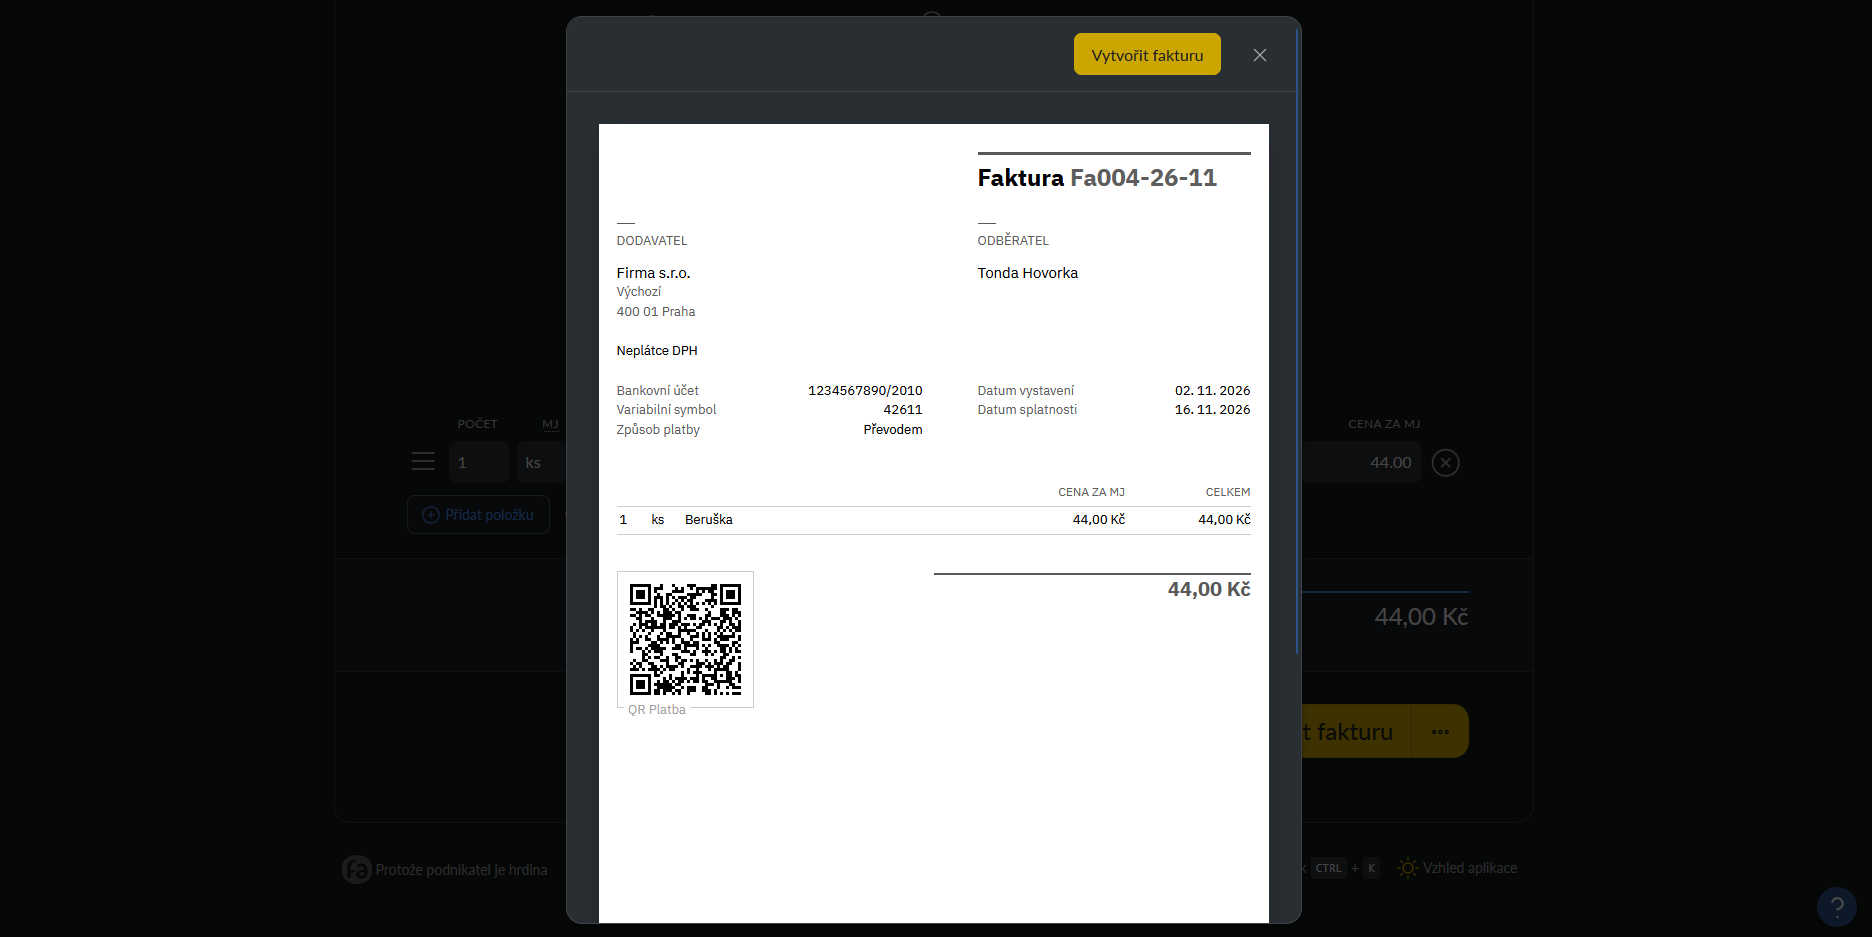
\includegraphics[width=0.85\linewidth]{obrazky/reserse/fakturoid_nahled_faktury.png}
\caption{Náhled faktury před jejím vystavením v~aplikaci Fakturoid (zdroj: vlastní snímek obrazovky ze zkušební verze, pořízeno 2.~11.~2026)}\label{obr:fakturoid-nahled}
\end{figure}

Řada prvků rozhraní je však nejasná. Cenové nabídky, šablony i~ceník jsou umístěny jako podzáložky v~sekci \emph{Faktury}. Šablony přitom neslouží ke změně vzhledu dokumentu, jak by název napovídal, ale k~uložení předvyplněné faktury pro opakované použití, a~pro nabídky nejsou k~dispozici vůbec. Vzhled dokumentu lze vybrat pouze ze šesti předdefinovaných variant. Po přechodu do ceníku se změní celá horní lišta a~uživatel ztratí přímý přístup k~fakturám a~nabídkám, aniž by mu rozhraní jasně ukázalo, ve které části aplikace se nachází. Stejné funkce jsou navíc dostupné z~více míst (z~tlačítka \enquote{+}, z~nabídky pod třemi tečkami a~z~hlavní navigace). Rušivě působí výrazná oznámení v~rámečku uprostřed obrazovky, která se zobrazují po každé akci, a~nápověda k~rychlým akcím, kterou se nepodařilo zavřít.

Přepsání čísla nabídky na vlastní tvar (například \texttt{NAB001-26}) formulář sice povolí, ale při uložení jej odmítne, protože neodpovídá formátu nastavenému pro číselnou řadu. Formát se nastavuje pomocí zástupných znaků, což je pro běžného uživatele zbytečně složité. Změnu jediného výchozího údaje, například splatnosti, nelze provést samostatně, ale jen přes celý formulář nastavení faktury. Nová ceníková položka se ve výchozím stavu zakládá jako skladová s~povinným množstvím, nákupní a~prodejní cenou, což servisní firma bez skladu nepotřebuje. Správa uživatelů a~oprávnění nebyla ve zkušební verzi dostupná.

Ve srovnání s~navrhovanou aplikací Fakturoid neobsahuje evidenci zakázek, zařízení ani provedené práce, materiál eviduje pouze formou skladu, neumožňuje vlastní šablony dokumentů a~místo kalendáře nabízí jen přehled a~statistiky. Cenové nabídky, sklad s~pohyby, upomínky a~více číselných řad jsou navíc dostupné až v~nejdražším tarifu \cite{fakturoid-srovnani}.

\subsection{Vhodnost pro malé firmy}

Fakturoid je velmi vhodný pro živnostníky a~malé firmy, které potřebují především rychle vystavovat faktury: nic se neinstaluje ani nespravuje, cena je nízká a~rozhraní přehledné. Servisní firma by však pokryla jen fakturační konec svého procesu a~evidenci zakázek by musela vést jinde. Data jsou uložena výhradně v~cloudu výrobce.

% Rešerše – iDoklad (vkládá se do kapitoly 01-reserse.tex)
\section{iDoklad}\label{sec:reserse-idoklad}

iDoklad je online fakturační a~evidenční služba ze skupiny, do které patří i~ekonomické systémy Money. Základní údaje shrnuje tabulka~\ref{tab:reserse-idoklad}.

\begin{table}[H]
\centering
\small
\begin{tabular}{>{\raggedright\arraybackslash}p{0.24\linewidth}>{\raggedright\arraybackslash}p{0.70\linewidth}}
\hline
\textbf{Kritérium} & \textbf{Zjištění} \\
\hline
Název & iDoklad \\
Společnost & Seyfor, a.s. (CZ; dříve Solitea) \cite{idoklad-web} \\
Typ aplikace & webová aplikace a~mobilní aplikace pro iOS a~Android \cite{idoklad-web,idoklad-vlastnosti} \\
Hostování & pouze cloud (SaaS provozovaný výrobcem); vlastní server ani lokální instalace nejsou možné \\
Licence & proprietární, předplatné \\
Cena & ceny bez DPH za měsíc při roční / čtvrtletní / měsíční platbě: Zdarma 0~Kč (1 uživatel, 5 kontaktů), Základní 187 / 220 / 240~Kč (2 uživatelé), Oblíbený 358 / 397 / 430~Kč (5 uživatelů), Prémiový 625 / 703 / 750~Kč (9 uživatelů) \cite{idoklad-cenik} \\
Zkušební verze & 60 dní v~tarifu Prémiový, bez platební karty; garance vrácení peněz do 30 dní \cite{idoklad-cenik,idoklad-vlastnosti} \\
\hline
\end{tabular}
\caption{Základní údaje o~řešení iDoklad}\label{tab:reserse-idoklad}
\end{table}

\subsection{Zkušenosti ze zkušební verze}

První dojem z~aplikace je velmi příjemný. Navigace je umístěna v~levém panelu s~ikonami, který lze zasunout a~získat tak více místa, což odpovídá návrhu navrhované aplikace. Výrazné zelené tlačítko \emph{Nový} umožňuje vytvořit libovolný doklad bez hledání v~záložkách. Tabulky faktur, nabídek i~ceníku vypadají jednotně, zobrazují jen potřebné sloupce a~další lze doplnit v~nastavení. Formulář cenové nabídky je totožný s~formulářem faktury, což usnadňuje orientaci. Sloupec se stavem dokladu přehledně ukazuje, v~jaké fázi se dokument nachází.

Formulář faktury zobrazuje poměrně mnoho údajů najednou, všechny však mají svůj smysl. Chybějící údaje jsou na rozdíl od Fakturoidu zobrazeny pouze jako varování ve spodní části formuláře a~doklad lze tlačítkem \emph{Přesto uložit} uložit i~s~nimi (obrázek~\ref{obr:idoklad-faktura}). Pořadové číslo dokladu lze změnit, formát číselné řady se ale nastavuje zástupnými znaky podobně jako ve Fakturoidu, i~když nápověda jejich význam vysvětluje. Tisk zobrazí náhled dokumentu, vzhled je však možné volit jen z~předdefinovaných variant a~funkce \emph{Šablony} slouží, stejně jako ve Fakturoidu, pouze k~předvyplnění opakovaných dokladů. Ceníkové položky stačí zadat jen názvem, ostatní údaje nejsou povinné. Velmi zdařilá jsou drobná vyskakovací oznámení, která jsou výrazná, ale nepřekážejí a~rychle zmizí, a~panel upozornění, který by v~navrhované aplikaci mohl sloužit pro upomínky blížících se termínů nebo historii posledních změn.

\begin{figure}[H]
\centering
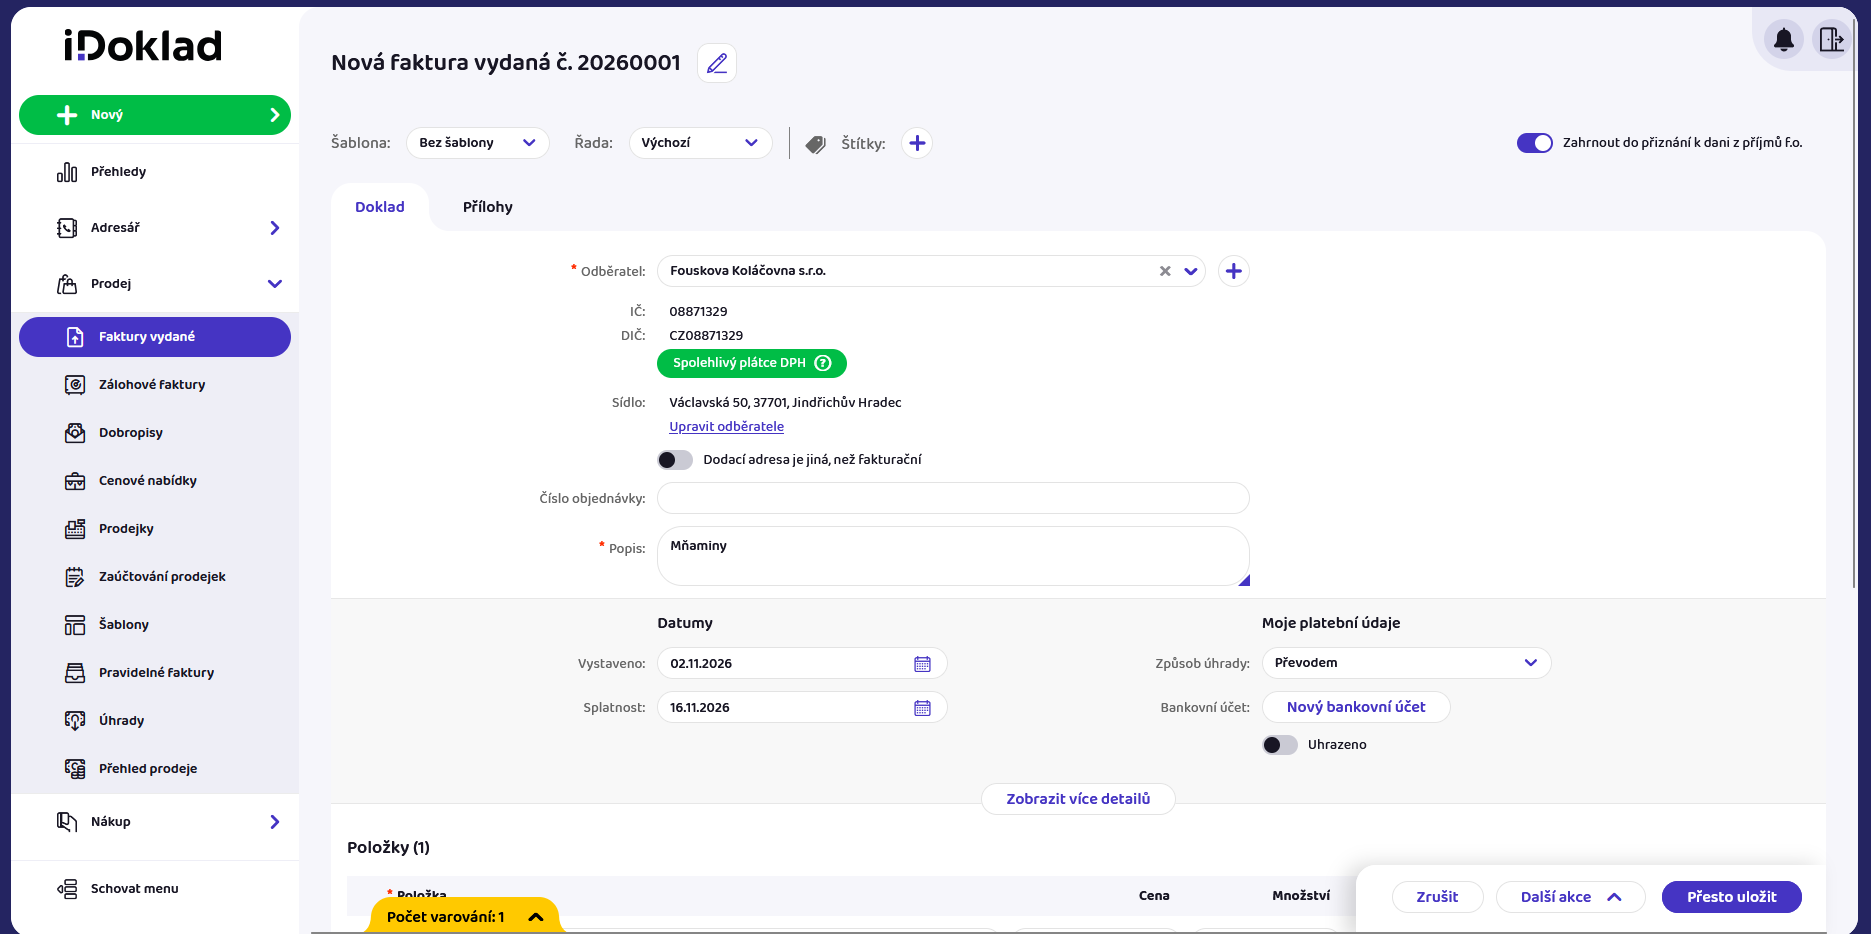
\includegraphics[width=\linewidth]{obrazky/reserse/iDoklad_tvorba_faktury.png}
\caption{Formulář nové faktury v~aplikaci iDoklad s~varováním o~chybějících údajích a~tlačítkem \emph{Přesto uložit} (zdroj: vlastní snímek obrazovky ze zkušební verze, pořízeno 2.~11.~2026)}\label{obr:idoklad-faktura}
\end{figure}

Nevýhodou je velké množství ikon s~akcemi přímo v~seznamu dokladů, z~nichž řada není pro běžnou práci potřeba a~stačila by v~detailu dokladu. Filtrování podle stavu (\emph{Všechny}, \emph{Uhrazené} atd.) je řešeno samostatnými položkami v~menu, přitom by stačil štítek se stavem u~každého dokladu a~filtr v~tabulce. Některé stránky nemají tlačítko \enquote{Zpět} a~ikona v~pravém horním rohu, která by jej mohla nahrazovat, uživatele odhlásí. Právě proto se navrhovaná aplikace drží doporučené zásady konzistence: tlačítka se stejným účelem mají na všech obrazovkách stejné umístění i~vzhled (oddíl~\ref{sec:ui-soulad}). Stejné nastavení seznamu je dostupné ze dvou různých tlačítek a~ve spodní části obrazovky se opakovaně zobrazuje propagace aplikace. Sekce Nákup (přijaté faktury, účtenky, Inbox) a~řada dokladů v~sekci Prodej (zálohové faktury, dobropisy, prodejky, pravidelné faktury) přesahují potřeby malé servisní firmy. Zajímavou inspirací pro možné rozšíření je naopak sekce Finance s~pokladnou pro evidenci hotovostních plateb.

Stejně jako Fakturoid je iDoklad primárně fakturační aplikace a~chybí v~něm evidence zakázek, zařízení, provedené práce a~kalendář.

\subsection{Vhodnost pro malé firmy}

iDoklad je vhodný pro živnostníky a~malé obchodní firmy, zejména pokud spolupracují s~externí účetní, která používá systémy Money nebo Pohoda \cite{idoklad-ucetni}. Jednotné a~přehledné rozhraní a~dlouhá zkušební doba usnadňují začátek. Pro servisní firmu ale pokryje opět jen fakturaci, data jsou uložena výhradně v~cloudu výrobce a~vyšší tarify jsou dražší než u~Fakturoidu.

% Rešerše – ABRA (vkládá se do kapitoly 01-reserse.tex)
\section{ABRA}\label{sec:reserse-abra}

Společnost ABRA Software nabízí dva produkty: ekonomický systém \emph{ABRA Flexi} (dříve FlexiBee) pro malé a~střední firmy a~ERP \emph{ABRA Aiva} pro střední a~velké firmy. Pro srovnání byla zvolena ABRA Flexi, která jako jediná nabízí zkušební verzi a~cílí na menší firmy. Základní údaje shrnuje tabulka~\ref{tab:reserse-abra}.

\begin{table}[H]
\centering
\small
\begin{tabular}{>{\raggedright\arraybackslash}p{0.24\linewidth}>{\raggedright\arraybackslash}p{0.70\linewidth}}
\hline
\textbf{Kritérium} & \textbf{Zjištění} \\
\hline
Název & ABRA Flexi (pro větší firmy ABRA Aiva) \\
Společnost & ABRA Software s.r.o., Praha (CZ); přibližně 35 let na trhu, přes 7~300 zákaznických firem \cite{abra-web} \\
Typ aplikace & webová aplikace a~desktopový klient pro Windows, Linux i~macOS \cite{abra-flexi-cenik} \\
Hostování & primárně cloud výrobce (Amazon Web Services); vlastní server je možný jen s~placenou rozšířenou podporou \cite{abra-flexi-cenik} \\
Licence & proprietární, předplatné bez vstupního poplatku \cite{abra-web} \\
Cena & za pojmenovaného uživatele a~měsíc při měsíční / roční platbě: Basic 425 / 390~Kč, Business 1~055 / 967~Kč, Premium 1~375 / 1~260~Kč; uživatelé pouze pro čtení zdarma; ABRA Aiva jen na poptávku, nasazení v~řádu stovek tisíc až milionů korun \cite{abra-flexi-cenik,abra-aiva-cena} \\
Zkušební verze & 30 dní všech tarifů, bez platební karty \cite{abra-flexi-cenik} \\
\hline
\end{tabular}
\caption{Základní údaje o~řešení ABRA}\label{tab:reserse-abra}
\end{table}

\subsection{Zkušenosti ze zkušební verze}

První dojem z~aplikace je velmi pozitivní, systém působí všestranně. Hned při založení účtu lze nastavit vzhled aplikace a~velikost písma, takže rozhraní je přehledné a~čitelné. Pro vyzkoušení si lze nechat vygenerovat ukázková data. Úvodní nástěnka zobrazuje souhrny a~grafy, které jsou příjemné, ale pro potřeby servisní firmy nejsou podstatné. Navigace je stejně jako u~iDokladu v~levém panelu, který lze zúžit jen na ikony. Modré tlačítko \emph{Nový} v~pravém horním rohu je dobře viditelné a~odlišené od ostatních prvků, formuláře mají v~pravém dolním rohu jednotná tlačítka \emph{Zavřít} a~\emph{Uložit a~zavřít}. Sekce \emph{Všechny agendy} umožňuje připnout si do menu jen potřebné části systému, což odpovídá myšlence navrhované aplikace, tedy funkčnímu jádru s~volitelnými rozšířeními.

Tabulky (adresář firem, vydané faktury) jsou jednotné a~přehledné, ale ve výchozím stavu zobrazují velké množství sloupců. Lze si nastavit zobrazené sloupce i~uložit vlastní pohledy, což je dobrý nápad, avšak pro malou firmu zbytečně složitý; po každé změně filtru či řazení navíc aplikace nabízí uložení pohledu. Filtrování se otevírá v~postranním panelu, který zbytek obrazovky zašedne. Detail záznamu se otevře jen kliknutím na sloupec \emph{Interní číslo}, nikoli na celý řádek, což není na první pohled patrné. Stav úhrady je zobrazen procentem zaplacené částky místo srozumitelného stavu (odesláno, zaplaceno). Inspirativní je naopak souhrn počtu dokladů a~jejich celkové částky ve spodní části tabulky. Formulář nové firmy obsahuje velké množství polí; pro potřeby servisní firmy by stačila základní část s~kontaktní osobou a~přílohami. Pozitivně lze hodnotit i~systém upozornění, který se zapíná v~nastavení a~nezakrývá obsah obrazovky. Globální vyhledávání v~horní části je naopak příliš obecné a~často vede do nastavení místo k~hledanému záznamu.

Zásadní rozdíl je v~pojetí zakázky (obrázek~\ref{obr:abra-zakazka}). Zakázka v~ABRA Flexi je chápána jako obchodní příležitost s~předpokládanými náklady a~ziskem, nikoli jako evidence přijatého zařízení a~průběhu opravy. Nabídky, objednávky a~zakázky jsou navíc dostupné až v~tarifu Business za 1~055~Kč za uživatele měsíčně. Tisk dokumentů nabízí výběr tiskové sestavy, možnost upravit vzhled dokumentu podle vlastní šablony se však v~uživatelském rozhraní nepodařilo najít, přestože nápověda popisuje konfigurovatelné reporty pro vybrané doklady \cite{abra-flexi-reporty}. Evidence zařízení, provedené práce a~kalendář v~systému chybí a~materiál je řešen pouze jako sklad.

\begin{figure}[H]
\centering
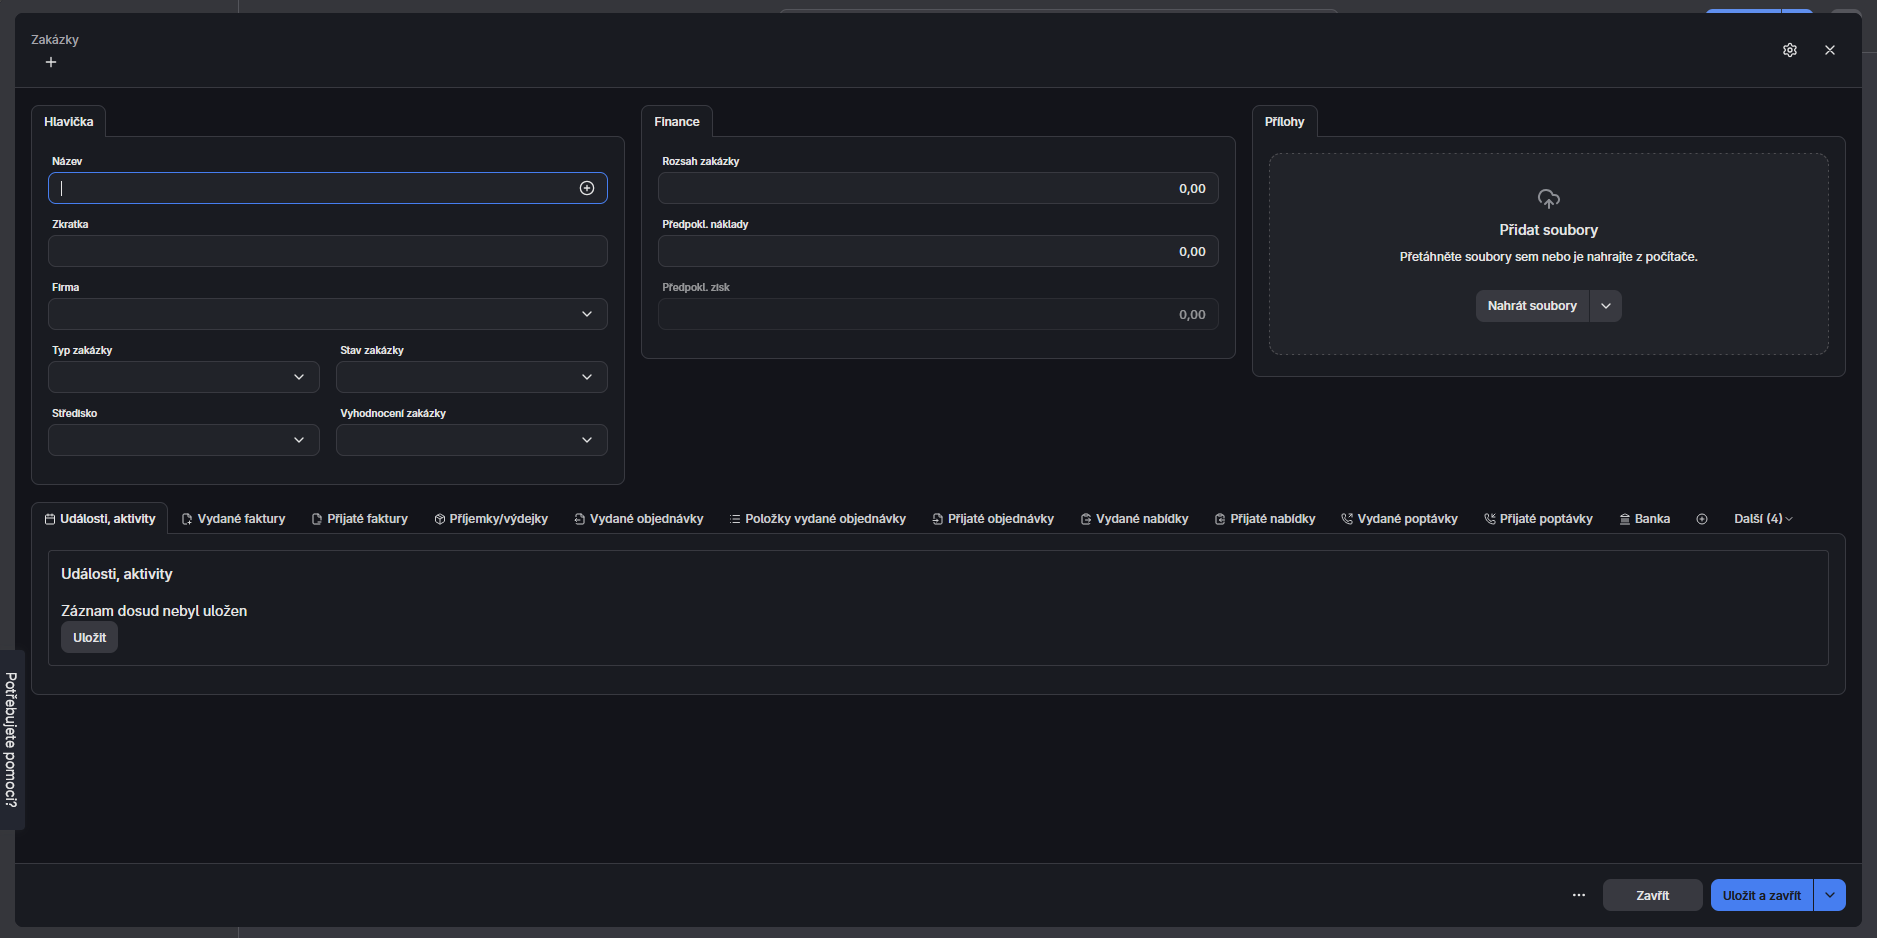
\includegraphics[width=\linewidth]{obrazky/reserse/abra_pridani_zakazky.png}
\caption{Formulář nové zakázky v~ABRA Flexi: zakázka je pojata jako obchodní případ s~rozsahem, náklady a~ziskem (zdroj: vlastní snímek obrazovky ze zkušební verze, pořízeno 3.~11.~2026)}\label{obr:abra-zakazka}
\end{figure}

\subsection{Vhodnost pro malé firmy}

ABRA Flexi je vhodná pro malé firmy, které chtějí vést kompletní účetnictví a~daňovou evidenci samy. Pro malou servisní firmu však nemá přiměřený poměr ceny a~přínosu: tarif Basic obsahuje z~potřebných funkcí v~podstatě jen fakturaci, kterou levněji nabízejí fakturační nástroje, a~tarif Business, který se potřebám firmy blíží nejvíce, stojí přes 1~000~Kč za uživatele měsíčně, a~přesto neobsahuje servisní evidenci. Rozhraní je přehledné a~přizpůsobitelné, ale orientované na zkušené administrativní a~účetní pracovníky.

% Rešerše – ERPNext (vkládá se do kapitoly 01-reserse.tex)
\section{ERPNext}\label{sec:reserse-erpnext}

ERPNext je open-source podnikový systém postavený na frameworku Frappe v~jazyce Python. Základní údaje shrnuje tabulka~\ref{tab:reserse-erpnext}.

\begin{table}[H]
\centering
\small
\begin{tabular}{>{\raggedright\arraybackslash}p{0.24\linewidth}>{\raggedright\arraybackslash}p{0.70\linewidth}}
\hline
\textbf{Kritérium} & \textbf{Zjištění} \\
\hline
Název & ERPNext \\
Společnost & Frappe Technologies Pvt. Ltd. (Indie) a~komunita; první verze v~roce 2010 \cite{wiki-erpnext} \\
Typ aplikace & webová aplikace (Python, framework Frappe, databáze MariaDB) \cite{wiki-erpnext,erpnext-web} \\
Hostování & vlastní server zdarma, nebo cloud Frappe Cloud \cite{erpnext-cenik} \\
Licence & open-source, GNU GPL v3; žádné funkce nejsou zpoplatněny \cite{erpnext-github,erpnext-web} \\
Cena & software zdarma; Frappe Cloud se neplatí za uživatele, ale podle výkonu: sdílený hosting od 5~USD, vlastní server od 20~USD měsíčně \cite{erpnext-cenik} \\
Zkušební verze & 14 dní na Frappe Cloud \cite{erpnext-cenik} \\
\hline
\end{tabular}
\caption{Základní údaje o~řešení ERPNext}\label{tab:reserse-erpnext}
\end{table}

\subsection{Zkušenosti ze zkušební verze}

Průvodce prvním nastavením se zobrazil v~angličtině a~aplikace byla proto hodnocena v~anglickém prostředí. Projekt sice obsahuje komunitní český překlad rozhraní \cite{erpnext-github}, oficiální česká lokalizace (například podpora formátu ISDOC nebo českých daňových výkazů) však neexistuje \cite{frappe-forum-cz}.

Rozhraní působí minimalisticky a~přehledně: v~levé části je lišta s~ikonami modulů, jejichž název se zobrazí po najetí myší, a~vedle ní seznam podkategorií. Sekce \emph{Setup} nabízí velké množství možností, od správy uživatelů, organizace a~přístupových rolí po nastavení tiskových dokumentů, včetně úpravy hlavičky dokumentu v~jazyce HTML. Všechny volby jsou přehledné a~tlačítka pro uložení nebo přidání záznamu jasně viditelná, celkově však aplikace působí jako nástroj pro zkušeného administrátora, který si systém sám nastaví, nikoli pro běžného zaměstnance malé firmy. Bez zaškolení by úvodní nastavení zabralo několik hodin. Příjemně jednoduché je založení nového uživatele, kde stačí vyplnit e-mail a~jméno, s~možností zobrazit celý formulář. Panel upozornění je funkční (všechna upozornění nebo jen nadcházející události), ale zobrazuje se přes celou výšku stránky a~zakrývá obsah (obrázek~\ref{obr:erpnext-upozorneni}). Evidence zakázek je vedena prostřednictvím projektů, takže každá servisní zakázka by musela být založena jako samostatný projekt, což je pro servisní praxi zbytečná administrativní zátěž.

\begin{figure}[H]
\centering
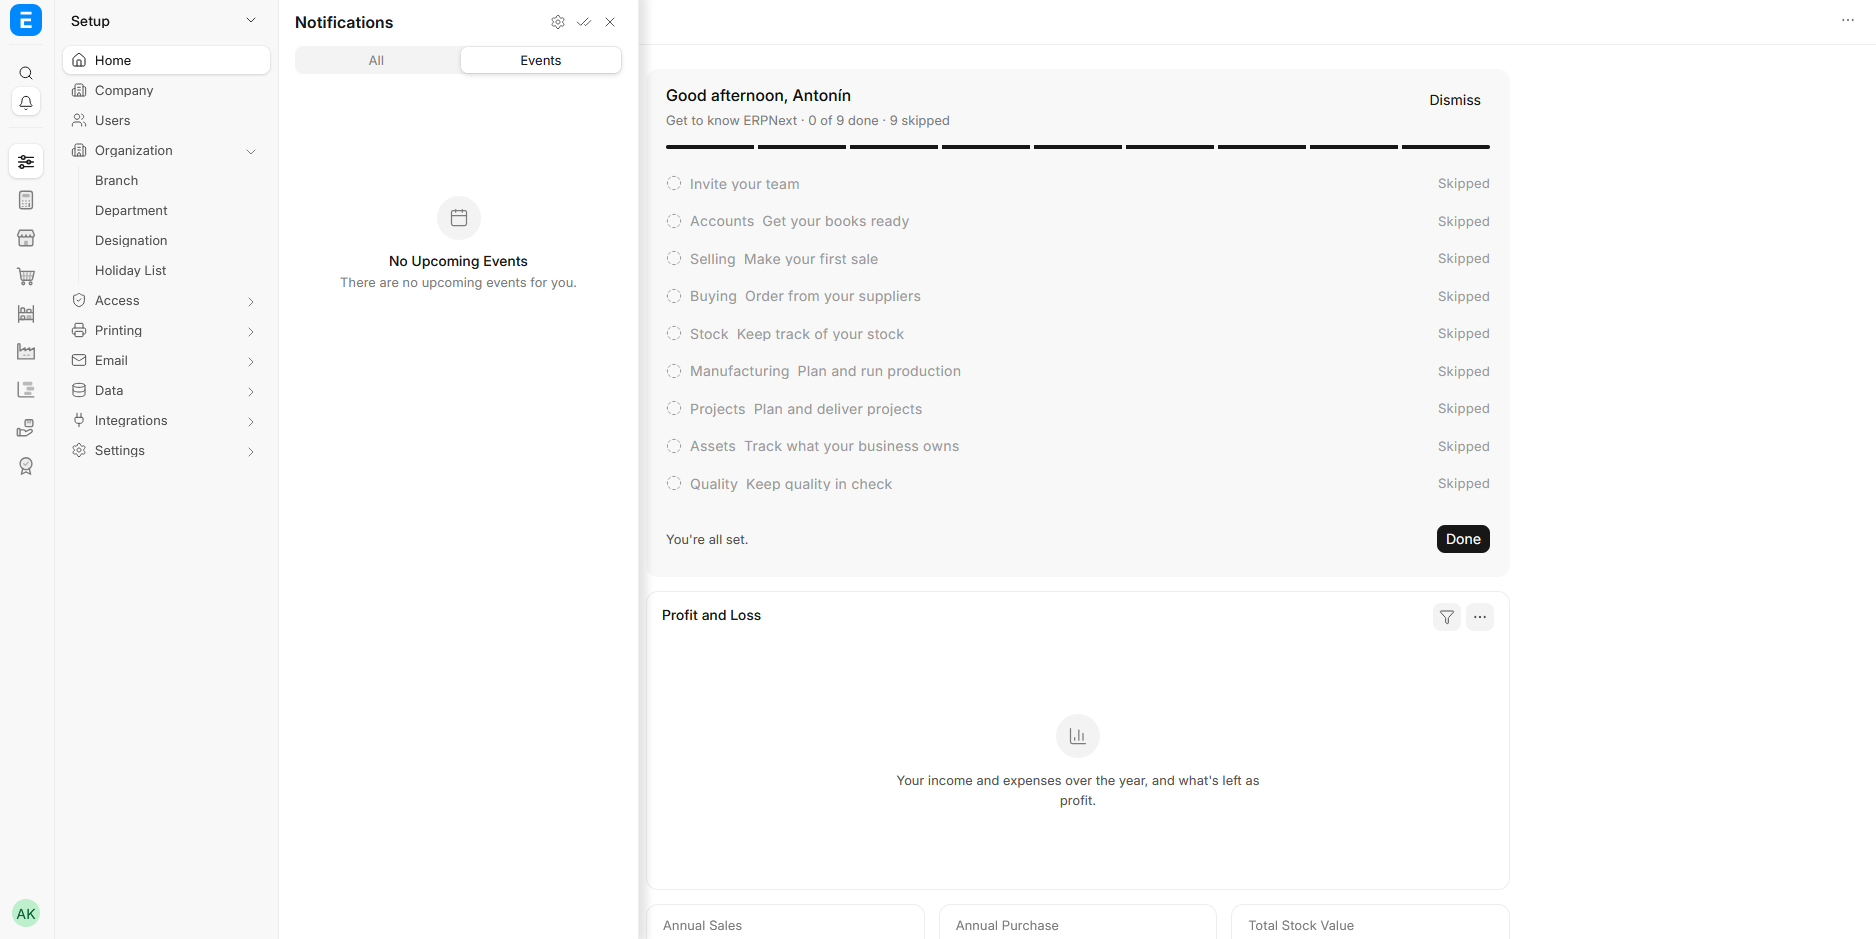
\includegraphics[width=\linewidth]{obrazky/reserse/erpnext_upozorneni.png}
\caption{Panel upozornění v~ERPNext zobrazený přes celou výšku stránky (zdroj: vlastní snímek obrazovky ze zkušební verze, pořízeno 3.~11.~2026)}\label{obr:erpnext-upozorneni}
\end{figure}

\subsection{Vhodnost pro malé firmy}

Cenově je ERPNext pro malou firmu velmi vhodný: software je zdarma a~cloudový provoz se neplatí za uživatele. Překážkou je však chybějící česká lokalizace, nedostatek implementačních partnerů v~České republice a~náročnost nastavení i~vlastního provozu, který vyžaduje znalost Linuxu, Pythonu a~databáze MariaDB. Pro malou servisní firmu bez technického zázemí je proto nasazení obtížné. Architekturou, tedy open-source webovou aplikací v~jazyce Python, je však ze všech srovnávaných řešení navrhované aplikaci nejblíže.

% Rešerše – Odoo (vkládá se do kapitoly 01-reserse.tex)
\section{Odoo}\label{sec:reserse-odoo}

Odoo je modulární podnikový systém složený z~desítek aplikací, ze kterých si firma vybírá jen ty, které potřebuje. Základní údaje shrnuje tabulka~\ref{tab:reserse-odoo}.

\begin{table}[H]
\centering
\small
\begin{tabular}{>{\raggedright\arraybackslash}p{0.24\linewidth}>{\raggedright\arraybackslash}p{0.70\linewidth}}
\hline
\textbf{Kritérium} & \textbf{Zjištění} \\
\hline
Název & Odoo (dříve TinyERP a~OpenERP) \\
Společnost & Odoo S.A., Belgie; zakladatel a~generální ředitel Fabien Pinckaers \cite{wiki-odoo,odoo-zdrazeni} \\
Typ aplikace & webová aplikace a~mobilní aplikace \\
Hostování & cloud výrobce (Odoo Online), platforma Odoo.sh i~vlastní server \cite{wiki-odoo,odoo-cenik} \\
Licence & dvě edice: Community jako open-source (LGPLv3), Enterprise jako proprietární předplatné \cite{wiki-odoo,odoo-github} \\
Cena & Community zdarma; v~cloudu je jedna aplikace zdarma s~neomezeným počtem uživatelů; tarif Standardní 11,90~€ (běžně 14,90~€) a~Nestandardní 22,90~€ (běžně 27,90~€) za uživatele a~měsíc; vlastní server, úpravy přes Odoo Studio a~API jen v~tarifu Nestandardní (obrázek~\ref{obr:odoo-cenik}) \cite{odoo-cenik}; implementace u~českých partnerů pro malou firmu přibližně 150 až 400 tisíc~Kč \cite{elfox-odoo} \\
Zkušební verze & 15 dní pro více aplikací, jedna aplikace je zdarma trvale \cite{odoo-cenik} \\
\hline
\end{tabular}
\caption{Základní údaje o~řešení Odoo}\label{tab:reserse-odoo}
\end{table}

\begin{figure}[H]
\centering
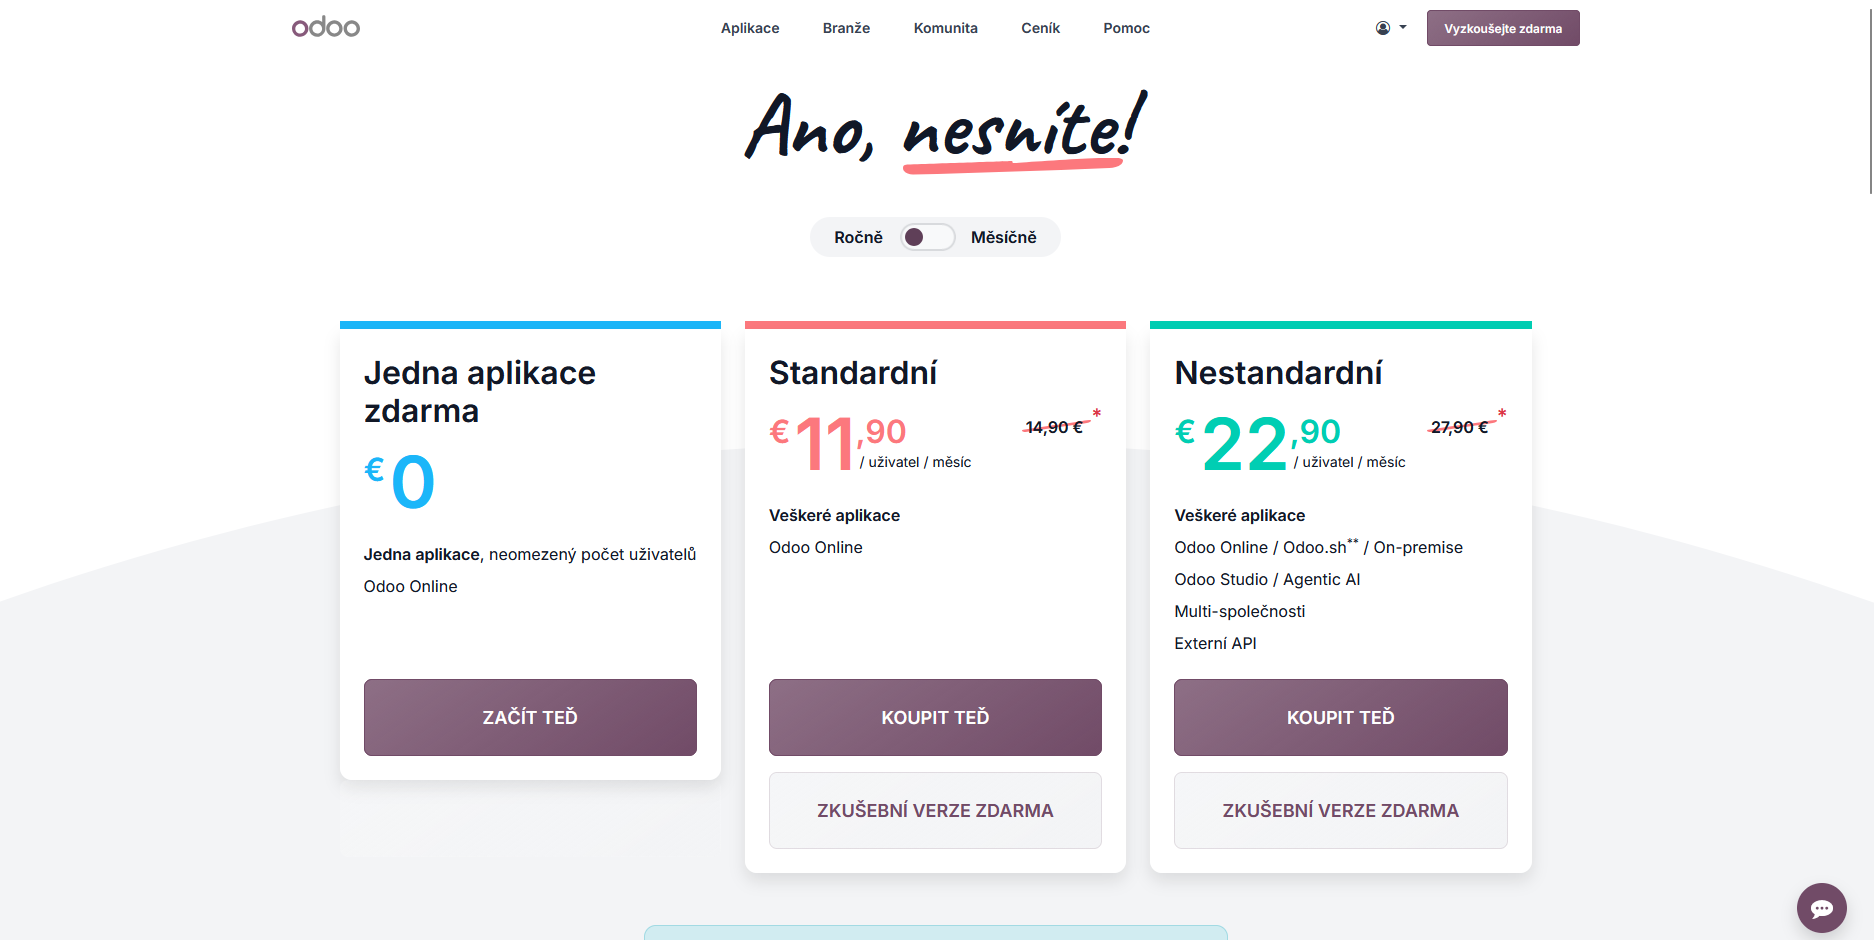
\includegraphics[width=0.9\linewidth]{obrazky/reserse/odoo_cenik_predplatne.png}
\caption{Ceník Odoo pro Českou republiku (zdroj: vlastní snímek obrazovky stránky \protect\url{https://www.odoo.com/cs_CZ/pricing}, pořízeno 3.~11.~2026)}\label{obr:odoo-cenik}
\end{figure}

\subsection{Zkušenosti ze zkušební verze}

Ve zkušební verzi byly vybrány aplikace CRM, Pokladní systém, Fakturace, Dokumenty, Opravy a~Zaměstnanci. Odoo bylo vyzkoušeno jako poslední, protože od něj byl na základě předchozí rešerše očekáván největší přínos. Úvodní obrazovka působí přívětivě: barevné ikony jednotlivých aplikací na tmavém pozadí s~názvy, název firmy a~přihlášený uživatel v~pravém horním rohu. Důležitá tlačítka, například \emph{Nové}, jsou barevně odlišená a~horní lišta ukazuje, ve které části aplikace se uživatel nachází. Tabulky jsou přehledné a~lze je přepnout do zobrazení kanban, seznam, graf nebo kalendář; kanbanové zobrazení kontaktů s~kartami obsahujícími jen základní údaje je velmi přehledné a~je inspirací pro navrhovanou aplikaci. Formulář nového kontaktu má vlevo vstupní pole a~vpravo souhrnný přehled, podobně jako v~navrhované aplikaci, záznam se však ukládá automaticky bez tlačítka \emph{Uložit}, takže uživatel nemá jistotu, zda byl uložen. Stránka Dokumenty se stromem složek je přehledná a~usnadňuje hledání v~uložených souborech. Příjemná je také sekce Aplikace, kde lze aplikace kdykoliv přidat nebo odebrat.

Aplikace Opravy umožňuje založit opravu výrobku i~nový výrobek přímo z~formuláře (obrázek~\ref{obr:odoo-opravy}). Stavy opravy jsou ale jen tři (\emph{Nové}, \emph{Potvrzený} a~\emph{Done}), částečně nepřeložené. Po dokončení opravy lze tlačítkem \emph{Invoice} vytvořit fakturu. Detail faktury nabízí akce Odeslat, Tisk, Zaplatit a~Náhled; tisk však bez náhledu rovnou stáhne soubor PDF a~po jednorázovém výběru vzhledu dokumentu (\emph{Setup your invoice layout}) se možnost jej znovu změnit nepodařilo najít. Nastavit formát číslování dokumentů nelze.

\begin{figure}[H]
\centering
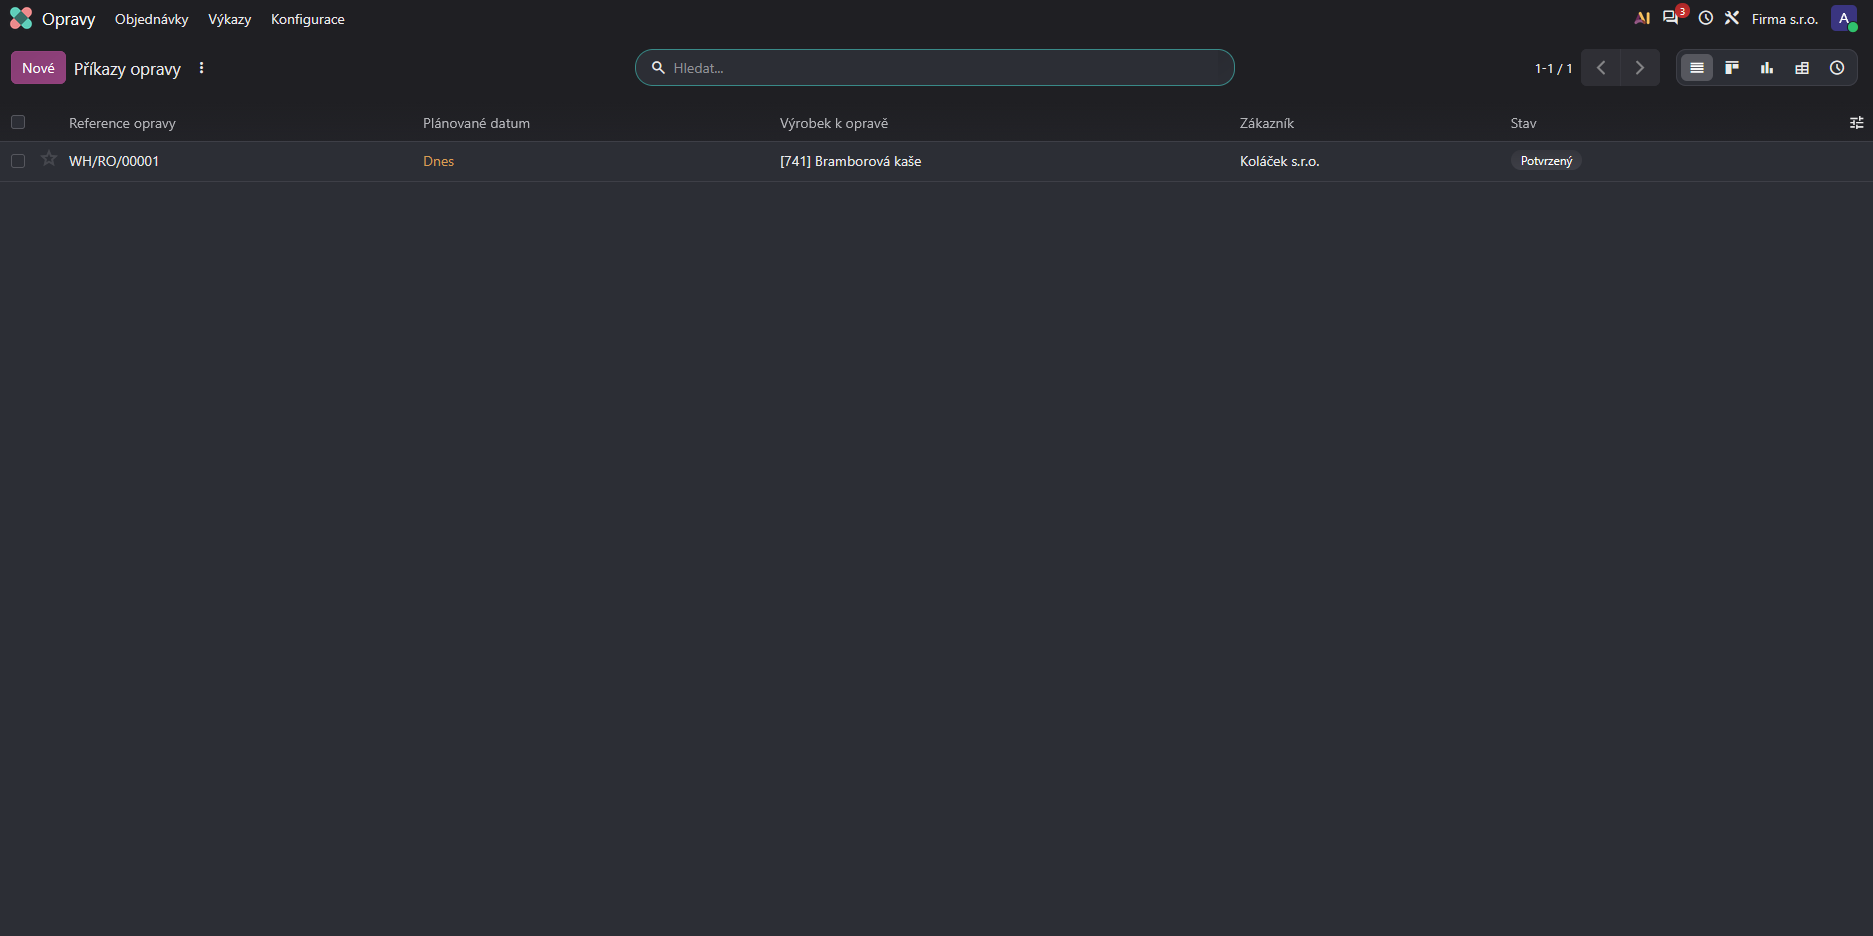
\includegraphics[width=\linewidth]{obrazky/reserse/odoo_strana_opravy.png}
\caption{Seznam oprav v~aplikaci Odoo s~přepínáním zobrazení vpravo nahoře (zdroj: vlastní snímek obrazovky ze zkušební verze, pořízeno 3.~11.~2026)}\label{obr:odoo-opravy}
\end{figure}

Celkový dojem je přesto zklamáním. Navigace je nelogická: odkazy jako \emph{Objednávky} v~aplikaci Opravy vedou na tutéž stránku, \emph{Výkazy} zobrazí jen graf, nabídky jsou skryté pod položkou \emph{Objednávky} a~položky \emph{Zákazníci} a~\emph{Dodavatelé} v~aplikaci Fakturace pouze otevírají další nabídku, takže k~vytvoření faktury vede několik nepřímých kroků. Rozhraní je přeloženo jen částečně, anglické texty se objevují v~tlačítkách i~vstupních polích. Popisky ikon pro přepínání zobrazení se zobrazují pod kurzorem, který je zakrývá. Pravou část každého formuláře zabírá panel s~chatem, historií změn a~aktivitami určený pro spolupráci více zaměstnanců; zabírá téměř polovinu obrazovky, nelze změnit jeho velikost a~pro firmu s~jedním administrativním pracovníkem je zbytečný. Tlačítka \emph{Zrušit} a~\emph{Uložit} v~nastavení bez provedených změn nedělají nic viditelného, chybí tlačítko \enquote{Zpět} (nahrazuje jej jen malý křížek) a~po výběru sekce se nejprve zobrazí přehled s~grafy. Ve srovnání s~navrhovanou aplikací chybí evidence zařízení (aplikace Opravy tento požadavek nesplňuje), servisních zakázek a~provedené práce, materiál je dostupný jen jako součást skladu a~nelze použít vlastní šablony dokumentů.

\subsection{Vhodnost pro malé firmy}

Pokud by firma řešila pouze fakturaci, je Odoo díky trvale bezplatné jedné aplikaci výhodnější než placené fakturační služby. Pro pokrytí potřeb servisní firmy by však musela používat více aplikací v~placeném tarifu za přibližně 12~€ za uživatele měsíčně, a~ani tak by servisní evidence neodpovídala jejím požadavkům. Edice Community je zdarma, ale její provoz na vlastním serveru vyžaduje technické znalosti a~implementace u~partnera se pohybuje ve stovkách tisíc korun. Odoo je tak funkčně silné, ale pro malou servisní firmu provozně i~ekonomicky náročné a~vhodné spíše pro firmy, které počítají s~růstem.

% Rešerše – HELIOS (vkládá se do kapitoly 01-reserse.tex)
\section{HELIOS}\label{sec:reserse-helios}

Informační systémy HELIOS tvoří produktovou řadu od HELIOS Red pro živnostníky přes HELIOS Easy pro malé firmy a~HELIOS iNuvio pro malé a~střední firmy po HELIOS Nephrite pro velké firmy \cite{autoerp-srovnani}. Pro srovnání byl zvolen HELIOS iNuvio, nástupce rozšířeného systému HELIOS Orange. Základní údaje shrnuje tabulka~\ref{tab:reserse-helios}.

\begin{table}[H]
\centering
\small
\begin{tabular}{>{\raggedright\arraybackslash}p{0.24\linewidth}>{\raggedright\arraybackslash}p{0.70\linewidth}}
\hline
\textbf{Kritérium} & \textbf{Zjištění} \\
\hline
Název & HELIOS iNuvio (řada HELIOS Red, Easy, iNuvio, Nephrite) \\
Společnost & Asseco Solutions, a.s., Praha (CZ); přes 15~000 zákazníků \cite{helios-fenix-pl} \\
Typ aplikace & desktopová aplikace pro Windows v~architektuře klient--server nad databází Microsoft SQL Server \cite{helios-pozadavky} \\
Hostování & vlastní server nebo jediný počítač, vzdálený přístup přes vzdálenou plochu; cloud jako samostatná služba výrobce nebo u~partnerů \cite{helios-pozadavky,helios-inuvio,appon-inuvio} \\
Licence & proprietární \\
Cena & nezveřejněna, stanovuje se individuálně po analýze potřeb firmy; implementace trvá měsíce \cite{helios-inuvio,autoerp-srovnani} \\
Zkušební verze & není, pouze předváděcí demo na vyžádání \cite{helios-inuvio} \\
\hline
\end{tabular}
\caption{Základní údaje o~řešení HELIOS}\label{tab:reserse-helios}
\end{table}

\subsection{Zhodnocení}

HELIOS nenabízí zkušební verzi ani interaktivní ukázku, a~uživatelské rozhraní proto nebylo možné vlastnoručně vyzkoušet. Potenciální zákazník nemá možnost ověřit, zda systém odpovídá jeho potřebám, aniž by kontaktoval obchodní oddělení výrobce. Podle výrobce obsahuje HELIOS iNuvio ekonomiku, sklady, obchod s~CRM, lidské zdroje, výrobu, dopravu a~modul řízení projektů a~servisu \cite{helios-inuvio}, k~dispozici je otevřené API a~napojení na registr ARES \cite{ucetnictvi-inuvio}. Podrobný popis servisních funkcí však výrobce veřejně nezveřejňuje.

\subsection{Vhodnost pro malé firmy}

Pro malou firmu je HELIOS iNuvio málo vhodný. Vyžaduje vlastní server s~operačním systémem Windows nebo placený hosting, licence a~implementaci na míru, a~neveřejná cena spolu s~chybějící zkušební verzí brání rychlému rozhodnutí. Systém je určen středním a~větším firmám se složitými procesy, jako je výroba, rozsáhlé sklady nebo mzdy.


\section{Souhrnné srovnání}\label{sec:reserse-srovnani}

Tabulka~\ref{tab:reserse-souhrn} shrnuje základní charakteristiky všech srovnávaných řešení. Pro úplnost je v~ní uvedena i~navrhovaná aplikace BusinessManager.

\begin{table}[htbp]
\centering
\footnotesize
\setlength{\tabcolsep}{3pt}
\resizebox{\textwidth}{!}{%
\begin{tabular}{>{\raggedright\arraybackslash}p{2.0cm}>{\raggedright\arraybackslash}p{2.4cm}>{\raggedright\arraybackslash}p{1.5cm}>{\raggedright\arraybackslash}p{2.3cm}>{\raggedright\arraybackslash}p{1.9cm}>{\raggedright\arraybackslash}p{2.7cm}>{\raggedright\arraybackslash}p{1.8cm}}
\hline
\textbf{Řešení} & \textbf{Společnost} & \textbf{Typ} & \textbf{Hostování} & \textbf{Licence} & \textbf{Cena (měsíčně)} & \textbf{Vhodnost pro malou firmu} \\
\hline
Fakturoid & Fakturoid s.r.o. (CZ) & web, mobil & cloud & proprietární & 0--519 Kč s DPH & vysoká (jen fakturace) \\
iDoklad & Seyfor, a.s. (CZ) & web, mobil & cloud & proprietární & 0--750 Kč bez DPH & vysoká (jen fakturace) \\
ABRA Flexi & ABRA Software s.r.o. (CZ) & web, desktop & cloud (vlastní server s příplatkem) & proprietární & 390--1 375 Kč za uživatele & střední \\
ERPNext & Frappe Technologies (IN) & web & cloud i vlastní server & GPLv3 & zdarma;\newline cloud od 5~USD & střední (bez české lokalizace) \\
Odoo & Odoo S.A. (BE) & web, mobil & cloud i vlastní server & LGPLv3 / proprietární & jedna aplikace zdarma; 11,90--22,90 € za uživatele & střední \\
HELIOS iNuvio & Asseco Solutions, a.s. (CZ) & desktop (Windows) & vlastní server, cloud u partnerů & proprietární & na poptávku & nízká \\
\hline
Business\-Manager & vlastní řešení & web & vlastní server / lokální PC & open-source & zdarma & cílové řešení \\
\hline
\end{tabular}}
\caption{Souhrnné srovnání základních charakteristik řešení}\label{tab:reserse-souhrn}
\end{table}

Ze srovnání vyplývá, že řešení se dělí do dvou skupin. Fakturační nástroje Fakturoid a~iDoklad jsou levné, přehledné a~mají vyřešenou českou legislativu, nepokrývají však servisní část procesu: evidenci zařízení, zakázek, provedené práce ani kalendář. Podnikové systémy ABRA, ERPNext, Odoo a~HELIOS některé z~těchto oblastí obsahují, ale za cenu složitého rozhraní, nutnosti delšího zaškolení a~u~proprietárních řešení i~vyšších nákladů. Pojem zakázky navíc tyto systémy chápou jinak než servisní firma: ABRA jako obchodní příležitost, ERPNext jako projekt a~Odoo jako opravu výrobku s~velmi jednoduchými stavy. Žádné ze srovnávaných řešení tak nespojuje evidenci servisních zakázek a~zařízení, tvorbu dokumentů podle vlastních šablon, podporu formátu ISDOC, jednoduché rozhraní a~bezplatný provoz na vlastním počítači či serveru. Tato mezera je hlavním důvodem pro vývoj vlastní aplikace.

\section{Inspirace pro návrh aplikace}\label{sec:reserse-inspirace}

Rešerše přinesla řadu podnětů, které byly při návrhu aplikace využity, nebo jsou zaznamenány jako možná rozšíření:
\begin{itemize}
\item \textbf{Náhled dokumentu před jeho vytvořením} (Fakturoid, obrázek~\ref{obr:fakturoid-nahled}). Na rozdíl od Fakturoidu však aplikace náhled neblokuje kvůli nevyplněným údajům, pouze na ně upozorní.
\item \textbf{Upozornění místo blokování} (iDoklad, obrázek~\ref{obr:idoklad-faktura}): chybějící údaje jsou zobrazeny jako varování a~dokument lze přesto uložit. Podobně má aplikace upozornit na nevyplněné údaje o~firmě po první instalaci.
\item \textbf{Soukromá poznámka} k~dokladu (Fakturoid), oddělená od textu určeného zákazníkovi, například pro poznámky o~potřebném materiálu.
\item \textbf{Upozornění a~upomínky} (iDoklad, ABRA): přehled událostí, které je třeba vyřešit, například blížící se splatnost faktur nebo naposledy vytvořené dokumenty, aby další pracovník věděl, kde předchozí den skončila práce. V~aplikaci mohou vycházet z~části Kalendář.
\item \textbf{Souhrn počtu a~celkové částky dokladů} pod tabulkou (ABRA), zobrazovaný jen uživatelům s~oprávněním vidět finanční údaje; využití popisuje oddíl~\ref{sec:ui-inspirace}.
\item \textbf{Kanbanové zobrazení} zákazníků, zařízení či zakázek jako alternativa k~tabulce (Odoo); využití popisuje oddíl~\ref{sec:ui-inspirace}.
\item \textbf{Číslování dokumentů podle vzoru}: formát čísla se zadá ukázkou, například \texttt{NAB001-26}, místo složitého zápisu se zástupnými znaky, jaký používají Fakturoid a~iDoklad.
\item \textbf{Pokladna} pro evidenci hotovostních plateb (iDoklad) jako možný rozšiřující modul.
\end{itemize}
Naopak jako odstrašující příklady posloužily výrazná vyskakovací upozornění uprostřed obrazovky, zdvojené ovládací prvky se stejnou funkcí, chybějící tlačítko \enquote{Zpět} a~nejednotný jazyk rozhraní.

% ============================================================
% Teoretická část, bod 3: Zásady návrhu přehledného a efektivního
% uživatelského rozhraní
% Jen doporučení z literatury. Porovnání s rozhraním aplikace je
% v praktické části, oddíl sec:ui-soulad (kapitoly/navrh/ui-soulad.tex).
% ============================================================
\chapter{Zásady návrhu přehledného a~efektivního uživatelského rozhraní}\label{kap:uzivatelske-rozhrani}

\section{Význam uživatelského rozhraní v~podnikových aplikacích}

Uživatelské rozhraní představuje klíčový prvek každé softwarové aplikace, který významně ovlivňuje její použitelnost a~efektivitu v~praxi. V~případě podnikových aplikací, které jsou používány každodenně, má kvalita návrhu uživatelského rozhraní přímý dopad na rychlost práce, chybovost při zadávání údajů a~celkovou spokojenost uživatelů.

Špatně navržené rozhraní může vést k~neefektivní práci, zvýšené chybovosti a~odmítání aplikace ze strany uživatelů, zatímco přehledné a~srozumitelné rozhraní podporuje plynulý průběh pracovních procesů. Jordan et~al.\ řadí jednoduché ovládání mezi hlavní faktory úspěšného zavedení systému pro správu dokumentů \cite[s.~48]{Jordan2022}. Z~tohoto důvodu není návrh uživatelského rozhraní náhodný, ale vychází z~ověřených principů použitelnosti a~návrhu interakce, které shrnují následující oddíly.

\section{Uživatelský kontext a~cílová skupina}

Navrhovaná aplikace je určena především pro zaměstnance malé servisní firmy, kteří zajišťují administrativní zpracování zakázek, fakturaci a~související dokumentaci. Typickými uživateli jsou administrativní pracovníci, kteří pracují s~aplikací pravidelně v~rámci své každodenní pracovní činnosti.

Jedná se o~uživatele bez specializovaných IT znalostí, proto je nutné klást důraz na intuitivní ovládání, jasnou strukturu obrazovek a~srozumitelné popisy jednotlivých funkcí. Uživatelské rozhraní by mělo být navrženo tak, aby bylo snadno pochopitelné i~pro uživatele bez technického zázemí a~nevyžadovalo rozsáhlé školení. Shneiderman tento požadavek formuluje jako \emph{univerzální použitelnost}: rozhraní má počítat s~rozdílnými skupinami uživatelů, od začátečníků po zkušené \cite{Shneiderman-pravidla}.

\section{Obecné heuristiky použitelnosti}\label{sec:ui-heuristiky}

Nejrozšířenějším souborem zásad pro návrh rozhraní je deset heuristik použitelnosti, které sestavil Jakob Nielsen. Jde o~obecná pravidla, ne o~konkrétní návod, a~používají se i~pro hodnocení hotových rozhraní \cite{Nielsen-heuristiky}:
\begin{enumerate}
\item \textbf{Viditelnost stavu systému.} Uživatel má vždy vědět, co se děje, a~dostat včas zpětnou vazbu.
\item \textbf{Shoda systému s~reálným světem.} Rozhraní používá slova a~pojmy, které uživatel zná, a~informace řadí v~přirozeném pořadí.
\item \textbf{Kontrola a~svoboda uživatele.} Uživatel potřebuje jasně označený \enquote{nouzový východ}, kterým nechtěnou akci opustí nebo vrátí.
\item \textbf{Konzistence a~standardy.} Stejná slova a~akce mají znamenat totéž v~celé aplikaci.
\item \textbf{Prevence chyb.} Lepší než dobré chybové hlášení je návrh, který chybě předejde.
\item \textbf{Rozpoznání místo vybavování.} Prvky, akce a~volby mají být vidět, aby si je uživatel nemusel pamatovat.
\item \textbf{Flexibilita a~efektivita.} Zkušený uživatel má mít k~dispozici zkratky, které začátečníkovi nepřekáží.
\item \textbf{Estetický a~minimalistický design.} Rozhraní nemá obsahovat informace, které nejsou potřeba.
\item \textbf{Pomoc s~rozpoznáním a~opravou chyb.} Chybová hlášení mají být srozumitelná a~navrhnout řešení.
\item \textbf{Nápověda a~dokumentace.} Má být snadno dohledatelná a~zaměřená na úkol uživatele.
\end{enumerate}

Podobný soubor tvoří \emph{osm zlatých pravidel} Bena Shneidermana: usilovat o~konzistenci, usilovat o~univerzální použitelnost, poskytovat informativní zpětnou vazbu, navrhovat dialogy s~jasným zakončením, předcházet chybám, umožnit snadné vrácení akcí, ponechat uživateli kontrolu a~snižovat zátěž krátkodobé paměti \cite{Shneiderman-pravidla}. Wong ukazuje, že se obě sady pravidel z~velké části překrývají a~dohromady tvoří praktická \enquote{pravidla palce} pro návrh rozhraní \cite{Wong2025}.

Kaplan ukazuje, jak se heuristiky uplatní ve složitých podnikových aplikacích. Konzistenci dokládá příkladem, kdy je hlavní akce pro vytvoření nové položky ve všech pracovních prostorech na stejném místě, v~pravém horním rohu, a~vypadá stejně \cite{Kaplan2021}. K~minimalismu uvádí, že každá informace navíc soupeří s~informacemi důležitými a~ztěžuje jejich vyhledání. Zřídka používaná nastavení proto doporučuje skrýt, dokud nejsou potřeba \cite{Kaplan2021}.

\section{Zásady přehlednosti a~jednoduchosti}\label{sec:ui-prehlednost}

Jedním ze základních principů návrhu uživatelského rozhraní je přehlednost. Rozhraní by mělo být vizuálně jednoduché, bez nadbytečných prvků, které by uživatele zbytečně rozptylovaly. Minimalistický přístup umožňuje uživateli soustředit se na aktuálně vykonávaný úkol a~snižuje kognitivní zátěž. Sajedi et~al.\ doporučují zobrazovat jen informace potřebné pro aktuální úkol a~ostatní skrýt \cite[s.~2332]{Sajedi2011}. Rozhraní má být jednoduché a~složitější úkoly rozdělit do jednodušších kroků a~formulářů \cite[s.~2330]{Sajedi2011}.

Důležitým aspektem je také logické členění obrazovek a~jednoznačné rozdělení funkcí do samostatných částí aplikace. Uživatel by měl být schopen rychle se orientovat v~tom, kde se nachází a~jaké akce může v~daném kontextu provádět. Použití jednotného vizuálního stylu, konzistentního rozložení prvků a~jasné hierarchie informací přispívá k~celkové srozumitelnosti rozhraní \cite[s.~2328]{Sajedi2011}.

\emph{Postupné odhalování} (progressive disclosure) řeší rozpor mezi požadavkem na jednoduchost a~potřebou nabídnout všechny funkce. Na první obrazovce se zobrazí jen nejdůležitější volby a~méně používané funkce jsou až na další obrazovce, kam je uživatel otevře jen v~případě potřeby. Nielsen uvádí, že tím se zlepší učení, efektivita i~chybovost \cite{Nielsen-progressive}. Sajedi et~al.\ podobně doporučují funkce, ke kterým uživatel nemá oprávnění, podle situace zakázat nebo zcela skrýt \cite[s.~2331]{Sajedi2011}.

\section{Základní principy použitelnosti a~UX}\label{sec:ui-principy}

Návrh uživatelského rozhraní vychází ze základních principů použitelnosti a~uživatelské zkušenosti (UX). Mezi klíčové principy patří konzistence, srozumitelné ovládání a~předvídatelné chování aplikace.

Konzistence znamená jednotné používání ovládacích prvků, barev, ikon a~terminologie napříč celou aplikací \cite{Nielsen-heuristiky}. Díky tomu si uživatel rychle vytváří mentální model práce se systémem a~minimalizuje se riziko chyb. Sajedi et~al.\ dodávají, že barva má sloužit jen jako doplňkové vodítko a~informace nesmí záviset jen na ní \cite[s.~2329]{Sajedi2011}.

Dalším důležitým principem je minimalizace počtu kroků potřebných k~dosažení cíle. Uživatel by měl být schopen provádět běžné činnosti s~co nejmenším počtem interakcí, aniž by bylo nutné procházet složitými dialogy nebo nabídkami. Sajedi et~al.\ doporučují, aby systém sám doplňoval známé údaje a~pamatoval si předchozí volby uživatele \cite[s.~2331--2332]{Sajedi2011}. Často používané prvky mají být snadno dosažitelné. Podle Fittsova zákona se nejrychleji zasáhnou velké cíle a~cíle u~okrajů a~v~rozích obrazovky \cite[s.~2330]{Sajedi2011}.

Uživatel má mít nad aplikací kontrolu. Má mít možnost akci zrušit nebo vrátit a~systém ho má chránit před chybami, například potvrzením nevratné akce \cite[s.~2331--2332]{Sajedi2011}. U~složitějších formulářů má být k~dispozici stručná nápověda \cite[s.~2330]{Sajedi2011}.

\section{Navigace}\label{sec:ui-navigace}

Navigace má uživateli ukázat, kde se v~aplikaci nachází a~kam může pokračovat \cite[s.~2332--2333]{Sajedi2011}. Laubheimer doporučuje pro desktopové rozhraní svislou navigaci v~levé části obrazovky. Pojme více položek než vodorovná lišta, lze ji rozšiřovat bez přepracování celé struktury a~svislý seznam se rychleji prohlíží, protože uživatelé se nejčastěji dívají do levé poloviny obrazovky. Ikony bez textových popisků nedoporučuje, protože jsou nejednoznačné. Navigace sbalená jen na ikony je podle něj přijatelná u~aplikací používaných denně, kde se uživatelé položky naučí, ne však u~občas navštěvovaných webů \cite{Laubheimer2021}.

\section{Přístupnost}\label{sec:ui-pristupnost}

Pravidla přístupnosti webového obsahu WCAG~2.2 stanovují měřitelná kritéria, která pomáhají i~uživatelům se slabším zrakem nebo menší zručností \cite{WCAG22}. Pro aplikaci tohoto typu jsou podstatná zejména tato kritéria:
\begin{itemize}
\item \textbf{1.4.1 Použití barvy} -- barva nesmí být jediným prostředkem, který nese informaci;
\item \textbf{1.4.3 Kontrast} -- běžný text musí mít vůči pozadí kontrastní poměr alespoň 4,5\,:\,1;
\item \textbf{2.5.8 Velikost cíle} -- klikací prvky mají mít alespoň 24~$\times$~24 pixelů.
\end{itemize}

\section{Doporučení pro návrh uživatelského rozhraní}\label{sec:ui-doporuceni}

Na základě uvedených principů lze formulovat obecná doporučení pro návrh uživatelského rozhraní podnikové aplikace. Rozhraní by mělo obsahovat pouze funkce, které jsou skutečně využívány v~rámci pracovních procesů, a~vyhýbat se nadbytečným možnostem, které mohou působit matoucím dojmem. Funkce potřebné jen pro správu systému mají být oddělené a~dostupné jen těm, kdo je potřebují.

Důraz by měl být kladen na přehledné zobrazení klíčových informací, jednoznačné označení ovládacích prvků a~jasnou zpětnou vazbu o~provedených akcích. Hlavní akce má být na každé obrazovce na stejném místě, navigace svislá vlevo a~barvy doplněné textem. Takto navržené rozhraní podporuje efektivní práci uživatelů a~zvyšuje pravděpodobnost úspěšného nasazení aplikace v~reálném provozu. Jak tato doporučení naplňuje rozhraní aplikace, porovnává oddíl~\ref{sec:ui-soulad} v~praktické části.

% ============================================================
% Teoretická část, bod 4: Principy databázového návrhu
% Jen to, co doporučuje literatura (hlavně Silberschatz et al., 7. vyd.).
% Porovnání s návrhem databáze aplikace je v praktické části,
% oddíl sec:db-soulad (kapitoly/navrh/databaze-soulad.tex).
% ============================================================
\chapter{Principy databázového návrhu}\label{kap:principy-db}

Učebnice \emph{Database System Concepts} autorů Silberschatze, Kortha a~Sudarshana \cite{Silberschatz2020} patří ke standardním vysokoškolským učebnicím databázových systémů a~popisuje celý postup návrhu: od konceptuálního modelu přes převod na relační schéma až po normalizaci a~integritní omezení. Tato kapitola shrnuje principy z~této knihy, o~které se opírá návrh databáze. Jak se jednotlivé principy uplatnily v~databázi aplikace a~kde se od nich návrh záměrně odchyluje, popisuje oddíl~\ref{sec:db-soulad} v~praktické části.

\section{Relační model a~klíče}\label{sec:principy-klice}

Relační databáze ukládá data v~relacích (tabulkách), jejichž řádky musí být navzájem rozlišitelné podle hodnot atributů. Množina atributů, která jednoznačně určuje řádek, se nazývá \emph{nadklíč}; nadklíč, z~něhož nelze žádný atribut odebrat, je \emph{kandidátní klíč}. Jeden z~kandidátních klíčů vybere návrhář jako \emph{primární klíč} \cite[s.~43--44]{Silberschatz2020}. Kniha zdůrazňuje, že primární klíč se má volit tak, aby se jeho hodnota nikdy nebo jen velmi výjimečně neměnila. Jako nevhodné kandidáty uvádí jméno osoby, které není jedinečné, a~adresu, která se mění \cite[s.~44--45]{Silberschatz2020}.

Kniha dále uvádí, že pro identifikátory, které nenesou žádnou informaci z~reálného světa, se běžně používá umělý klíč, jehož hodnoty generuje sám databázový systém (v~PostgreSQL typ \texttt{serial}) \cite[s.~160--161]{Silberschatz2020}. \emph{Cizí klíč} je atribut, jehož hodnota musí odpovídat primárnímu klíči řádku v~jiné relaci \cite[s.~45]{Silberschatz2020}.

\section{Konceptuální návrh pomocí E-R modelu}\label{sec:principy-er}

Kniha doporučuje začít návrh konceptuálním modelem entit a~vztahů (E-R modelem) a~teprve z~něj odvodit relační schéma \cite[s.~241--243]{Silberschatz2020}. \emph{Entitní množina} je skupina objektů stejného druhu (zákazníci, zařízení, zakázky). \emph{Vztahová množina} popisuje vazbu mezi entitami a~může mít vlastní, tzv.~popisné atributy \cite[s.~244--248]{Silberschatz2020}.

\subsection{Kardinalita a~účast ve vztahu}

U~binárního vztahu se určuje \emph{kardinalita}: 1:1, 1:N, N:1 nebo M:N \cite[s.~252]{Silberschatz2020}. Účast entity ve vztahu je \emph{úplná}, pokud se ho musí účastnit každá entita, jinak je \emph{částečná} \cite[s.~255]{Silberschatz2020}.

\subsection{Slabé entity a~generalizace}

\emph{Slabá entitní množina} nemá vlastní smysl bez entity, na které existenčně závisí \cite[s.~259]{Silberschatz2020}.

\emph{Generalizace} sdružuje entitní množiny se společnými atributy do jedné obecnější množiny \cite[s.~271--275]{Silberschatz2020}. Kniha uvádí dvě metody převodu generalizace na tabulky. Druhá z~nich vytvoří tabulku jen pro každou nižší entitní množinu, která obsahuje i~atributy obecné množiny. Lze ji použít, pokud je generalizace disjunktní a~úplná \cite[s.~278]{Silberschatz2020}.

\subsection{Převod E-R modelu na tabulky}

Postup převodu je v~knize popsán pravidly \cite[s.~265--271]{Silberschatz2020}:
\begin{enumerate}
\item každá silná entitní množina se převede na tabulku se stejnými atributy;
\item vztahová množina M:N se převede na samostatnou tabulku, jejíž atributy tvoří primární klíče účastníků a~popisné atributy vztahu; nad klíči účastníků se vytvoří cizí klíče \cite[s.~268]{Silberschatz2020};
\item vztah N:1 se sloučí do tabulky na straně \enquote{mnoha} jako cizí klíč; při částečné účasti může mít cizí klíč hodnotu NULL \cite[s.~270--271]{Silberschatz2020};
\item vztah 1:1 lze sloučit do kterékoli z~obou tabulek \cite[s.~271]{Silberschatz2020}.
\end{enumerate}

Pokud má vztah popisný atribut, který vyjadřuje, jakou funkci entita ve vztahu plní, kniha tento údaj nazývá \emph{rolí} entity ve vztahu \cite[s.~247]{Silberschatz2020}. Primárním klíčem vztahu M:N je podle knihy sjednocení primárních klíčů účastníků \cite[s.~257--258]{Silberschatz2020}. Kniha také varuje před redundantními atributy. Pokud je vztah mezi entitami vyjádřen vztahovou množinou, nemá být stejná informace uložena ještě jako atribut entity \cite[s.~261--262, 280]{Silberschatz2020}.

\section{Normalizace}\label{sec:principy-normalizace}

Cílem relačního návrhu je schéma, které ukládá informace bez zbytečné redundance a~zároveň umožňuje data snadno získat \cite[s.~303]{Silberschatz2020}. Redundance vede k~anomáliím. Kniha je ukazuje na relaci, která spojuje údaje o~vyučujícím a~o~katedře: rozpočet katedry se opakuje u~každého vyučujícího, při změně se musí přepsat ve všech řádcích a~katedru bez vyučujících nelze vůbec zaznamenat \cite[s.~303--304]{Silberschatz2020}.

\subsection{První normální forma}

Relace je v~\emph{první normální formě} (1NF), pokud jsou domény všech atributů atomické, tedy pokud aplikace hodnoty nerozkládá na menší části \cite[s.~342]{Silberschatz2020}. Kniha uvádí, že atomicita nezávisí na hodnotě samotné, ale na tom, jak s~ní databáze a~aplikace zacházejí. Identifikátor složený z~částí s~vlastním významem je atomický, dokud z~něj aplikace tyto části nevyčítá \cite[s.~342--343]{Silberschatz2020}.

\subsection{Třetí a~Boyce--Coddova normální forma}

Normální formy vyšších řádů se definují pomocí \emph{funkčních závislostí}. Relace je v~\emph{Boyce--Coddově normální formě} (BCNF), pokud je levá strana každé netriviální funkční závislosti nadklíčem relace \cite[s.~313--314]{Silberschatz2020}. \emph{Třetí normální forma} (3NF) tuto podmínku mírně uvolňuje. Každá relace v~BCNF je zároveň ve 3NF \cite[s.~317]{Silberschatz2020}.

Kniha uvádí, že pečlivě navržený E-R model, ve kterém jsou správně určeny všechny entitní množiny, vede ke schématu, které další normalizaci nepotřebuje \cite[s.~344]{Silberschatz2020}.

\subsection{Denormalizace}

Kniha připouští, že návrhář někdy záměrně zvolí schéma s~redundantními údaji, například kvůli rychlosti. Cenou je dodatečná práce s~udržováním redundantních kopií v~souladu \cite[s.~346]{Silberschatz2020}. Zvláštním případem jsou \emph{časově proměnná data}. Pokud se má zachovat stav údaje k~určitému okamžiku, přestává platit funkční závislost, která platí pro aktuální stav \cite[s.~347--348]{Silberschatz2020}.

\section{Integritní omezení}\label{sec:principy-omezeni}

Integritní omezení zajišťují, že změny v~databázi neporuší konzistenci dat. Obvykle se určují při návrhu schématu a~deklarují v~příkazu \texttt{CREATE TABLE} \cite[s.~145--146]{Silberschatz2020}. Jazyk SQL nabízí tato omezení pro jednu relaci \cite[s.~146--149]{Silberschatz2020}:
\begin{itemize}
\item \textbf{NOT NULL} zakazuje prázdnou hodnotu u~atributů, u~kterých nemá smysl. Kniha jako příklad uvádí studenta bez jména, protože takový řádek nenese užitečnou informaci \cite[s.~146]{Silberschatz2020}.
\item \textbf{UNIQUE} určuje, že zadané atributy tvoří nadklíč, takže dva řádky nemohou mít stejné hodnoty \cite[s.~147]{Silberschatz2020}.
\item \textbf{CHECK} zadává podmínku, kterou musí splnit každý řádek. Kniha ho doporučuje i~pro simulaci výčtového typu, kdy atribut smí nabývat jen hodnot z~daného seznamu \cite[s.~147--148]{Silberschatz2020}.
\end{itemize}
\emph{Referenční integrita} zajišťuje, že hodnota cizího klíče odkazuje na existující řádek. Pro případ smazání odkazovaného řádku SQL nabízí tři možnosti: operaci odmítnout, smazat i~odkazující řádky (\texttt{ON DELETE CASCADE}) nebo odkaz vynulovat (\texttt{SET NULL}) \cite[s.~149--150]{Silberschatz2020}. Odkazující sloupec musí mít s~primárním klíčem kompatibilní datový typ \cite[s.~149]{Silberschatz2020}.

\section{Datové typy}\label{sec:principy-typy}

Pro každý atribut se volí doména, tedy datový typ a~případná omezení hodnot \cite[s.~68]{Silberschatz2020}. Kniha k~volbě typů uvádí:
\begin{itemize}
\item typ \texttt{numeric(p,d)} ukládá číslo s~pevným počtem desetinných míst přesně, na rozdíl od typů s~plovoucí čárkou \cite[s.~67]{Silberschatz2020}, a~kniha jej používá i~ve svém příkladu pro peněžní částky \cite[s.~68]{Silberschatz2020};
\item pro texty se má používat \texttt{varchar} místo \texttt{char}, který hodnoty doplňuje mezerami a~komplikuje porovnávání \cite[s.~67--68]{Silberschatz2020};
\item pro kalendářní údaje slouží typ \texttt{date}, pro okamžik typ \texttt{timestamp}, případně s~časovým pásmem \cite[s.~154]{Silberschatz2020};
\item velké objekty, například obrázky, lze ukládat do databáze jako typ \texttt{blob} \cite[s.~156]{Silberschatz2020}.
\end{itemize}

Kniha uvádí, že indexy nejsou nutné pro správnost dat, ale jsou důležité pro rychlé dotazy i~pro kontrolu primárních a~cizích klíčů \cite[s.~164]{Silberschatz2020}. Kniha dále doporučuje jednotné pojmenování: jedno jméno atributu má mít v~celé databázi jeden význam a~pro entitní množiny se má důsledně používat buď jednotné, nebo množné číslo \cite[s.~345--346]{Silberschatz2020}.

\section{Objektově-relační mapování}\label{sec:principy-orm}

ORM automaticky převádí objekty programovacího jazyka na řádky relací a~zpět \cite[s.~431]{Silberschatz2020}. Kniha jako příklad takového nástroje přímo popisuje ORM frameworku Django. Tabulky se definují třídami (modely), vztah M:N atributem \texttt{ManyToManyField} a~nástroj \texttt{migrate} z~modelů vytvoří nebo upraví databázové schéma \cite[s.~433--434]{Silberschatz2020}. Kniha tuto vrstvu popisuje jako místo, kde se zajišťuje dodržování obchodních pravidel \cite[s.~431]{Silberschatz2020}. Kniha dále doporučuje vést \emph{auditní záznam} (audit trail): u~každého vložení, změny a~smazání se uloží, kdo změnu provedl a~kdy \cite[s.~445]{Silberschatz2020}.

\section{Ochrana dat před útokem SQL injection}\label{sec:principy-sql-injection}

\emph{SQL injection} je útok, při kterém útočník místo běžného údaje, například jména, zadá do formuláře kus kódu SQL. Pokud aplikace sestaví dotaz prostým spojením textu dotazu a~vstupu uživatele, databáze tento kód provede. Kniha uvádí příklad, kdy vstup \texttt{X' or 'Y' = 'Y} změní podmínku dotazu tak, že platí vždy a~dotaz vrátí celou tabulku. Vstup \texttt{X'; drop table instructor; -{}-} dokonce tabulku smaže \cite[s.~189--190]{Silberschatz2020}. Stejným postupem lze obejít přihlášení, protože podmínka na jméno a~heslo se stane vždy pravdivou.

Kniha jako obranu doporučuje \emph{předpřipravené dotazy} (prepared statements). Vstup uživatele se databázi předá jako parametr dotazu, ne jako součást jeho textu, a~databáze ho proto vždy považuje za data, nikdy za kód. Podle knihy se vstup uživatele smí do databáze předávat pouze přes parametry a~sestavování dotazů spojováním textu je vážné bezpečnostní riziko \cite[s.~190]{Silberschatz2020}. Druhým zdrojem rizika jsou dotazy, jejichž část se skládá podle volby uživatele, například název sloupce pro řazení. Takovou hodnotu má aplikace před použitím porovnat se seznamem povolených hodnot \cite[s.~438--439]{Silberschatz2020}.

Hesla se podle knihy nemají ukládat jako text, ale jen jako jejich otisk (hash) spočítaný z~hesla a~náhodného řetězce (soli). Ani správce databáze pak heslo nezjistí a~stejná hesla dvou uživatelů mají různé otisky \cite[s.~414]{Silberschatz2020}.

Omezovat znaky, které smí uživatel zadat, není podle dalších zdrojů vhodná ochrana. Organizace OWASP uvádí jako hlavní obranu parametrizované dotazy. Seznam povolených hodnot doporučuje jen pro části dotazu, jako je název sloupce nebo směr řazení, a~upozorňuje, že ani zkontrolovaná hodnota se nesmí do dotazu připojovat jako text \cite{owasp-sqli}. U~hesla by omezení znaků bezpečnost dokonce snížilo, protože zmenšuje počet možných hesel. Americký standard pro ověřování totožnosti proto doporučuje, aby systém v~hesle přijímal všechny tisknutelné znaky ASCII včetně mezery i~znaky Unicode \cite[odd.~3.1.1.2]{nist-800-63b}.

% ============================================================
% Teoretická část, bod 5: Přehled použitých technologií
% Popis technologií je v kapitoly/dokumentace/technologie.tex.
% ============================================================
\chapter{Přehled použitých technologií}\label{kap:technologie}

Tato kapitola představuje technologie, na kterých je aplikace postavena, a~zdůvodňuje jejich výběr. Na konci kapitoly je popsáno, co znamená, že je aplikace open-source, a~proč byla zvolena licence MIT.

% ============================================================
% Použité technologie (zkrácená verze; úplný popis je v dokumentaci
% aplikace: docs/03-technologie.md v repozitáři)
% ============================================================
\section{Použité technologie}\label{sec:technologie}

Při výběru technologií byla rozhodující tři kritéria vyplývající z~analýzy požadavků. Aplikace musí běžet na jednom firemním počítači bez placených licencí, musí být udržovatelná jedním vývojářem a~musí umět pracovat se stávajícími Excelovými formuláři firmy. Všechny použité technologie jsou proto open-source, rozšířené a~dobře zdokumentované. Jejich roli v~aplikaci shrnuje tabulka~\ref{tab:technologie}. Podrobný popis každé technologie (co to je, proč byla zvolena a~jak ji aplikace používá) je součástí dokumentace aplikace v~repozitáři na GitHubu\footnote{\url{https://github.com/MajkyyQ/BusinessManager/blob/main/docs/03-technologie.md}}. Následující odstavce zdůvodňují jen klíčová rozhodnutí.

\paragraph{Django místo Flasku.} Aplikace je svou povahou převážně evidenční: obsahuje desítky provázaných tabulek, formulářů a~seznamů. Framework Django vychází z~principu \enquote{batteries included} a~většinu potřebných součástí (objektově relační mapování, migrace, přihlašování, formuláře s~validací, administraci) poskytuje přímo. U~minimalistického frameworku, jako je Flask, by bylo nutné tyto součásti skládat z~jednotlivých rozšíření. Díky ORM je navíc aplikace nezávislá na databázovém systému. Použita je verze Django~5.2 s~dlouhodobou podporou (LTS).

\paragraph{SQLite pro vývoj, PostgreSQL pro provoz.} Mezi oběma systémy se přepíná jen proměnnou prostředí, kód aplikace je stejný. Přepnutí zajišťuje objektově relační mapování (ORM) frameworku Django: aplikace pracuje s~daty přes modely a~SQL dotazy pro zvolenou databázi sestavuje Django samo. V~konfiguraci se podle proměnné \texttt{DB\_ENGINE} vybere buď ovladač pro SQLite, nebo pro PostgreSQL (knihovna psycopg). SQLite nevyžaduje žádnou instalaci a~celá databáze je jeden soubor, proto se používá při vývoji a~při spuštění bez Dockeru. PostgreSQL~17 se používá při provozu ve firmě, protože lépe zvládá současnou práci více zaměstnanců, důsledně kontroluje datové typy a~délky textů a~umožňuje standardní zálohování nástrojem \texttt{pg\_dump}.

\paragraph{Serverově vykreslované rozhraní.} Obrazovky se generují na serveru šablonovacím jazykem Django, vzhled zajišťuje Bootstrap~5.3. Aplikace záměrně nepoužívá velký frontendový framework (React, Vue), protože rozhraní je převážně formulářové. JavaScript a~knihovna htmx jsou použity jen tam, kde výrazně zrychlují práci: u~vyhledávacích polí s~našeptávačem, v~prohlížeči dokumentů, v~editoru šablon a~v~náhledu položek nového dokladu. Knihovny jsou přibaleny přímo k~aplikaci, takže fungují i~bez připojení k~internetu.

\paragraph{openpyxl a LibreOffice místo ReportLabu.} Firma požadovala, aby dokumenty vypadaly stejně jako její dosavadní Excelové formuláře. Knihovna openpyxl umí načíst existující sešit se všemi styly, sloučenými buňkami, vzorci a~obrázky, změnit hodnoty buněk a~sešit znovu uložit. Grafické tvary, které openpyxl při uložení ztrácí, obnovuje aplikace pomocí knihovny lxml. Vyplněný sešit pak převede do PDF LibreOffice spuštěný bez grafického rozhraní. Generování PDF knihovnou typu ReportLab by vyžadovalo nakreslit každý dokument znovu v~kódu a~uživatel by pak nemohl vzhled dokumentu sám měnit. Microsoft Excel nebylo možné použít, protože není dostupný v~Linuxovém kontejneru a~neumožňuje spolehlivé automatizované spouštění na serveru.

\paragraph{Docker.} Aplikace kromě Pythonu potřebuje i~LibreOffice, písma kompatibilní s~Arial a~Calibri a~databázový server. Docker zajišťuje, že se všechny tyto součásti nainstalují vždy ve stejných verzích a~konfiguraci. Instalace ve firmě se tak omezí na spuštění jednoho skriptu a~aktualizace na nové sestavení kontejneru, při kterém proběhnou migrace databáze automaticky.

\begin{longtable}{p{0.24\textwidth}p{0.12\textwidth}p{0.56\textwidth}}
\caption{Přehled technologií a jejich role v aplikaci}\label{tab:technologie}\\
\hline
\textbf{Technologie} & \textbf{Verze} & \textbf{Role v aplikaci} \\
\hline
\endfirsthead
\hline
\textbf{Technologie} & \textbf{Verze} & \textbf{Role v aplikaci} \\
\hline
\endhead
\hline
\endfoot
Python & 3.12 & hlavní programovací jazyk, veškerá serverová logika \\
Django & 5.2 LTS & webový framework: modely, pohledy, šablony, formuláře, přihlašování, migrace, administrace \\
SQLite & -- & databáze pro vývoj a provoz bez Dockeru \\
PostgreSQL & 17 & databáze při nasazení v Dockeru \\
psycopg & 3 & ovladač pro připojení Django k PostgreSQL \\
HTML, CSS, šablony Django & -- & generování obrazovek uživatelského rozhraní a HTML šablon dokumentů \\
Bootstrap & 5.3 & vzhled a rozvržení uživatelského rozhraní \\
JavaScript, htmx & --, 2.0 & našeptávač, prohlížeč dokumentů, editor šablon, dynamický náhled položek \\
openpyxl & 3.1 & čtení, analýza a vyplňování Excelových šablon \\
lxml & -- & zachování kreseb (tvarů) v Excelových šablonách, export a import faktur ISDOC \\
LibreOffice & -- & převod vyplněných šablon do PDF, převod \texttt{.xls} na \texttt{.xlsx} \\
pypdfium2, Pillow & -- & miniatury šablon, ukládání fotografií a loga \\
Gunicorn, WhiteNoise & -- & provozní aplikační server a obsluha statických souborů \\
Docker, Docker Compose & -- & zabalení a nasazení aplikace včetně databáze a LibreOffice \\
Git, GitHub & -- & správa verzí zdrojového kódu a dokumentace \\
\end{longtable}


\section{Open-source vývoj a~licence}\label{sec:open-source}

\emph{Open-source} vývoj je přístup, při kterém je zdrojový kód systému zveřejněn a~kdokoli se může zapojit do jeho vývoje \cite[s.~219]{Sommerville2016}. Sommerville uvádí, že open-source software lze obvykle získat levně nebo zdarma a~že široce používané open-source systémy bývají velmi spolehlivé, protože chyby v~nich rychle nacházejí a~opravují sami uživatelé \cite[s.~219]{Sommerville2016}. Na open-source komponentách je postavena i~tato aplikace: Python, Django, PostgreSQL, Bootstrap, htmx i~LibreOffice jsou open-source projekty.

Co smí uživatel se zdrojovým kódem dělat, určuje licence. Organizace Open Source Initiative stanoví podmínky, které musí licence splnit, aby šlo o~open-source software. Patří mezi ně volné šíření, dostupnost zdrojového kódu a~povolení upravovat ho \cite{OSI-definice}. Sommerville rozlišuje licence, které vyžadují, aby i~odvozený software byl open-source (GNU GPL), a~licence, které to nevyžadují. Licence MIT je varianta licence BSD a~dovoluje zahrnout kód i~do uzavřeného produktu, pokud je zachováno uvedení původního autora \cite[s.~220--221]{Sommerville2016}.

Aplikace je zveřejněna pod licencí MIT. Je krátká a~srozumitelná, organizace OSI ji schválila a~jakákoli firma může aplikaci zdarma používat, upravovat a~šířit. Jedinou podmínkou je zachovat text licence a~jméno autora. To odpovídá cíli práce, aby si jednoduchý systém mohla nasadit a~přizpůsobit i~malá firma bez licenčních poplatků. Licence GPL by vyžadovala zveřejnit i~všechny úpravy, což může být pro firmu, která si aplikaci upraví pro vlastní potřebu, překážkou. Přibalené knihovny Bootstrap (MIT) a~htmx (0BSD) jsou s~licencí MIT slučitelné.

Johansson a~Sudzina zkoumali, proč malé a~střední firmy volí open-source systémy ERP. Zjistili, že nízká cena hraje při rozhodování jen druhotnou roli \cite{Johansson2008}. Hlavní výhodou open-source řešení je proto možnost přizpůsobit si systém vlastním postupům a~nezávislost na jednom dodavateli.


% Praktická část
% ============================================================
% Praktická část, bod 1: Analýza požadavků firmy a popis workflow zakázky
% Sloučeno z dřívějších kapitol 04-analyza-pozadavku-workflow.tex
% a 05-analyza-procesu.tex (jsou v zaloha-pred-preskupenim).
% ============================================================
\chapter{Analýza požadavků firmy a~popis workflow zakázky}\label{kap:analyza-workflow}\label{kap:analyza-procesu}

\section{Způsob získání požadavků}

Sommerville popisuje získávání požadavků jako proces, při kterém se vývojář snaží porozumět práci zainteresovaných osob a~tomu, jak by jim nový systém mohl pomoci \cite[s.~112]{Sommerville2016}. Požadavky na navrhovaný systém byly získány na základě konzultací s~ředitelem firmy, zároveň také na základě vlastních zkušeností ve firmě a~konverzací s~ostatními zaměstnanci, kteří se podílí na administrativním zpracování servisních zakázek. Díky tomu bylo možné identifikovat reálné potřeby uživatelů a~problémy spojené se stávajícím způsobem evidence zakázek a~fakturací.

Jako autor této práce zároveň pracuji v~blíže nejmenované firmě, ve které zastávám činnost administrativního pracovníka a~mezi mé činnosti patří tvorba zakázkových a~předávacích protokolů, vytváření fakturací a~tvorba nabídky a~vlastně mám na starost celý proces zakázky. Díky této skutečnosti mám dobré znalosti pracovních postupů a~reálných potřeb a~nedostatků, které vznikají při evidenci zakázek a~následné fakturaci.

\section{Charakteristika firmy a~pracovního prostředí}

Firma se zaměřuje na poskytování servisních služeb, zejména na opravy elektromotorů a~souvisejících technických zařízení. Provoz firmy odpovídá typickému modelu servisní opravny, kde zákazníci přinášejí zařízení k~diagnostice a~následné opravě. Zakázky zahrnují technická zařízení, u~nichž je nutné evidovat základní identifikační údaje, popis závady, průběh opravy a~související administrativní úkony.

Administrativní agenda je v~současném stavu řešena kombinací více nástrojů, zejména ruční papírovou evidencí, excelovými soubory a~fotodokumentací. Tento způsob práce není ideální pro přehled o~aktuálním stavu zakázek, není efektivní pro jejich zpracování a~zvyšuje riziko chyb při přepisování údajů mezi jednotlivými dokumenty. Odpovídá to problémům nepropojené evidence popsaným v~oddílu~\ref{sec:zakazka-problemy}.

\section{Workflow servisní zakázky}\label{sec:workflow}

Servisní zakázka obvykle začíná přijetím zařízení od zákazníka, který zpravidla uvede základní informace o~zařízení a~popis závady, případně sdělí své předpoklady o~jejím vzniku. V~této fázi jsou zaznamenány základní identifikační údaje o~zákazníkovi, předmětu zakázky a~stručný popis požadované služby nebo závady na zařízení. Následně je zařízení převzato pracovníkem firmy, zaevidováno a~předáno k~diagnostice.

Následuje samotné zpracování zakázky. Zařízení je nejprve proměřeno a~na základě diagnostiky je vytvořena cenová nabídka. Po jejím schválení zákazníkem je provedena oprava. V~procesu opravy jsou evidovány provedené práce, použité materiály a~případné doplňující informace vzniklé v~průběhu. Zakázka může být řešena jedním nebo více pracovníky a~její realizace může probíhat v~různém časovém rozsahu. To vše záleží na poruše zařízení, požadavcích od zákazníka, dostupnosti materiálů a~součástek potřebných pro opravu.

Po dokončení servisních prací je zákazník informován o~připravenosti zařízení k~vyzvednutí. Na základě evidovaných údajů a~hodnot je vystavena faktura, která je zákazníkovi předána společně s~opraveným zařízením, případně zákazník zaplatí na místě bez faktury v~hotovosti, QR kódem nebo kartou. Tak se obvykle platí i~samotný poplatek za diagnostiku, pokud se zařízení neopravuje. Poté je zakázka administrativně uzavřena. Celý proces vyžaduje precizní a~konzistentní práci s~daty, a~to jak od zákazníka, tak i~ze samotné opravy, aby bylo možné zajistit správnost účtovaných položek a~dohledatelnost veškerých informací o~zakázce.

Ve zkratce má workflow zakázky tyto kroky:
\begin{enumerate}
\item zákazník přinese zařízení a~založí se nová zakázka,
\item vypíší se informace o~zakázce do zakázkového listu,
\item po diagnostice se vytvoří cenová nabídka,
\item po schválení nabídky a~opravě se zapíše, kdo opravu provedl, jaké práce a~materiál byly použity a~za kolik,
\item zákazník je informován, že si může zařízení vyzvednout,
\item zákazník si přijde pro zařízení, vystaví se mu faktura nebo zaplatí na místě (hotově, QR kódem, kartou) a~zakázka je uzavřena.
\end{enumerate}
Tyto kroky odpovídají cyklu událostí prodejního procesu popsanému v~oddílu~\ref{sec:zakazka-cyklus}.

\section{Evidované informace v~průběhu zakázky}

V~průběhu životního cyklu servisní zakázky je nutné evidovat různé typy informací, které vznikají v~jednotlivých fázích jejího zpracování. Jedná se zejména o~údaje vztahující se k~zákazníkovi, zakázce samotné a~provedeným servisním úkonům.

Mezi základní a~důležité evidované informace patří identifikační údaje zakázky, datum přijetí a~stručný popis problému. Dále je také potřeba zaznamenat celý proces opravy, čímž jsou technické informace o~servisovaném zařízení, použité materiály a~provedené práce včetně jejich časové náročnosti. Po opravě zařízení se spočítá použitý materiál a~společně s~provedenou prací se udělá celková cena opravy.

Součástí evidence mohou být rovněž doprovodné dokumenty, například fotografie, technické listy nebo dokumenty dodané zákazníkem. Tyto informace jsou důležité nejen pro samotné vyřízení zakázky, ale také pro případné budoucí dohledání historie oprav nebo řešení reklamací.

\section{Identifikace klíčových problémů}

Z~popisu současného stavu vyplývají tyto hlavní problémy:
\begin{itemize}
\item údaje o~jedné zakázce jsou rozdělené mezi papírovou evidenci, excelové soubory a~fotografie, takže chybí jedno místo, kde je celá zakázka,
\item stejné údaje (zákazník, zařízení, položky opravy) se ručně přepisují do zakázkového listu, nabídky i~faktury, což vede k~chybám,
\item není rychle vidět, v~jakém stavu je která zakázka a~co na ni čeká,
\item dohledání historie oprav jednoho zařízení nebo zákazníka je pracné.
\end{itemize}

\section{Požadavky firmy na zakázkový a~fakturační systém}

Na základě konzultací s~vedením firmy a~vlastních zkušeností s~administrativní prací ve firmě byly definovány základní požadavky na navrhovaný zakázkový a~fakturační systém. Po mém návrhu tohoto projektu vedení firmy jsem dostal jediné zadání, a~to optimalizaci a~zpřehlednění správy servisních zakázek včetně navazující fakturace.

Sommerville dělí požadavky na \emph{funkční}, které popisují, jaké služby má systém poskytovat a~jak má reagovat na vstupy, a~\emph{nefunkční}, které omezují služby systému, například z~hlediska času, procesu vývoje nebo norem, a~obvykle se týkají systému jako celku \cite[s.~105]{Sommerville2016}.

\subsection{Funkční požadavky}

Systém musí umožnit:
\begin{enumerate}
\item evidovat zákazníky (osoby i~firmy), jejich kontaktní osoby a~zařízení,
\item založit zakázku k~zákazníkovi a~jednomu či více zařízením a~vytisknout zakázkový list,
\item průběžně k~zakázce zapisovat provedené práce, použitý materiál, fotografie a~přílohy,
\item sledovat stav zakázky od přijetí po vydání zařízení,
\item vytvořit z~údajů zakázky cenovou nabídku a~fakturu bez opětovného přepisování,
\item tisknout doklady podle šablon firmy a~ukládat je do PDF,
\item evidovat platby faktur,
\item vyhledat zakázku, zákazníka nebo zařízení a~zobrazit historii oprav,
\item zaznamenávat, kdo a~kdy změnil údaje.
\end{enumerate}

\subsection{Nefunkční požadavky}

\begin{itemize}
\item \textbf{Jednoduchost.} Aplikaci musí zvládnout i~zaměstnanec bez zkušeností s~prací na počítači. Obsahuje jen funkce, které firma potřebuje.
\item \textbf{Jednotné ovládání.} Tabulky, formuláře a~tlačítka vypadají a~fungují všude stejně.
\item \textbf{Oddělení správy.} Nastavení systému vidí jen administrátor, běžný zaměstnanec vidí jen to, co potřebuje k~práci.
\item \textbf{Provoz ve firmě.} Aplikace běží na firemním počítači nebo serveru a~používá se ve webovém prohlížeči v~místní síti. Připojení k~internetu není nutné.
\item \textbf{Bez licenčních poplatků.} Aplikace i~všechny použité komponenty jsou open-source.
\item \textbf{Rozšiřitelnost.} Aplikace má jádro pro evidenci zakázek a~doklady a~umožňuje doplnit další moduly.
\item \textbf{Správnost dat.} Databáze nedovolí uložit neúplné nebo nesmyslné údaje a~odolá běžným útokům.
\end{itemize}

\subsection{Uživatelské role}

Z~provozu firmy vyplývají dvě základní skupiny uživatelů. \textbf{Běžný zaměstnanec} zakládá zakázky a~doplňuje opravy, podle své práce také vytváří nabídky a~faktury. \textbf{Administrátor} navíc spravuje nastavení: údaje o~firmě, sazby DPH, číselníky, šablony dokumentů, zaměstnance a~uživatelské účty a~zálohování. Práce se mezi zaměstnanci může dělit různě (technik, administrativa), proto oprávnění nemají být pevně dána, ale má je jít seskupit do rolí, které si administrátor upraví.

\section{Shrnutí analýzy}

Tato kapitola se zaměřila na analýzu procesů a~požadavků servisní firmy v~oblasti evidence zakázek a~související administrativy. Byl popsán charakter firmy a~její pracovní prostředí, průběh servisní zakázky od jejího přijetí až po administrativní uzavření, a~dále typy informací, které je nutné v~průběhu zakázky evidovat.

Analýza ukázala, že stávající způsob evidence zakázek, realizovaný kombinací papírové dokumentace, tabulkových souborů a~fotodokumentace, není z~dlouhodobého hlediska efektivní a~zvyšuje riziko chyb při přenosu a~zpracování dat. Zároveň neumožňuje přehlednou správu zakázek v~průběhu jejich celého životního cyklu.

Na základě konzultací s~vedením firmy a~osobních praktických zkušeností ve firmě byly definovány funkční a~nefunkční požadavky na nový zakázkový a~fakturační systém. Hlavním cílem je optimalizace a~zpřehlednění správy servisních zakázek a~jejich provázání s~navazujícím fakturačním procesem v~rámci jednoho řešení. Výsledky této analýzy slouží jako východisko pro návrh architektury systému a~implementaci aplikace v~následujících kapitolách.

% ============================================================
% Praktická část, bod 2: Návrh architektury, databázového modelu
% a uživatelského rozhraní aplikace
% Návrh se porovnává s doporučeními z teoretické části
% (kapitoly kap:uzivatelske-rozhrani a kap:principy-db).
% ============================================================
\chapter{Návrh architektury, databázového modelu a~uživatelského rozhraní aplikace}\label{kap:architektura}

Tato kapitola popisuje návrh aplikace na základě požadavků z~kapitoly~\ref{kap:analyza-workflow}. Nejprve představuje aplikaci jako celek, její architekturu a~strukturu zdrojového kódu. Potom popisuje databázový model a~porovnává ho s~principy návrhu z~kapitoly~\ref{kap:principy-db}. Na konci porovnává uživatelské rozhraní se zásadami z~kapitoly~\ref{kap:uzivatelske-rozhrani}. Jak jsou jednotlivé funkce implementovány, popisují kapitoly~\ref{kap:funkce} a~\ref{kap:dokumenty}.

% delší názvy souborů a identifikátorů v textu se lépe zalomí
\begingroup\sloppy
% ============================================================
% Celkový popis aplikace (zkrácená verze; úplný popis je v dokumentaci
% aplikace: docs/01-popis-aplikace.md v repozitáři)
% ============================================================
\section{Celkový popis aplikace}\label{sec:popis-aplikace}

Výsledkem praktické části práce je aplikace \textbf{BusinessManager}, informační systém pro evidenci servisních zakázek navržený pro malou servisní firmu zabývající se opravami elektromotorů a~dalších technických zařízení. Aplikace sdružuje na jednom místě vše, co se ve firmě dříve evidovalo odděleně v~papírových formulářích, tabulkách aplikace Excel a~složkách s~fotografiemi: zákazníky, jejich zařízení, průběh opravy, provedené práce, použitý materiál a~z~nich vytvářené zakázkové listy, cenové nabídky a~faktury. Podrobný popis aplikace pro uživatele je součástí její dokumentace\footnote{\url{https://github.com/MajkyyQ/BusinessManager/blob/main/docs/01-popis-aplikace.md}}.

\subsection{Hlavní myšlenky aplikace}\label{sec:popis-aplikace-problem}

Analýza procesů (kapitola~\ref{kap:analyza-procesu}) ukázala, že se stejné údaje ve firmě opakovaně přepisovaly mezi dokumenty, stav zakázek a~historie oprav se dohledávaly pracně a~součty, DPH i~číslování dokladů se počítaly ručně. Aplikace na to odpovídá dvěma myšlenkami:

\begin{itemize}
\item \textbf{Každý údaj se zadává pouze jednou.} Zákazník, zařízení nebo položka materiálu se zapíší, když se poprvé objeví, a~dále se na ně jen odkazuje. Nabídku nebo fakturu aplikace sestaví sama z~prací a~materiálu evidovaných u~zakázky a~doplní údaje o~zákazníkovi a~o~firmě.
\item \textbf{Vzhled dokumentů zůstává v~rukou firmy.} Aplikace pracuje s~firemními Excelovými formuláři, do kterých se vloží značky (například \texttt{\{\{dokument.cislo\}\}}). Při tvorbě dokumentu je nahradí údaji z~databáze (oddíl~\ref{sec:sablony}).
\end{itemize}

Aplikace je určena pro administrativní pracovníky, kteří přijímají zařízení a~vystavují doklady, a~pro techniky, kteří doplňují provedené práce a~materiál. Jde o~uživatele bez specializovaných znalostí IT, proto je rozhraní celé v~češtině a~používá pojmy z~praxe firmy. Účetnictví, mzdy ani skladová evidence nejsou předmětem aplikace. BusinessManager je webová aplikace, která běží na jednom firemním počítači, a~zaměstnanci s~ní pracují v~prohlížeči po přihlášení svým účtem. Co kdo smí, určují role přidělené zaměstnancům.

\subsection{Typický průběh práce s aplikací}\label{sec:popis-aplikace-proces}

Středobodem aplikace je \textbf{zakázka}. Její průběh odpovídá pracovnímu postupu firmy z~kapitoly~\ref{kap:analyza-workflow}:

\begin{enumerate}
\item \textbf{Přijetí zařízení.} Pracovník ve formuláři \enquote{Nová zakázka} vyhledá nebo založí zákazníka a~zařízení, zadá kontaktní osobu, popis závady a~případně fotografie. Aplikace přidělí zakázce číslo, nastaví stav \enquote{Nová} a~zapíše událost do kalendáře.
\item \textbf{Zakázkový list.} Ihned po přijetí lze vytisknout zakázkový list, který slouží jako průvodní list zařízení.
\item \textbf{Diagnostika a~oprava.} Technici doplňují provedené práce, použitý materiál z~katalogu, další fotografie a~přílohy. Stav zakázky se mění tlačítky, přidáním první práce se nová zakázka sama přepne do stavu \enquote{Rozpracováno}.
\item \textbf{Cenová nabídka} se vytvoří ze zakázky jedním kliknutím; aplikace převezme práce a~materiál jako položky a~spočítá ceny s~DPH.
\item \textbf{Dokončení a vydání.} Při předání zákazníkovi aplikace uloží datum vydání a~kdo zařízení vydal.
\item \textbf{Faktura} vznikne ze zakázky stejně jako nabídka a~dostane číslo podle firemní číselné řady.
\item \textbf{Výsledné dokumenty} lze zobrazit, vytisknout nebo stáhnout jako PDF ve firemní šabloně, fakturu také jako elektronickou fakturu ISDOC.
\item \textbf{Platba.} Spolu s~fakturou vznikne platba, kterou uživatel po úhradě označí jako zaplacenou.
\end{enumerate}

Mimo průběh zakázky aplikace eviduje také \textbf{přijaté faktury} od dodavatelů, které stačí nahrát ve formátu ISDOC. Všechny části aplikace pracují nad společnou databází, takže zákazník založený při přijetí zakázky je hned vidět v~evidenci zákazníků a~práce zakázky se stanou položkami nabídky i~faktury. Systém šablon určuje pouze vzhled dokumentů a~nikdy nemění uložená data.

% ============================================================
% Architektura aplikace (zkrácená verze; úplný popis je v dokumentaci
% aplikace: docs/04-architektura.md v repozitáři)
% ============================================================
\section{Architektura aplikace}\label{sec:architektura}

BusinessManager je webová aplikace s~architekturou \emph{klient--server}. Klientem je webový prohlížeč zaměstnance, serverem aplikace Django běžící na firemním počítači. Serverová část je rozdělena do vrstev: pohledy zpracovávají požadavky, modely obsahují doménovou logiku a~přístup k~datům přes ORM a~datovou vrstvu tvoří databáze a~úložiště souborů. Samostatným subsystémem je systém šablon dokumentů, který pro převod do PDF využívá LibreOffice. Uspořádání ukazuje obrázek~\ref{fig:architektura}.

\begin{figure}[htbp]
\centering
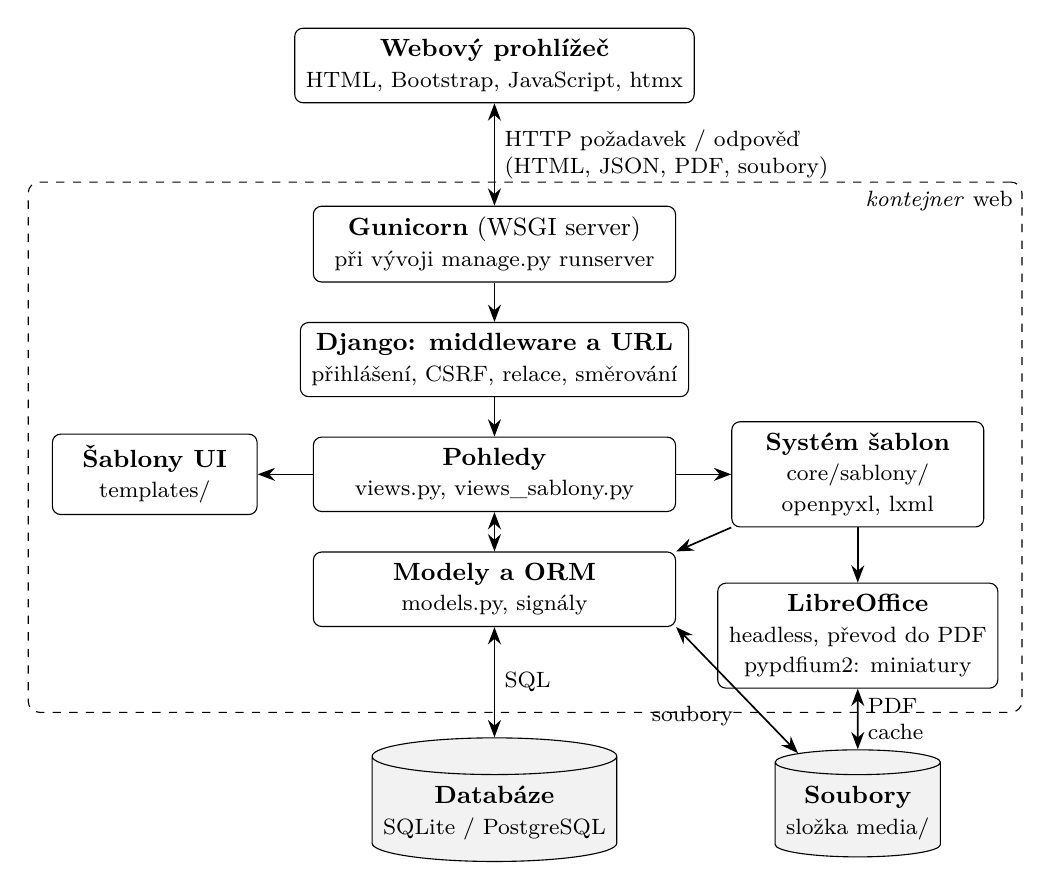
\begin{tikzpicture}[node distance=5mm and 7mm, font=\small]
  % klient
  \node[bm blok, minimum width=4.6cm] (prohlizec) {\textbf{Webový prohlížeč}\\\footnotesize HTML, Bootstrap, JavaScript, htmx};
  % kontejner web
  \node[bm blok, below=13mm of prohlizec, minimum width=4.6cm] (gunicorn) {\textbf{Gunicorn} (WSGI server)\\\footnotesize při vývoji \texttt{manage.py runserver}};
  \node[bm blok, below=of gunicorn, minimum width=4.6cm] (mw) {\textbf{Django: middleware a URL}\\\footnotesize přihlášení, CSRF, relace, směrování};
  \node[bm blok, below=of mw, minimum width=4.6cm] (views) {\textbf{Pohledy}\\\footnotesize \texttt{views.py}, \texttt{views\_sablony.py}};
  \node[bm blok, left=of views, minimum width=2.6cm] (tpl) {\textbf{Šablony UI}\\\footnotesize \texttt{templates/}};
  \node[bm blok, right=of views, minimum width=3.2cm] (sab) {\textbf{Systém šablon}\\\footnotesize \texttt{core/sablony/}\\\footnotesize openpyxl, lxml};
  \node[bm blok, below=of views, minimum width=4.6cm] (orm) {\textbf{Modely a ORM}\\\footnotesize \texttt{models.py}, signály};
  \node[bm blok, below=7mm of sab, minimum width=3.2cm] (lo) {\textbf{LibreOffice}\\\footnotesize headless, převod do PDF\\\footnotesize pypdfium2: miniatury};
  % data
  \node[bm uloziste, below=14mm of orm] (db) {\textbf{Databáze}\\\footnotesize SQLite / PostgreSQL};
  \node[bm uloziste] (media) at (db -| lo) {\textbf{Soubory}\\\footnotesize složka \texttt{media/}};
  % hranice kontejneru
  \begin{scope}[on background layer]
    \node[draw, dashed, rounded corners, inner sep=3mm, fit=(gunicorn) (tpl) (sab) (orm) (lo),
          label={[font=\footnotesize\itshape, anchor=north east]north east:kontejner \texttt{web}}] (web) {};
  \end{scope}
  % vazby
  \draw[bm obousmerna] (prohlizec) -- node[right, font=\footnotesize, align=left] {HTTP požadavek / odpověď\\(HTML, JSON, PDF, soubory)} (gunicorn);
  \draw[bm sipka] (gunicorn) -- (mw);
  \draw[bm sipka] (mw) -- (views);
  \draw[bm sipka] (views) -- (tpl);
  \draw[bm sipka] (views) -- (sab);
  \draw[bm obousmerna] (views) -- (orm);
  \draw[bm sipka] (sab) -- (lo);
  \draw[bm sipka] (sab.south west) -- (orm.north east);
  \draw[bm obousmerna] (orm) -- node[right, font=\footnotesize] {SQL} (db);
  \draw[bm obousmerna] (lo) -- node[right, font=\footnotesize, align=left] {PDF\\cache} (media);
  \draw[bm obousmerna] (orm.south east) -- node[pos=0.55, below left, font=\footnotesize] {soubory} (media.north west);
\end{tikzpicture}
\caption{Architektura aplikace BusinessManager}\label{fig:architektura}
\end{figure}

\paragraph{Frontend} tvoří HTML stránky, které server generuje ze šablon Django. Nejde o~samostatnou klientskou aplikaci (\emph{single-page application}), ale o~klasickou serverově vykreslovanou aplikaci: každé kliknutí nebo odeslání formuláře je běžný požadavek HTTP. Tento přístup je jednoduchý, spolehlivý a~celá logika zůstává na jednom místě.

\paragraph{Backend.} Požadavek přijme server Gunicorn, projde řetězcem \emph{middleware} (bezpečnost, relace, ochrana CSRF, průvodce prvním spuštěním, ověření přihlášení, kontrola oprávnění), URL směrování vybere pohled a~ten vrátí HTML stránku, data JSON nebo soubor. Většinu tabulek (číselníky, platby, kontaktní osoby) obsluhují \emph{obecné pohledy} pro seznam, detail, formulář a~smazání, které formulář vytvoří automaticky z~definice modelu. Hlavní agendy (nová zakázka, pracovní plocha, tvorba dokladů, kalendář) mají specializované pohledy. Doménová logika, která musí platit bez ohledu na to, odkud se data mění, je přímo v~modelech: číslování dokladů, výpočet cen a~součtů, kopie údajů zákazníka do dokladu. Zápis událostí do kalendáře zajišťují signály. Operace, které mění více tabulek najednou, probíhají v~databázové transakci.

\paragraph{Soubory} nahrané uživateli (fotografie, přílohy, šablony, logo) se ukládají do složky \texttt{media}, databáze obsahuje jen jejich cestu.

\paragraph{Zabezpečení.} Všechny stránky i~soubory jsou dostupné jen přihlášeným uživatelům. Formuláře jsou chráněny proti CSRF, výstupy šablon proti vložení kódu (XSS) a~dotazy do databáze skládá ORM bezpečně. Co smí který uživatel, určují role a~oprávnění. Oprávnění kontroluje middleware na serveru u~každého požadavku podle adresy, takže nestačí jen skrýt tlačítko; Nastavení a~šablony dokumentů vidí jen uživatel s~oprávněním Nastavení. Formuláře kontroluje server a~chybu hlásí česky u~políčka. Záznamy, na které navazuje historie, se nemažou, ale deaktivují. Hesla a~tajný klíč se nezapisují do zdrojového kódu, ale načítají se ze souboru \path{.env}.

\paragraph{Nasazení.} Ve firmě běží aplikace v~kontejnerech Docker (obrázek~\ref{fig:docker}). Kontejner \texttt{web} obsahuje aplikaci, LibreOffice a~písma, kontejner \texttt{db} databázi PostgreSQL, jejíž port není dostupný mimo Docker. Data jsou ve svazcích \texttt{pgdata} a~\texttt{media}, takže přežijí restart počítače i~aktualizaci aplikace. Při každém spuštění kontejner aplikuje migrace databáze a~po první instalaci se automaticky vytvoří výchozí data (stavy zakázek, oprávnění a~výchozí role, sazby DPH, vestavěné šablony). Instalaci, aktualizaci a~zálohování zajišťují skripty \path{instalace.bat}, \path{aktualizace.bat} a~\path{zaloha.bat}; postup popisuje oddíl~\ref{sec:nasazeni} a~instalační návod v~repozitáři. Při vývoji lze aplikaci spustit i~bez Dockeru nad databází SQLite. Podrobný popis vrstev, složek se soubory, komunikace komponent a~spuštění je v~dokumentaci aplikace\footnote{\url{https://github.com/MajkyyQ/BusinessManager/blob/main/docs/04-architektura.md}}.

\begin{figure}[htbp]
\centering
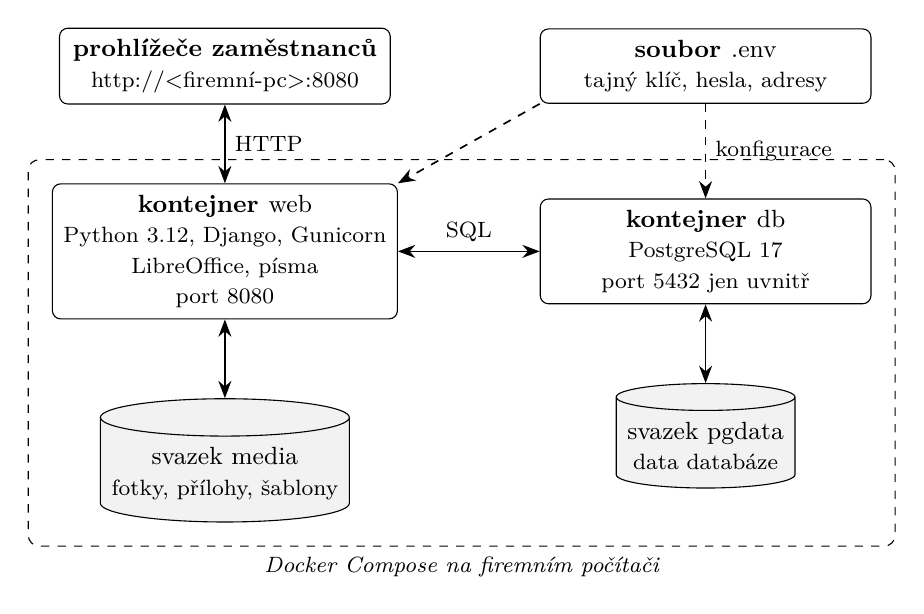
\begin{tikzpicture}[node distance=6mm and 10mm, font=\small]
  \node[bm blok, minimum width=4.2cm] (web) {\textbf{kontejner \texttt{web}}\\\footnotesize Python 3.12, Django, Gunicorn\\\footnotesize LibreOffice, písma\\\footnotesize port 8080};
  \node[bm blok, right=18mm of web, minimum width=4.2cm] (dbk) {\textbf{kontejner \texttt{db}}\\\footnotesize PostgreSQL 17\\\footnotesize port 5432 jen uvnitř};
  \node[bm uloziste, below=10mm of web] (vmedia) {svazek \texttt{media}\\\footnotesize fotky, přílohy, šablony};
  \node[bm uloziste, below=10mm of dbk] (vpg) {svazek \texttt{pgdata}\\\footnotesize data databáze};
  \node[bm blok, above=10mm of web, minimum width=4.2cm] (pc) {\textbf{prohlížeče zaměstnanců}\\\footnotesize \texttt{http://<firemní-pc>:8080}};
  \node[bm blok, minimum width=4.2cm] (env) at (pc -| dbk) {\textbf{soubor \texttt{.env}}\\\footnotesize tajný klíč, hesla, adresy};
  \begin{scope}[on background layer]
    \node[draw, dashed, rounded corners, inner sep=3mm, fit=(web) (dbk) (vmedia) (vpg),
          label={[font=\footnotesize\itshape, anchor=north]south:Docker Compose na firemním počítači}] {};
  \end{scope}
  \draw[bm obousmerna] (pc) -- node[right, font=\footnotesize] {HTTP} (web);
  \draw[bm obousmerna] (web) -- node[above, font=\footnotesize] {SQL} (dbk);
  \draw[bm obousmerna] (web) -- (vmedia);
  \draw[bm obousmerna] (dbk) -- (vpg);
  \draw[bm sipka, dashed] (env) -- node[right, font=\footnotesize] {konfigurace} (dbk);
  \draw[bm sipka, dashed] (env.south west) -- (web.north east);
\end{tikzpicture}
\caption{Nasazení aplikace pomocí Docker Compose}\label{fig:docker}
\end{figure}

% ============================================================
% Struktura projektu (zkrácená verze; úplný popis je v dokumentaci
% aplikace: docs/05-struktura-projektu.md v repozitáři)
% ============================================================
\section{Struktura projektu}\label{sec:struktura-projektu}

Zdrojový kód je uspořádán podle konvencí frameworku Django. Projekt tvoří konfigurační balíček \path{config} a~jediná aplikace \path{core}, která obsahuje veškerou funkcionalitu. Rozdělení do více aplikací Django nebylo pro rozsah projektu potřebné; logické části jsou místo toho odděleny do modulů (modely, pohledy evidence, pohledy šablon, číslování dokladů) a~do samostatného balíčku \path{core/sablony/} se systémem šablon dokumentů, který na pohledech nezávisí. Závislosti mezi moduly tak směřují jedním směrem, což odpovídá vrstvené architektuře z~předchozího oddílu. Strom souborů s~popisem každé složky je součástí dokumentace aplikace\footnote{\url{https://github.com/MajkyyQ/BusinessManager/blob/main/docs/05-struktura-projektu.md}}.

% ============================================================
% Databáze (zkrácená verze; popis všech tabulek a sloupců je v dokumentaci
% aplikace: docs/07-databaze.md a docs/databaze-tabulky.md v repozitáři)
% ============================================================
\section{Databázový model}\label{sec:databaze}

Aplikace ukládá data do relační databáze. Relační model byl zvolen, protože data mají pevnou strukturu a~jsou navzájem silně provázaná: zakázka patří zákazníkovi, obsahuje jeho zařízení a~navazují na ni práce, materiál, doklady a~platby. Vazby vyjadřují cizí klíče a~databáze hlídá jejich platnost, takže nemůže vzniknout například zakázka bez zákazníka. Podporovány jsou systémy SQLite (vývoj, provoz bez Dockeru) a~PostgreSQL~17 (provoz ve firmě); kód aplikace je pro oba stejný.

Databáze je jediným místem, kde jsou uložena data aplikace. Soubory (fotografie, přílohy, šablony, logo) se do ní neukládají, obsahuje jen jejich cestu. Výsledné dokumenty se také neukládají, ale vždy se sestavují z~aktuálních dat. Aplikace s~databází pracuje výhradně přes ORM frameworku Django: každá tabulka je popsána modelem v~souboru \path{core/models.py} a~z~modelů vznikají migrace, které schéma vytvoří nebo upraví. Pro návrh jsou důležité tyto konvence:

\begin{itemize}
\item Každá tabulka má primární klíč \texttt{id}, cizí klíče se ukládají do sloupců s~příponou \texttt{\_id} a~u~každého je určeno chování při smazání odkazovaného záznamu (\texttt{PROTECT}, \texttt{CASCADE}, \texttt{SET\_NULL}). Databáze sama hlídá, aby cizí klíč neodkazoval na neexistující záznam (viz oddíl~\ref{sec:principy-odchylky}).
\item Vazby M:N realizují vazební tabulky se dvěma cizími klíči, například \path{core_zakazka_zarizeni}.
\item Peněžní částky se ukládají jako desetinná čísla s~pevnou přesností (\texttt{DecimalField}), aby nevznikaly zaokrouhlovací chyby. Datum a~čas se ukládá v~UTC.
\item Záznamy číselníků a~evidence mají sloupec \texttt{aktivni}; smazání v~aplikaci je jen deaktivace, takže historické zakázky a~doklady zůstávají úplné.
\item Schéma obsahuje kromě klíčů i~omezení \texttt{UNIQUE} a~\texttt{CHECK} (tabulka~\ref{tab:principy-omezeni}). Formuláře je kontrolují už před uložením a~zobrazí srozumitelné hlášení.
\end{itemize}

\subsection{Schéma databáze}\label{sec:schema-databaze}

Databáze obsahuje 30~tabulek aplikace a~10~vazebních tabulek pro vazby M:N. Navíc aplikace využívá tabulku uživatelských účtů \path{auth_user} frameworku Django. Schéma je rozděleno do tří obrázků: jádro databáze se zakázkou (obrázek~\ref{fig:db-zakazka}), doklady, platby, přijaté faktury a~kalendář (obrázek~\ref{fig:db-doklady}) a~uživatelé, oprávnění a~nastavení (obrázek~\ref{fig:db-ostatni}). Popisky na spojnicích udávají kardinalitu vazby.

\begin{figure}[htbp]
\centering
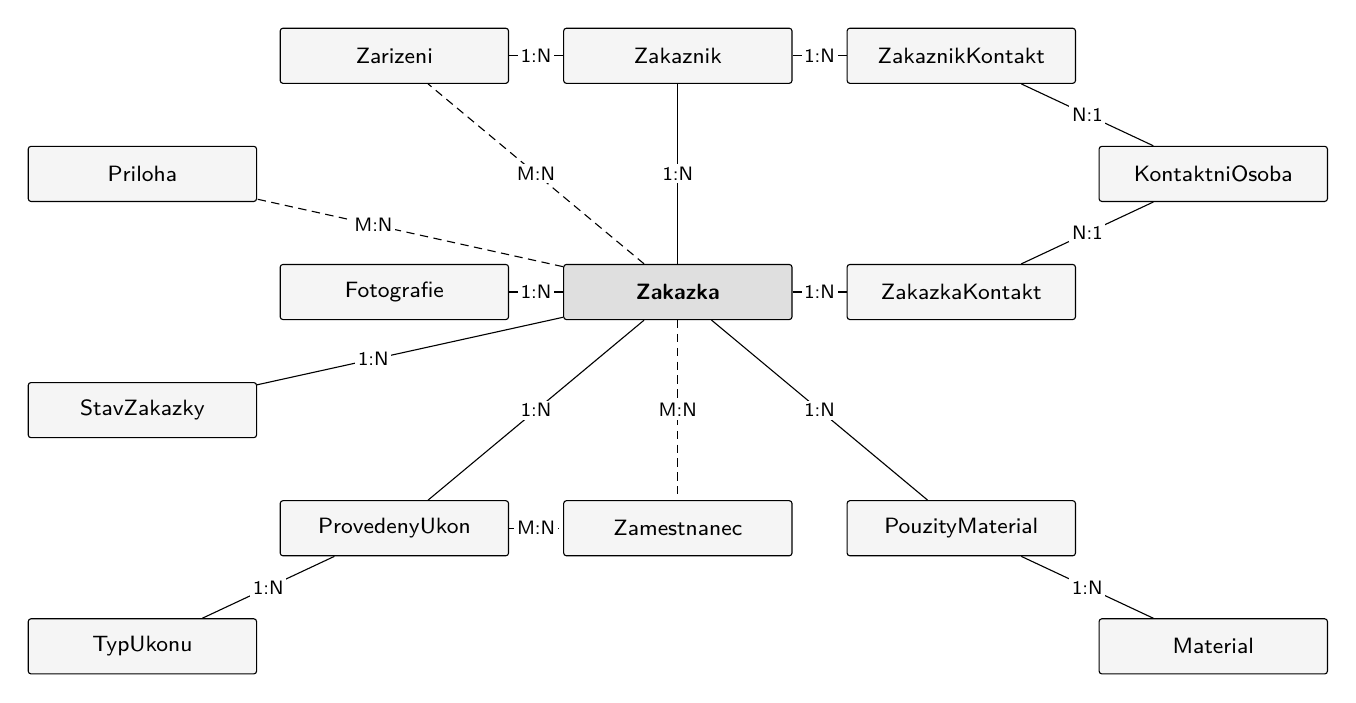
\begin{tikzpicture}[x=1cm, y=1cm]
  \node[bm tabulka, fill=gray!25, font=\footnotesize\sffamily\bfseries] (zakazka) at (6.8,-3) {Zakazka};
  \node[bm tabulka] (zakaznik) at (6.8,0) {Zakaznik};
  \node[bm tabulka] (zarizeni) at (3.2,0) {Zarizeni};
  \node[bm tabulka] (zkontakt) at (10.4,0) {ZakaznikKontakt};
  \node[bm tabulka] (kosoba) at (13.6,-1.5) {KontaktniOsoba};
  \node[bm tabulka] (zakkontakt) at (10.4,-3) {ZakazkaKontakt};
  \node[bm tabulka] (foto) at (3.2,-3) {Fotografie};
  \node[bm tabulka] (priloha) at (0,-1.5) {Priloha};
  \node[bm tabulka] (stav) at (0,-4.5) {StavZakazky};
  \node[bm tabulka] (ukon) at (3.2,-6) {ProvedenyUkon};
  \node[bm tabulka] (typukonu) at (0,-7.5) {TypUkonu};
  \node[bm tabulka] (zam) at (6.8,-6) {Zamestnanec};
  \node[bm tabulka] (pmat) at (10.4,-6) {PouzityMaterial};
  \node[bm tabulka] (mat) at (13.6,-7.5) {Material};

  \draw (zakaznik) -- node[bm vazba] {1:N} (zarizeni);
  \draw (zakaznik) -- node[bm vazba] {1:N} (zakazka);
  \draw (zakaznik) -- node[bm vazba] {1:N} (zkontakt);
  \draw (zkontakt) -- node[bm vazba] {N:1} (kosoba);
  \draw (zakazka) -- node[bm vazba] {1:N} (zakkontakt);
  \draw (zakkontakt) -- node[bm vazba] {N:1} (kosoba);
  \draw[densely dashed] (zakazka) -- node[bm vazba] {M:N} (zarizeni);
  \draw (zakazka) -- node[bm vazba] {1:N} (foto);
  \draw[densely dashed] (zakazka) -- node[bm vazba, pos=0.62] {M:N} (priloha);
  \draw (stav) -- node[bm vazba, pos=0.38] {1:N} (zakazka);
  \draw (zakazka) -- node[bm vazba] {1:N} (ukon);
  \draw[densely dashed] (zakazka) -- node[bm vazba] {M:N} (zam);
  \draw (zakazka) -- node[bm vazba] {1:N} (pmat);
  \draw (typukonu) -- node[bm vazba] {1:N} (ukon);
  \draw[densely dashed] (ukon) -- node[bm vazba] {M:N} (zam);
  \draw (mat) -- node[bm vazba] {1:N} (pmat);
\end{tikzpicture}
\caption{Schéma databáze -- zakázka a navázané tabulky (čárkovaně vazby M:N)}\label{fig:db-zakazka}
\end{figure}

\begin{figure}[htbp]
\centering
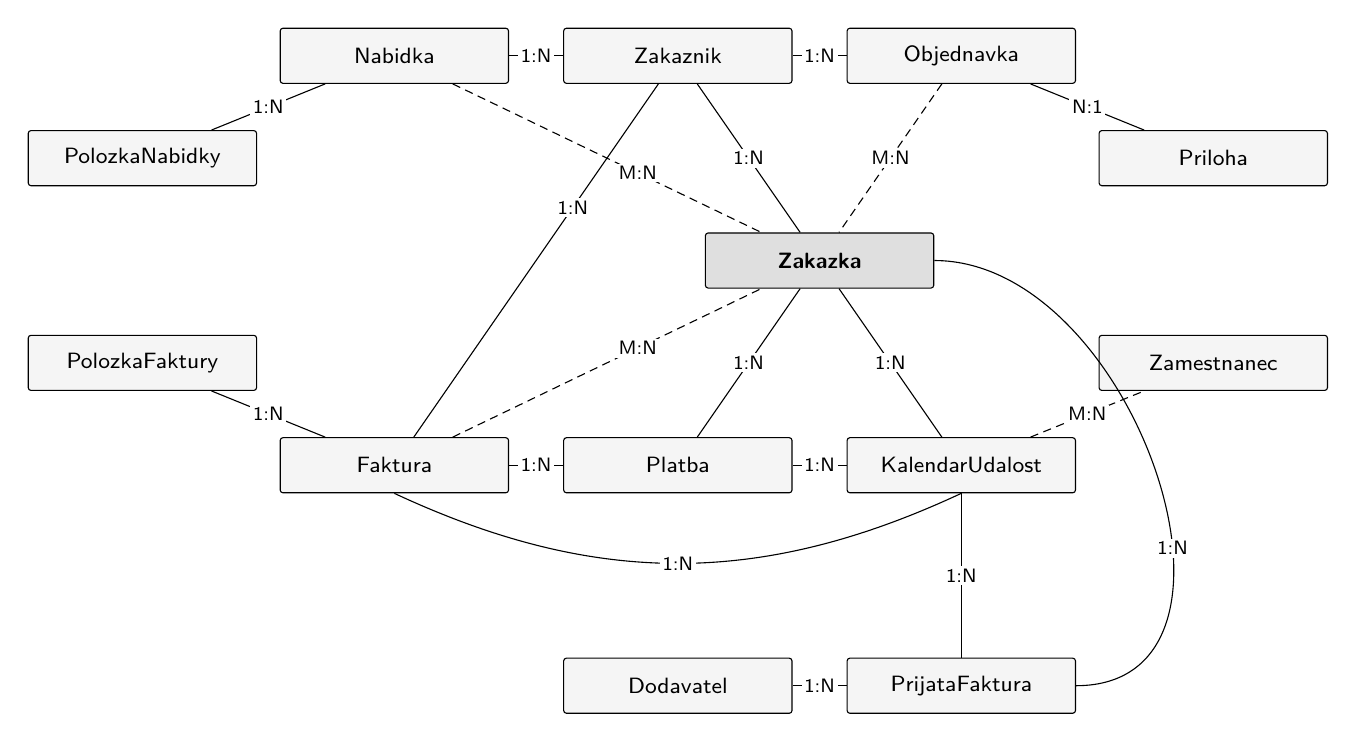
\begin{tikzpicture}[x=1cm, y=1cm]
  \node[bm tabulka] (zakaznik) at (6.8,0) {Zakaznik};
  \node[bm tabulka, fill=gray!25, font=\footnotesize\sffamily\bfseries] (zakazka) at (8.6,-2.6) {Zakazka};
  \node[bm tabulka] (nabidka) at (3.2,0) {Nabidka};
  \node[bm tabulka] (pnab) at (0,-1.3) {PolozkaNabidky};
  \node[bm tabulka] (objed) at (10.4,0) {Objednavka};
  \node[bm tabulka] (priloha) at (13.6,-1.3) {Priloha};
  \node[bm tabulka] (faktura) at (3.2,-5.2) {Faktura};
  \node[bm tabulka] (pfak) at (0,-3.9) {PolozkaFaktury};
  \node[bm tabulka] (platba) at (6.8,-5.2) {Platba};
  \node[bm tabulka] (kal) at (10.4,-5.2) {KalendarUdalost};
  \node[bm tabulka] (zam) at (13.6,-3.9) {Zamestnanec};
  \node[bm tabulka] (prijata) at (10.4,-8.0) {PrijataFaktura};
  \node[bm tabulka] (dodavatel) at (6.8,-8.0) {Dodavatel};

  \draw (zakaznik) -- node[bm vazba] {1:N} (nabidka);
  \draw (zakaznik) -- node[bm vazba] {1:N} (objed);
  \draw (zakaznik) -- node[bm vazba, pos=0.35] {1:N} (faktura);
  \draw (zakaznik) -- node[bm vazba] {1:N} (zakazka);
  \draw (nabidka) -- node[bm vazba] {1:N} (pnab);
  \draw (faktura) -- node[bm vazba] {1:N} (pfak);
  \draw[densely dashed] (nabidka) -- node[bm vazba, pos=0.6] {M:N} (zakazka);
  \draw[densely dashed] (objed) -- node[bm vazba] {M:N} (zakazka);
  \draw[densely dashed] (faktura) -- node[bm vazba, pos=0.6] {M:N} (zakazka);
  \draw (objed) -- node[bm vazba] {N:1} (priloha);
  \draw (faktura) -- node[bm vazba] {1:N} (platba);
  \draw (zakazka) -- node[bm vazba] {1:N} (platba);
  \draw (platba) -- node[bm vazba] {1:N} (kal);
  \draw (zakazka) -- node[bm vazba] {1:N} (kal);
  \draw (faktura.south) to[out=-25, in=-155] node[bm vazba] {1:N} (kal.south);
  \draw[densely dashed] (kal) -- node[bm vazba] {M:N} (zam);
  \draw (prijata) -- node[bm vazba] {1:N} (kal);
  \draw (dodavatel) -- node[bm vazba] {1:N} (prijata);
  \draw (zakazka.east) to[out=0, in=0, looseness=1.15] node[bm vazba, pos=0.62] {1:N} (prijata.east);
\end{tikzpicture}
\caption{Schéma databáze -- doklady, platby, přijaté faktury a kalendář}\label{fig:db-doklady}
\end{figure}

\begin{figure}[htbp]
\centering
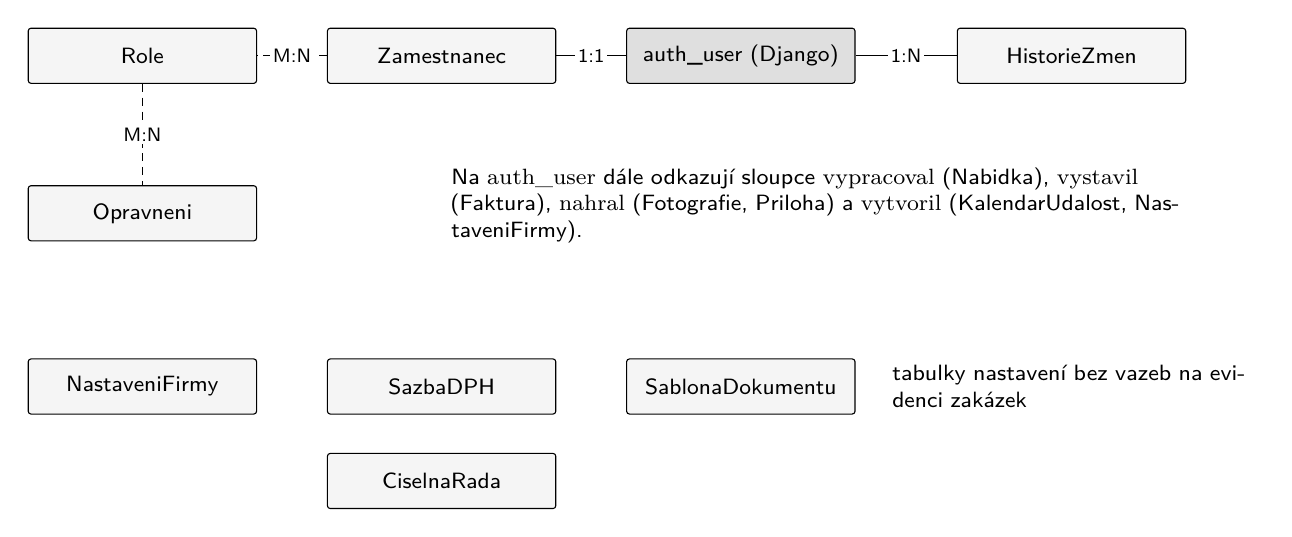
\begin{tikzpicture}[x=1cm, y=1cm]
  \node[bm tabulka, fill=gray!25] (user) at (7.6,0) {auth\_user (Django)};
  \node[bm tabulka] (zam) at (3.8,0) {Zamestnanec};
  \node[bm tabulka] (role) at (0,0) {Role};
  \node[bm tabulka] (opr) at (0,-2) {Opravneni};
  \node[bm tabulka] (hist) at (11.8,0) {HistorieZmen};
  \node[font=\footnotesize\sffamily, align=left, text width=9.2cm, anchor=north west] (pozn) at (3.8,-1.3)
     {Na \texttt{auth\_user} dále odkazují sloupce \texttt{vypracoval} (Nabidka), \texttt{vystavil} (Faktura), \texttt{nahral} (Fotografie, Priloha) a~\texttt{vytvoril} (KalendarUdalost, NastaveniFirmy).};
  \node[bm tabulka] (nast) at (0,-4.2) {NastaveniFirmy};
  \node[bm tabulka] (dph) at (3.8,-4.2) {SazbaDPH};
  \node[bm tabulka] (sab) at (7.6,-4.2) {SablonaDokumentu};
  \node[bm tabulka] (cis) at (3.8,-5.4) {CiselnaRada};
  \node[font=\footnotesize\sffamily, align=left, text width=4.6cm, anchor=west] at (9.4,-4.2) {tabulky nastavení bez vazeb na evidenci zakázek};

  \draw (user) -- node[bm vazba] {1:1} (zam);
  \draw[densely dashed] (zam) -- node[bm vazba] {M:N} (role);
  \draw[densely dashed] (role) -- node[bm vazba] {M:N} (opr);
  \draw (user) -- node[bm vazba] {1:N} (hist);
\end{tikzpicture}
\caption{Schéma databáze -- uživatelé, oprávnění a nastavení}\label{fig:db-ostatni}
\end{figure}
\subsection{Klíčové části modelu}\label{sec:tabulky}

\paragraph{Zakázka} (tabulka Zakazka) je středem celého modelu. Odkazuje na zákazníka a~na stav z~číselníku StavZakazky a~nese číslo zakázky, datum přijetí a~vydání a~popis závady. Se zařízeními a~zaměstnanci je spojena vazbami M:N, s~kontaktními osobami tabulkou ZakazkaKontakt, která nese roli osoby (například \enquote{přinesl zařízení}). Na zakázku navazují fotografie, přílohy, provedené práce (ProvedenyUkon) a~použitý materiál (PouzityMaterial). Použitý materiál si při uložení zkopíruje aktuální cenu z~katalogu, takže pozdější změna ceníku starší zakázky neovlivní.

\paragraph{Doklady.} Nabídka a~faktura mají vlastní tabulky položek (PolozkaNabidky, PolozkaFaktury) a~kromě odkazu na zákazníka obsahují i~\emph{kopii jeho údajů} (jméno, firmu, adresu, IČO a~DIČ) v~okamžiku vystavení. Pozdější změna adresy zákazníka tak vystavený doklad nezmění. Toto zdvojení údajů je záměrnou odchylkou od normalizace, kterou zdůvodňuje oddíl~\ref{sec:principy-odchylky}. Každá položka si při uložení spočítá cenu bez DPH a~s~DPH a~přepočítá součty dokladu. Podobu čísel dokladů určuje tabulka CiselnaRada. K~faktuře se váže platba (Platba).

\paragraph{Kalendář a historie.} Tabulka KalendarUdalost uchovává ruční i~automatické události (přijetí a~vydání zakázky, vystavení a~zaplacení faktury, splatnost přijaté faktury), které vznikají signály modelů. Tabulka HistorieZmen zaznamenává, kdo, kdy a~co v~aplikaci změnil.

\paragraph{Přijaté faktury} od dodavatelů eviduje tabulka PrijataFaktura spolu s~číselníkem dodavatelů (Dodavatel). Nejsou součástí dokladů firmy, ale přehledu jejích závazků.

\paragraph{Nastavení a~oprávnění.} Tabulky nastavení nemají vazby na evidenci zakázek a~obsahují údaje o~firmě (NastaveniFirmy, včetně odkazu na účet, který firmu založil), sazby DPH, číselné řady a~šablony dokumentů (SablonaDokumentu). Barvu a~pořadí stavů zakázky ukládá číselník StavZakazky. Tabulky Role a~Opravneni určují, co smí který zaměstnanec: zaměstnanci se přiřadí role a~role je svazek oprávnění. Šablona obsahuje jen vzhled dokumentu a~mapování polí ve formátu JSON, nikdy jeho data.

Popis všech tabulek s~účelem, sloupci, datovými typy, klíči a~integritními omezeními je součástí dokumentace aplikace\footnote{\url{https://github.com/MajkyyQ/BusinessManager/blob/main/docs/07-databaze.md}}. Úplný referenční přehled sloupců se generuje přímo z~modelů aplikace\footnote{\url{https://github.com/MajkyyQ/BusinessManager/blob/main/docs/databaze-tabulky.md}}, takže vždy odpovídá aktuální verzi.

% Praktická část: porovnání databáze aplikace s principy z kapitoly kap:principy-db.
% Vkládá se do kapitoly 07-navrh.tex.
\section{Databázový model a~jeho soulad s~principy návrhu}\label{sec:db-soulad}

Tento oddíl porovnává databázi aplikace s~principy z~kapitoly~\ref{kap:principy-db}. U~každého principu uvádí, jak se v~návrhu uplatnil, a~na konci popisuje místa, kde se návrh od doporučení knihy záměrně odchyluje. Konkrétní tabulky a~sloupce popisuje oddíl~\ref{sec:databaze}.

\subsection{Klíče}

V~souladu s~doporučením má v~aplikaci každá tabulka umělý primární klíč \texttt{id}, celé číslo generované databází. Údaje, které uživatelé používají k~vyhledání záznamu, jako číslo zakázky, číslo faktury nebo číslo nabídky, jsou uloženy jako samostatné sloupce s~omezením \texttt{UNIQUE}. Jsou to tedy kandidátní klíče, ale ne primární klíče. Uživatel je může změnit, aniž by se musely měnit odkazy z~jiných tabulek. Všechny vazby mezi tabulkami jsou v~aplikaci vyjádřeny cizími klíči a~databáze nedovolí uložit odkaz na neexistující záznam. Například zakázku nelze přiřadit neexistujícímu zákazníkovi.

\subsection{E-R model a~převod na tabulky}

V~aplikaci jsou zastoupeny všechny druhy kardinality:
\begin{itemize}
\item \textbf{1:N} -- zákazník má více zařízení a~více zakázek, každé zařízení a~každá zakázka patří právě jednomu zákazníkovi (úplná účast zakázky);
\item \textbf{N:1 s~částečnou účastí} -- zakázka může, ale nemusí mít přiřazený stav;
\item \textbf{M:N} -- zakázka zahrnuje více zařízení a~jedno zařízení může být opravováno v~několika zakázkách; obdobně zakázky a~zaměstnanci nebo faktury a~zakázky;
\item \textbf{1:1} -- zaměstnanec má nejvýše jeden uživatelský účet a~účet patří nejvýše jednomu zaměstnanci.
\end{itemize}

Slabými entitami jsou v~aplikaci položky nabídek a~faktur: položka bez dokladu neexistuje a~při smazání dokladu se smaže i~ona. Nabídka a~faktura sdílejí zákazníka, kopii jeho údajů, částky a~vazbu na zakázky; společné atributy jsou proto popsány jednou, v~obecném dokladu. Podmínka disjunktní a~úplné generalizace platí, protože každý doklad je buď nabídka, nebo faktura. Aplikace proto podle druhé metody převodu má samostatné tabulky Nabidka a~Faktura a~stejně tak PolozkaNabidky a~PolozkaFaktury.

Databáze aplikace je vytvořena přesně podle pravidel převodu z~oddílu~\ref{sec:principy-er}. Vztahy N:1 jsou cizí klíče, například \texttt{zakaznik\_id} v~tabulce Zakazka. Vztahy M:N mají vazební tabulky, například \path{core_zakazka_zarizeni}. Vztahy s~popisnými atributy mají vlastní tabulku: ZakaznikKontakt nese poznámku ke kontaktní osobě a~ZakazkaKontakt roli osoby na zakázce, například \enquote{přinesl zařízení}. Vazební tabulky mají kvůli frameworku Django vlastní sloupec \texttt{id}, a~proto mají nad dvojicí cizích klíčů omezení \texttt{UNIQUE}. Stejná kontaktní osoba tak nemůže být u~jednoho zákazníka uvedena dvakrát. Zákazník proto nemá sloupec se seznamem svých zařízení. Vztah je uložen jen jednou, cizím klíčem v~tabulce Zarizeni.

\subsection{Normalizace}

Tabulky aplikace neobsahují množinové atributy. Vícehodnotové údaje, například zařízení na zakázce, jsou uloženy ve vazebních tabulkách. Výjimky z~1NF jsou popsány v~oddílu~\ref{sec:principy-odchylky}. Kniha uvádí, že pečlivě navržený E-R model vede ke schématu, které další normalizaci nepotřebuje \cite[s.~344]{Silberschatz2020}. To se u~aplikace potvrdilo. Údaje, které by se jinak opakovaly, jsou ve vlastních tabulkách -- číselnících: stavy zakázek, typy úkonů, materiál a~sazby DPH. Zakázka tak neukládá název stavu, ale jen odkaz na řádek tabulky StavZakazky. Přejmenování stavu se proto projeví u~všech zakázek najednou. V~tabulkách zákazníků, zařízení, zakázek a~číselníků určuje všechny ostatní atributy jen primární klíč, případně kandidátní klíč (číslo zakázky). Tyto tabulky jsou tedy v~BCNF. Na tomto principu stojí kopie údajů zákazníka na vystavených dokladech (oddíl~\ref{sec:principy-odchylky}).

\subsection{Integritní omezení}

Tabulka~\ref{tab:principy-omezeni} ukazuje, jak jsou tato omezení použita v~aplikaci. Omezení jsou deklarována v~modelech a~Django je převádí do databázového schématu. Formuláře aplikace je kontrolují už před uložením, takže uživatel dostane srozumitelné hlášení místo chyby databáze.

\begin{longtable}{p{0.20\textwidth}p{0.72\textwidth}}
\caption{Integritní omezení v~databázi aplikace}\label{tab:principy-omezeni}\\
\hline \textbf{Druh omezení} & \textbf{Použití v~aplikaci} \\ \hline\endfirsthead
\hline \textbf{Druh omezení} & \textbf{Použití v~aplikaci} \\ \hline\endhead
PRIMARY KEY & sloupec \texttt{id} v~každé tabulce \\
UNIQUE & číslo zakázky, nabídky a~faktury; druh dokladu v~číselné řadě; kód oprávnění; dvojice (dodavatel, číslo faktury dodavatele); dvojice (zákazník, kontaktní osoba); trojice (zakázka, kontaktní osoba, role) \\
NOT NULL & cizí klíče s~úplnou účastí (zákazník zakázky, zařízení a~dokladu), názvy v~číselnících, popis položky dokladu \\
CHECK -- výčet & typ zákazníka, role kontaktní osoby, stav a~způsob platby, stav přijaté faktury, typ události kalendáře, měna, druh dokladu a~způsob nulování číselné řady \\
CHECK --\newline podmínka & zákazník musí mít vyplněné jméno nebo firmu; sazba DPH v~rozsahu 0--100~\%; datum zaplacení přijaté faktury jen u~zaplacené faktury \\
FOREIGN KEY & všechny vazby mezi tabulkami; chování při smazání PROTECT (odmítnutí), CASCADE (např. položky dokladu) nebo SET NULL \\
\hline
\end{longtable}

\subsection{Datové typy}

Aplikace se řídí doporučeními knihy k~datovým typům:
\begin{itemize}
\item \textbf{Peněžní částky} jsou typu \texttt{numeric(12,2)}.
\item \textbf{Texty} jsou typu \texttt{varchar(n)} s~maximální délkou.
\item \textbf{Datum a~čas}: údaje, u~kterých záleží jen na dni (splatnost, datum zdanitelného plnění), jsou typu \texttt{date}. Okamžiky, například vytvoření záznamu nebo přijetí zakázky, jsou typu \texttt{timestamp} s~časovým pásmem.
\item \textbf{Soubory} (fotografie, přílohy, šablony) se do databáze jako typ \texttt{blob} neukládají, i~když to kniha umožňuje. Ukládají se do souborového systému a~databáze obsahuje jen cestu k~souboru. Databáze tak zůstává malá a~zálohu souborů lze dělat zvlášť.
\end{itemize}

Pro rychlé vyhledávání mají indexy sloupce, podle kterých uživatelé hledají, například sériové číslo zařízení a~identifikační číslo zakázky. Cizí klíče dostávají index automaticky. Tabulky aplikace mají české názvy v~jednotném čísle a~vazební tabulky se jmenují spojením názvů propojených tabulek, například \path{core_zakazka_zarizeni}.

\subsection{Objektově-relační mapování a~aplikační logika}

Aplikace nepracuje s~databází přímo pomocí SQL, ale přes \emph{objektově-relační mapování} (ORM) frameworku Django. Model v~souboru \path{core/models.py} je tedy zároveň definicí relačního schématu a~všechna omezení z~tabulky~\ref{tab:principy-omezeni} jsou zapsána v~něm. Část pravidel aplikace hlídá ve vrstvě aplikační logiky. Patří sem například kontrolní součet IČO nebo automatické vytváření událostí kalendáře. Změny dat zaznamenává tabulka HistorieZmen.

\subsection{Ochrana proti SQL injection}\label{sec:db-sql-injection}

Aplikace obě doporučení z~oddílu~\ref{sec:principy-sql-injection} splňuje:
\begin{itemize}
\item Všechny dotazy vytváří Django ORM (oddíl~\ref{sec:principy-orm}), které hodnoty předává databázi vždy jako parametry dotazu \cite{django-security}. V~kódu aplikace se nepoužívá žádné ručně psané SQL.
\item Přihlášení zajišťuje vestavěný modul Djanga. Uživatel se vyhledá podle jména parametrizovaným dotazem a~heslo se v~databázi vůbec nehledá.
\item Seznam zakázek lze řadit podle sloupce zvoleného v~adrese stránky. Název sloupce se do dotazu nepřipojuje přímo, ale vybírá se z~pevného seznamu povolených sloupců. Neznámá hodnota se nahradí výchozím řazením podle čísla zakázky.
\end{itemize}

Hesla se v~databázi neukládají jako text. Django přesně takto postupuje a~ve výchozím nastavení používá algoritmus PBKDF2 s~hašovací funkcí SHA-256 a~náhodnou solí \cite{django-hesla}. Omezení znaků, které smí uživatel zadat do jména nebo hesla, se jako ochrana proti SQL injection nepoužívá. Přihlašovací jméno je omezené jen tím, co povoluje Django: písmena, číslice a~znaky \texttt{@~.~+~-~\_}.

Odolnost aplikace ověřují automatické testy (třída \texttt{SQLInjectionTest} v~souboru \path{core/tests.py}). Testy zkoušejí přihlášení s~devíti typickými útočnými řetězci, například \texttt{' OR '1'='1}, \texttt{admin'-{}-} nebo \texttt{'; DROP TABLE auth\_user; -{}-}, ve jménu, v~hesle i~v~obou polích zároveň. Žádný pokus uživatele nepřihlásí a~tabulka uživatelů zůstane beze změny. Testy dále ověřují, že heslo obsahující uvozovky a~pomlčky funguje jako běžné heslo a~že útočné řetězce ve vyhledávání ani v~parametru řazení nevrátí cizí data ani nezpůsobí chybu. Testy prošly v~databázi SQLite i~PostgreSQL.

\section{Odchylky od doporučení a~jejich zdůvodnění}\label{sec:principy-odchylky}

Návrh databáze se na několika místech od doporučení knihy odchyluje. Každá odchylka je záměrná: doporučený postup by buď omezil funkce aplikace, nebo by si vyžádal rozsáhlé změny bez odpovídajícího přínosu. Tabulka~\ref{tab:principy-odchylky} shrnuje odchylky, podrobnější zdůvodnění následuje.

\begin{longtable}{p{0.27\textwidth}p{0.27\textwidth}p{0.38\textwidth}}
\caption{Odchylky návrhu od doporučení knihy}\label{tab:principy-odchylky}\\
\hline \textbf{Řešení v~aplikaci} & \textbf{Doporučení knihy} & \textbf{Důvod odchylky} \\ \hline\endfirsthead
\hline \textbf{Řešení v~aplikaci} & \textbf{Doporučení knihy} & \textbf{Důvod odchylky} \\ \hline\endhead
kopie údajů zákazníka na dokladu & bez redundance (s.~303--304) & doklad musí zachytit stav v~den vystavení (s.~347--348) \\
uložené součty dokladu a~ceny položek & odvozený atribut se neukládá (s.~251) & vystavená částka se nesmí měnit, rychlé přehledy (s.~346) \\
uložená cena použitého materiálu & bez redundance & historická cena se nesmí měnit se změnou ceníku \\
číslo dokladu obsahuje rok a~pořadí & atomické domény, 1NF (s.~342) & formát čísla si určuje firma, číslo se zobrazuje i~tiskne celé \\
adresa v~jednom sloupci & složený atribut (s.~250, 342) & adresy se zadávají volně, rozklad potřebuje jen export ISDOC \\
platba odkazuje na fakturu i~zakázku & bez redundantních vztahů (s.~261--262) & platba může existovat i~bez faktury \\
události kalendáře s~kopií data & odvozený údaj se neukládá & kalendář obsahuje i~ruční události a~události bez dokladu \\
pořadové číslo dokladu z~existujících čísel & čítač nebo sekvence (s.~160--161) & pořadí závisí na formátu a~období, jedinečnost zajišťuje UNIQUE \\
historie změn bez cizího klíče & referenční integrita (s.~149) & záznam musí přežít smazání objektu (s.~445) \\
kontrolní součet IČO jen v~aplikaci & omezení ve schématu (s.~146) & výpočet nelze zapsat podmínkou CHECK, IČO z~ISDOC nemusí být platné \\
nepovinná cena položky a~nejednotné typy datumů & NOT NULL (s.~146), typ podle významu (s.~154) & textové položky bez ceny, nabídka a~platba evidují i~čas \\
\hline
\end{longtable}

\subsection{Kopie údajů zákazníka na dokladu}

Nabídka a~faktura obsahují kromě odkazu na zákazníka i~kopii jeho jména, firmy, adresy, IČO a~DIČ. Údaje jsou tak uloženy dvakrát, což je redundance, před kterou kniha varuje \cite[s.~303--304]{Silberschatz2020}. Jde ale o~časově proměnná data. Funkční závislost \enquote{zákazník $\rightarrow$ adresa} platí jen pro aktuální stav, ne pro celou historii \cite[s.~347--348]{Silberschatz2020}. Vystavený doklad musí i~po letech obsahovat údaje platné v~den vystavení. Kdyby se četly z~tabulky zákazníků, změna adresy by zpětně změnila všechny vystavené faktury. Kniha pro takové údaje navrhuje doplnit k~záznamům období platnosti \cite[s.~348]{Silberschatz2020}. Pro doklad, který se po vystavení nemění, je jednodušší a~srozumitelnější uložit kopii. Ze stejného důvodu se při použití materiálu na zakázce kopíruje jeho aktuální cena. Pozdější změna ceníku tak nezmění cenu na již provedených zakázkách.

\subsection{Uložené součty a~ceny}

Cena položky dokladu (množství krát jednotková cena) a~součty dokladu jsou odvozené atributy. Kniha uvádí, že odvozený atribut se obvykle neukládá, ale počítá se při použití \cite[s.~251]{Silberschatz2020}. V~aplikaci se součty ukládají ze dvou důvodů. Částka vystavené faktury je účetní údaj a~nesmí se změnit, ani kdyby se později změnil způsob zaokrouhlení. Přehledy dokladů navíc zobrazují částky bez nutnosti načítat všechny položky. Jde o~denormalizaci, kterou kniha připouští, pokud aplikace udržuje redundantní údaje v~souladu \cite[s.~346]{Silberschatz2020}. Aplikace to zajišťuje přepočtem součtů při každém uložení položky.

\subsection{Struktura čísel dokladů}

Podobu čísel zakázek, nabídek a~faktur si firma určí sama v~nastavení aplikace. Administrátor napíše ukázkové číslo, například \texttt{Fa260001}, a~aplikace v~něm pozná rok, měsíc, den a~pořadové číslo. Vzor uloží do tabulky CiselnaRada jako formát se značkami, například \texttt{Fa\{YY\}\{N4\}}. Dokud firma řadu nezmění, platí dosavadní tvary \texttt{RRRR-NNN} pro zakázku a~nabídku a~\texttt{NNN-DD-MM/RRRR} pro fakturu (například 001-27-10/2026). Hotové číslo dokladu tedy obsahuje rok a~pořadí. Podle knihy takové hodnoty nemají atomickou doménu a~schéma s~nimi formálně není v~1NF. Kniha uvádí, že informace je pak zakódována v~programu místo v~databázi \cite[s.~342--343]{Silberschatz2020}. Formát čísla je ale v~aplikaci uložen v~databázi a~rozklad čísla se používá jen na jednom místě, při generování nového čísla (modul \path{core/cislovani.py}). Jinak je číslo atomickým identifikátorem: zobrazuje se, tiskne a~vyhledává vždy celé. Uživatel navíc může zadat vlastní číslo, které formátu odpovídat nemusí, a~vystavené doklady si svá čísla ponechají i~po změně formátu. Rozdělení do samostatných sloupců by vyžadovalo změnu tiskových šablon a~exportu ISDOC a~přineslo by dvě kopie stejné informace. Proto zůstává číslo v~jednom sloupci.

Pořadí nového čísla se počítá z~existujících čísel: aplikace najde nejvyšší pořadí v~daném období a~přičte jedna. Kniha upozorňuje, že prohledávání existujících hodnot je pomalé, a~doporučuje čítač v~samostatné tabulce nebo sekvenci databáze \cite[s.~160--161]{Silberschatz2020}. Sekvence ale nezná formát čísla a~neumí začínat od jedné každý rok nebo měsíc podle nastavení firmy. Čítač by se navíc musel opravovat při každém ručně zadaném nebo smazaném čísle. Jedinečnost čísla zajišťuje omezení \texttt{UNIQUE} a~aplikace obsazená čísla přeskočí, takže ani při současném uložení dvou dokladů nemůže vzniknout duplicita. V~nejhorším případě aplikace ohlásí chybu a~uživatel doklad uloží znovu. U~malé firmy s~několika zaměstnanci je taková situace velmi nepravděpodobná.

\subsection{Adresa jako jeden údaj}

Adresa je podle knihy \emph{složený atribut} (ulice, město, PSČ) \cite[s.~250]{Silberschatz2020}. Kniha doporučuje rozdělit ho do samostatných sloupců, pokud aplikace pracuje s~jednotlivými částmi \cite[s.~342]{Silberschatz2020}. Aplikace adresu ukládá jako jeden text. Uživatelé ji zadávají ve tvaru, v~jakém se tiskne na doklady, a~jednotlivé části potřebuje jen export faktury do formátu ISDOC. Ten adresu rozdělí podle čárek a~PSČ a~nerozpoznanou část ponechá, aby se údaj neztratil. Rozdělení adresy do sloupců by změnilo všechny formuláře a~tiskové šablony. Proto je ponecháno jako možné budoucí rozšíření.

\subsection{Vazby platby a~událostí kalendáře}

Platba má cizí klíč na fakturu i~na zakázku. Pokud je platba vázaná na fakturu, je zakázka odvoditelná z~faktury a~údaj je redundantní \cite[s.~261--262]{Silberschatz2020}. Platba ale může vzniknout i~bez faktury, například při zaplacení drobné opravy v~hotovosti. Odkaz na zakázku je proto nutný.

Události kalendáře se vytvářejí automaticky při přijetí zakázky, vystavení faktury nebo zaplacení. Obsahují kopii data a~odkaz na zakázku nebo doklad. Datum by šlo odvodit z~dokladu, ale kalendář musí v~jednom seznamu zobrazit i~ruční události a~události bez dokladu. Kopie se při každé změně zakázky nebo faktury aktualizuje. Kniha k~takovým automatickým akcím, které odpovídají triggerům, doporučuje opatrnost \cite[s.~213]{Silberschatz2020}. Aplikace je proto drží jednoduché: každá akce jen vytvoří nebo upraví jednu událost a~nespouští další akce.

\subsection{Historie změn bez cizího klíče}

Tabulka HistorieZmen ukládá typ objektu a~jeho \texttt{id}, ale nemá na objekt cizí klíč. Databáze tedy referenční integritu této vazby nehlídá. Je to záměrné: auditní záznam musí uchovat i~informaci o~smazání objektu \cite[s.~445]{Silberschatz2020}. Cizí klíč by smazání buď zakázal, nebo by smazal i~záznam historie. Sloupec \texttt{id\_objektu} má stejný datový typ jako primární klíče, jak kniha požaduje u~odkazujících sloupců \cite[s.~149]{Silberschatz2020}.

\subsection{Pravidla kontrolovaná aplikací}

Některá omezení nejsou v~databázi, ale jen v~aplikaci. Kontrolní součet IČO nelze rozumně zapsat podmínkou \texttt{CHECK} \cite[s.~147]{Silberschatz2020}. Údaje dodavatele z~importovaného souboru ISDOC navíc nemusí být platné, a~aplikace je musí umět uložit a~nechat uživatele je opravit. Kontrolu proto provádí validátor ve formuláři.

Cena položky dokladu může zůstat prázdná. Kniha doporučuje omezení NOT NULL u~atributů, u~kterých prázdná hodnota nemá smysl \cite[s.~146]{Silberschatz2020}. Položky se do dokladu převezmou ze zakázky, v~detailu dokladu je ale lze upravit, takže na dokladu může zůstat i~textová položka bez ceny, například poznámka k~rozsahu opravy.

Datum vystavení nabídky a~datum zaplacení platby jsou uloženy včetně času, zatímco datum vystavení faktury jen jako datum. Kniha doporučuje volit typ podle významu údaje \cite[s.~154]{Silberschatz2020}. Faktura podle zákona o~DPH nese jen datum. Čas nabídky a~platby se zobrazuje v~kalendáři a~v~historii zakázky.

\subsection{Ochrana při mazání v~aplikační vrstvě}

Chování při smazání odkazovaného záznamu (PROTECT, CASCADE, SET NULL) určuje v~aplikaci Django, nikoli klauzule \texttt{ON DELETE} v~databázi. Django ve verzi 5.2 vytváří cizí klíče bez této klauzule a~kaskádové mazání nebo jeho odmítnutí provede samo před odesláním příkazu do databáze. Databáze přesto hlídá referenční integritu: neplatný odkaz by odmítla. Výsledek je stejný, jaký kniha popisuje pro \texttt{ON DELETE CASCADE} a~odmítnutí operace \cite[s.~149--150]{Silberschatz2020}. Rozdíl je jen v~tom, kdo akci provádí.

% Praktická část: porovnání rozhraní aplikace s doporučeními z kapitoly
% kap:uzivatelske-rozhrani. Vkládá se do kapitoly 07-navrh.tex.
% Stav odpovídá aplikaci k 23. 11. 2026 (po PR #69).
\section{Návrh uživatelského rozhraní a~jeho soulad se zásadami}\label{sec:ui-soulad}

Tento oddíl porovnává rozhraní aplikace se zásadami z~kapitoly~\ref{kap:uzivatelske-rozhrani}. U~každého návrhového rozhodnutí uvádí, o~které doporučení se opírá a~zda ho aplikace splňuje. Úpravy, které porovnání vyvolalo, popisuje konec oddílu.

\subsection{Rozvržení obrazovky}

Obrazovka aplikace má tři pevné části. Nahoře je lišta s~logem a~názvem aplikace, přepínačem světlého a~tmavého režimu, jménem přihlášeného uživatele a~tlačítkem pro odhlášení. Vlevo je svislá navigace s~hlavními částmi aplikace: Pracovní plocha, Zakázky, Zákazníci, Zařízení, Dokumenty, Kalendář a~(jen pro uživatele s~oprávněním Nastavení) Nastavení. Zbytek obrazovky zabírá obsah zvolené části. Nad obsahem je drobečková navigace, která ukazuje, kde se uživatel nachází.

Svislá navigace vlevo odpovídá doporučení Laubheimera: svislý seznam se rychle prohlíží a~lze do něj přidávat další položky \cite{Laubheimer2021}. To je pro aplikaci důležité, protože každý nový modul přidá do navigace novou položku. Navigaci lze sbalit jen na ikony, což Laubheimer připouští u~aplikací používaných denně. Ve výchozím stavu jsou proto vidět ikony i~textové popisky.

\subsection{Přehled rozhodnutí}

Tabulka~\ref{tab:ui-soulad} shrnuje hlavní rozhodnutí o~rozhraní a~jejich oporu v~literatuře.

\begin{longtable}{p{0.34\textwidth}p{0.40\textwidth}p{0.16\textwidth}}
\caption{Rozhodnutí o~uživatelském rozhraní a~jejich opora}\label{tab:ui-soulad}\\
\hline \textbf{Rozhodnutí} & \textbf{Opora} & \textbf{Stav} \\ \hline\endfirsthead
\hline \textbf{Rozhodnutí} & \textbf{Opora} & \textbf{Stav} \\ \hline\endhead
Hlavní menu je svislá lišta vlevo s~ikonou a~textem & svislá navigace vlevo se snadno prohlíží a~rozšiřuje \cite{Laubheimer2021} & splňuje \\
Lištu lze sbalit jen na ikony & přijatelné u~aplikací používaných denně \cite{Laubheimer2021} & splňuje \\
Tlačítko \enquote{+ Nový} je u~všech seznamů na stejném místě vpravo nahoře & hlavní akce na stejném místě v~pravém horním rohu \cite{Kaplan2021}; konzistence \cite[s.~2328]{Sajedi2011}; Fittsův zákon \cite[s.~2330]{Sajedi2011} & splňuje \\
Všechny seznamy mají stejnou tabulku, hledání a~řazení & konzistence \cite{Nielsen-heuristiky}, \cite{Shneiderman-pravidla}, \cite[s.~2328]{Sajedi2011} & splňuje \\
Postup v~aplikaci kopíruje postup ve firmě & shoda s~reálným světem \cite{Nielsen-heuristiky}; cyklus událostí \cite[s.~56]{MonkWagner2013} & splňuje \\
Nabídka a~faktura se skládají z~uložených dat zakázky & faktura vzniká kopírováním dat objednávky \cite[s.~57]{MonkWagner2013}; systém doplňuje známé údaje \cite[s.~2331--2332]{Sajedi2011} & splňuje \\
Vše o~zakázce na jedné obrazovce se záložkami & snížit zátěž krátkodobé paměti \cite{Shneiderman-pravidla}; jednoduché propojené formuláře \cite[s.~2330]{Sajedi2011} & splňuje \\
Výběr zákazníka, zařízení a~materiálu našeptávačem s~možností založit nový záznam & prevence chyb, rozpoznání místo vybavování \cite{Nielsen-heuristiky} & splňuje \\
Pracovní plocha s~naposledy otevřenými a~otevřenými zakázkami & rozpoznání místo vybavování \cite{Nielsen-heuristiky}; systém si pamatuje volby \cite[s.~2331--2332]{Sajedi2011} & splňuje \\
Drobečková navigace a~zvýrazněná položka menu & viditelnost stavu systému \cite{Nielsen-heuristiky}; navigace \cite[s.~2332--2333]{Sajedi2011} & splňuje \\
Hlášení po uložení nebo smazání & informativní zpětná vazba \cite{Shneiderman-pravidla} & splňuje \\
Záznamy s~historií se jen deaktivují, změny se zapisují do historie & snadné vrácení akcí \cite{Shneiderman-pravidla}; nouzový východ \cite[s.~2331]{Sajedi2011} & splňuje \\
Nastavení a~šablony vidí jen uživatel s~oprávněním Nastavení, ostatní tlačítka se skrývají podle role & postupné odhalování \cite{Nielsen-progressive}; skrýt funkce podle oprávnění \cite[s.~2331]{Sajedi2011} & splňuje \\
Stav zakázky má barvu (volitelnou v~nastavení) i~text & barva jen jako doplněk \cite[s.~2329]{Sajedi2011}; WCAG 1.4.1 \cite{WCAG22} & splňuje \\
Aplikace obsahuje jen funkce, které firma potřebuje & minimalistický design \cite{Nielsen-heuristiky}; skrýt informace navíc \cite[s.~2332]{Sajedi2011} & splňuje \\
Na stránce zakázky je zvýrazněn jeden doporučený další krok, ostatní tlačítka jsou ve skupinách & minimalismus a~hierarchie \cite{Nielsen-heuristiky}, \cite{Kaplan2021}; dialogy s~jasným zakončením \cite{Shneiderman-pravidla} & splňuje \\
Nápověda u~složitějších formulářů & nápověda \cite[s.~2330]{Sajedi2011}, \cite{Nielsen-heuristiky} & splňuje \\
Kontrast textu a~velikost klikacích prvků & WCAG 1.4.3 a~2.5.8 \cite{WCAG22} & splňuje \\
Nevratné akce se potvrzují v~okně aplikace s~jasnou otázkou a~pojmenovaným tlačítkem & předcházet chybám \cite{Shneiderman-pravidla}; potvrzení nevratné akce \cite[s.~2331--2332]{Sajedi2011} & splňuje \\
Chybný údaj ve formuláři se hlásí česky u~políčka s~příkladem správného zápisu & pomoc s~rozpoznáním a~opravou chyb \cite{Nielsen-heuristiky} & splňuje \\
\hline
\end{longtable}

\subsection{Inspirace z~rešerše}\label{sec:ui-inspirace}

Při návrhu seznamů aplikace byly využity podněty z~rešerše (oddíl~\ref{sec:reserse-inspirace}). Všechny vycházejí z~požadavku na konzistenci rozhraní \cite{Nielsen-heuristiky}, \cite[s.~2328]{Sajedi2011}, který rešerše potvrdila: jednotné rozložení obrazovky bylo pozitivně hodnoceno u~Odoo i~ABRA Flexi.

\paragraph{Jednotné rozložení seznamů.} Všechny sekce mají stejnou hlavičku: vlevo název a~počet záznamů, vpravo hlavní akce. Pod ní je lišta, ve které je vyhledávací pole vždy na prvním místě a~ve stejné šířce, za ním filtry a~vpravo přepínač zobrazení. Sloupce tabulky mají pevnou šířku, takže se po filtrování ani hledání nepřeskupí a~uživatel nemusí znovu hledat, kde je který údaj.

\paragraph{Okno Filtrovat a~souhrn dokladů.} Seznam zakázek, seznam zařízení a~kalendář mají vedle vyhledávacího pole tlačítko \enquote{Filtrovat} (obrázek~\ref{obr:bm-filtr-stavu}). Otevře okno, ve kterém uživatel zaškrtne, co chce vidět: stavy s~počtem záznamů v~každém z~nich (u~zařízení stav jejich poslední zakázky), v~kalendáři typy událostí a~zaměstnance. U~zakázek v~něm zvolí i~řazení podle data přijetí nebo vydání. Tlačítko ukazuje počet zvolených filtrů a~vedle něj jsou štítky aktivních filtrů, které lze jedním kliknutím odebrat, takže je stále vidět, co je vyfiltrováno \cite{Nielsen-heuristiky}. Sekce Dokumenty má nad tabulkou řádek typů dokumentů s~počty, mezi kterými se přepíná jako mezi záložkami. Pod tabulkou dokumentů je navíc souhrn počtu a~celkové částky dokladů, inspirovaný ABRA Flexi.

\paragraph{Kanbanové zobrazení (Odoo).} Seznam zákazníků, zařízení a~zakázek lze přepnout z~tabulky na karty (obrázky~\ref{obr:odoo-prepinac} a~\ref{obr:bm-kanban}). Karta obsahuje jen základní údaje, podobně jako kanban kontaktů v~Odoo. Zakázky jsou v~kanbanu rozdělené do sloupců podle stavu, takže je na první pohled vidět, kolik práce čeká v~jaké fázi. Aplikace si zvolené zobrazení pamatuje zvlášť pro každý seznam.

\begin{figure}[h]
\centering
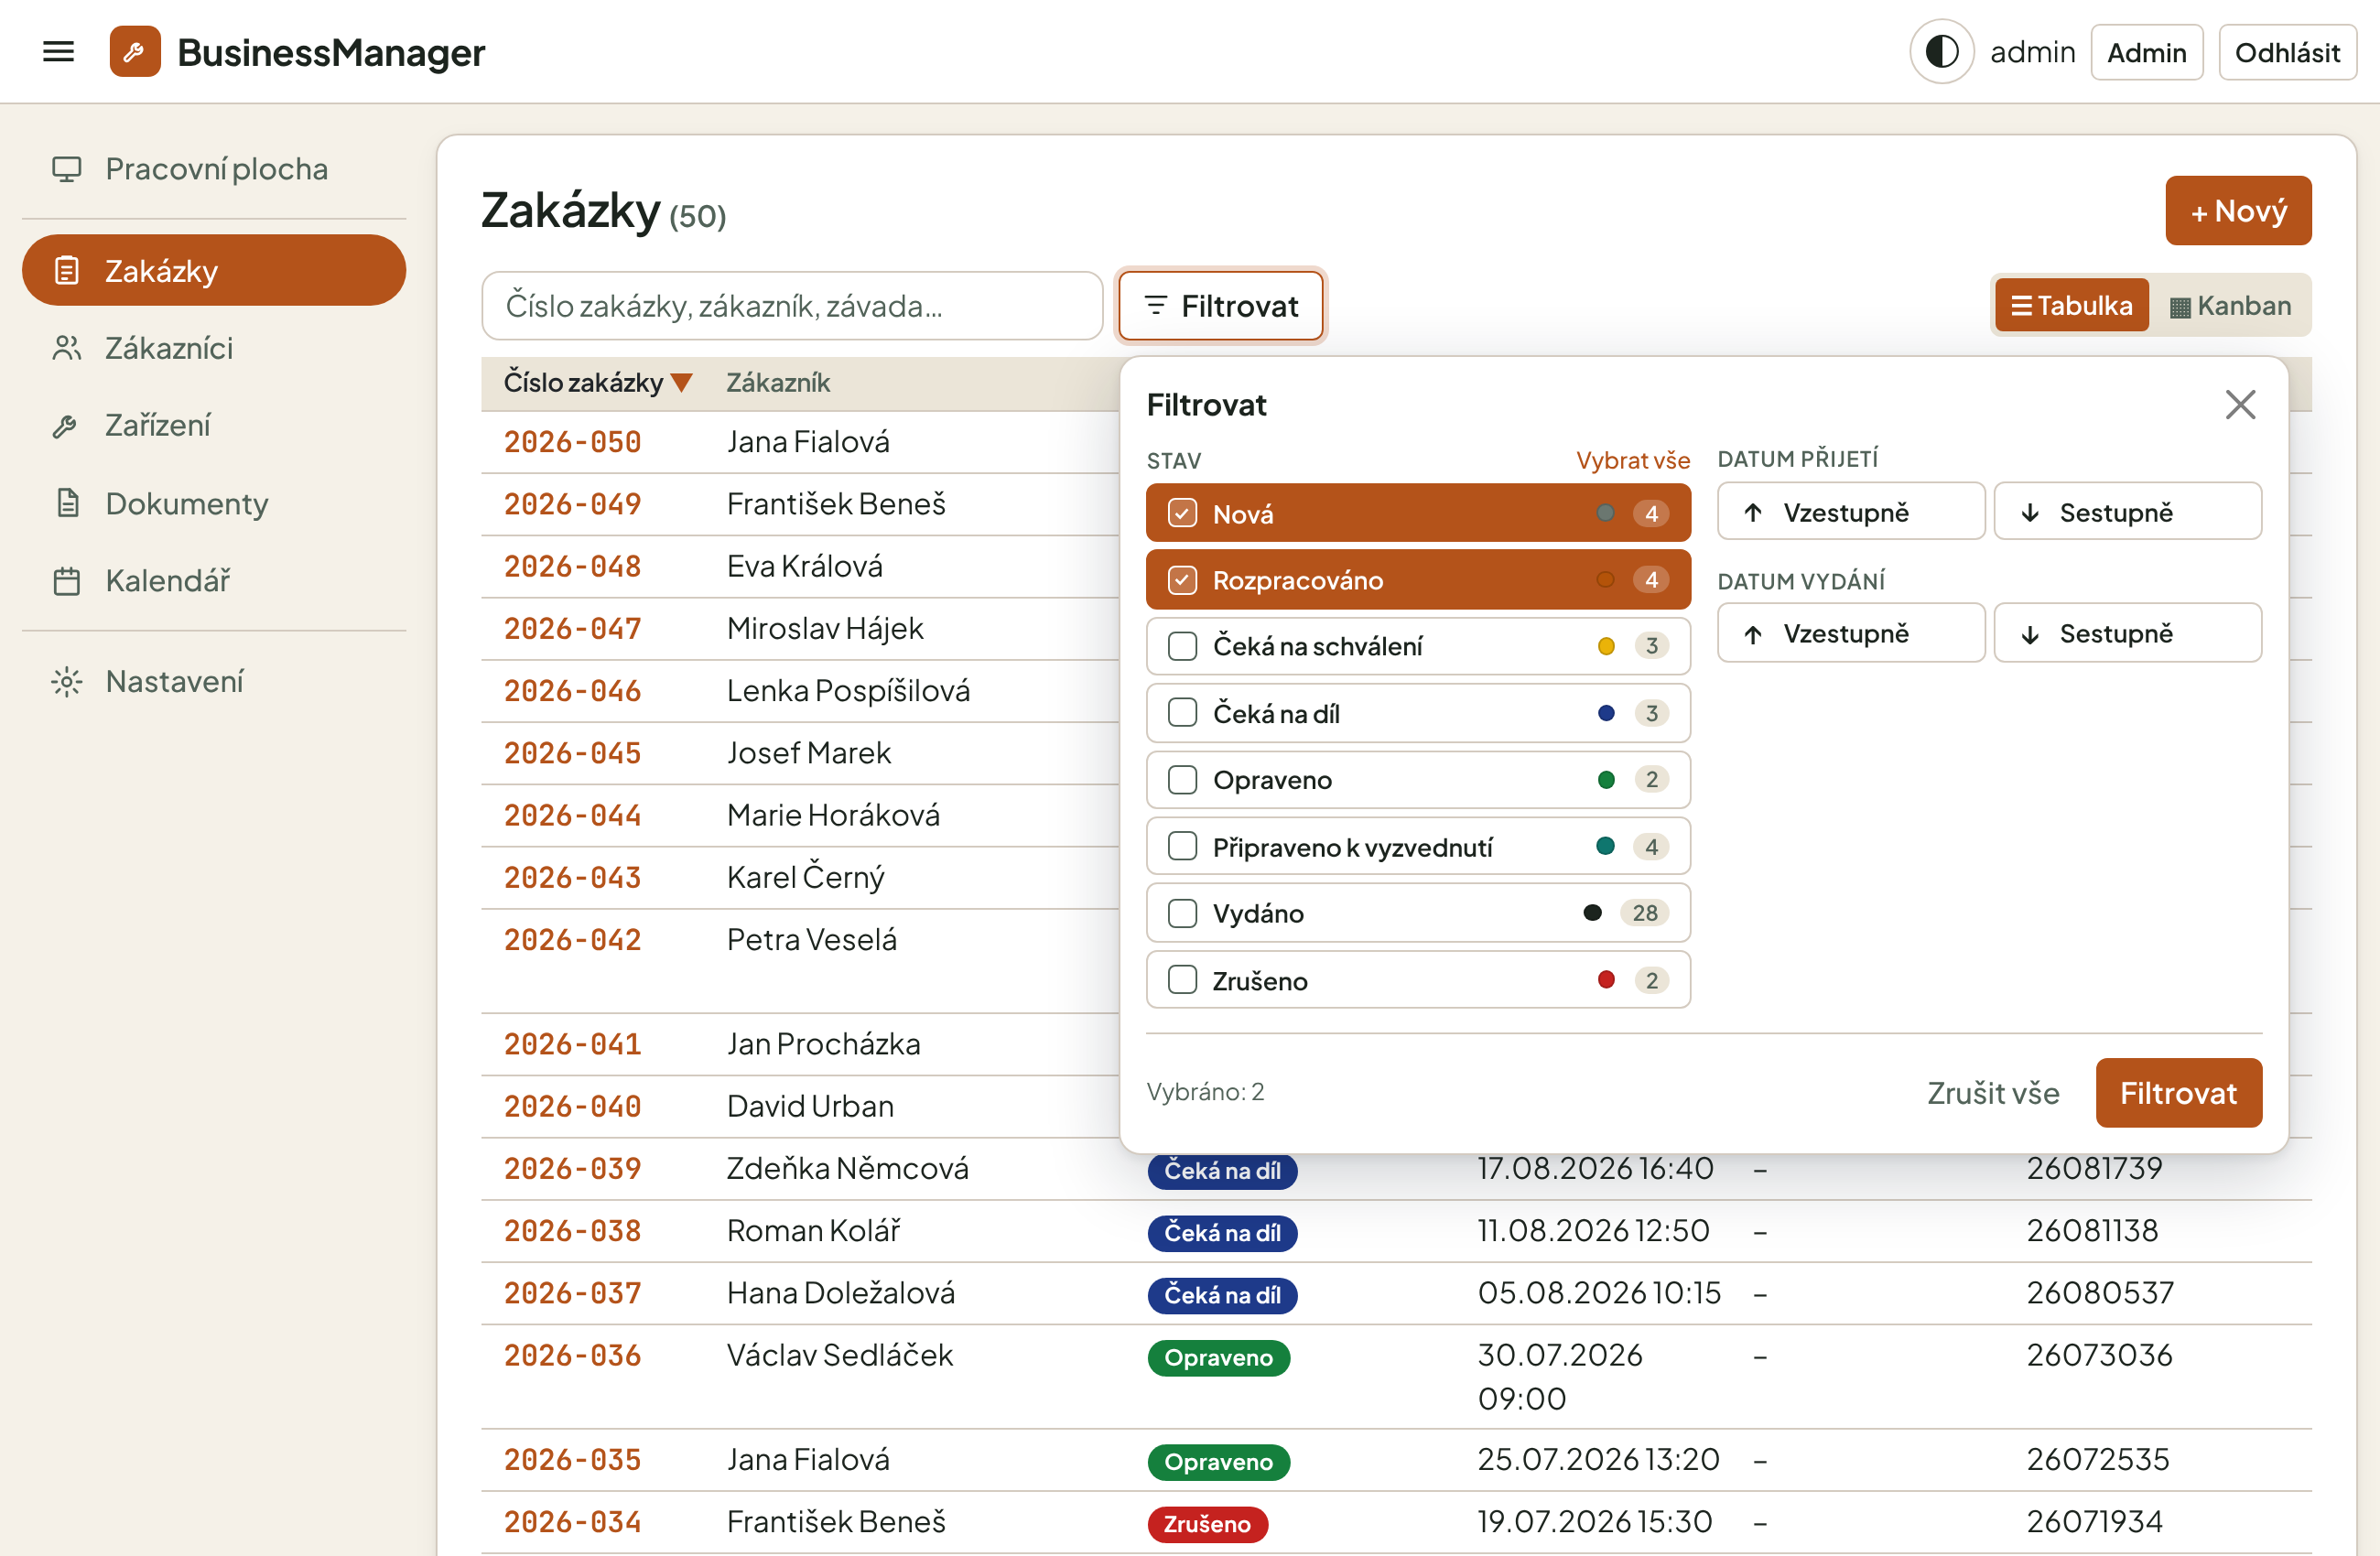
\includegraphics[width=\linewidth]{obrazky/navrh/bm-zakazky-filtr.png}
\caption{Seznam zakázek v~aplikaci s~otevřeným oknem Filtrovat, stavy s~počty záznamů a~řazením podle data (zdroj: vlastní)}\label{obr:bm-filtr-stavu}
\end{figure}

\begin{figure}[h]
\centering
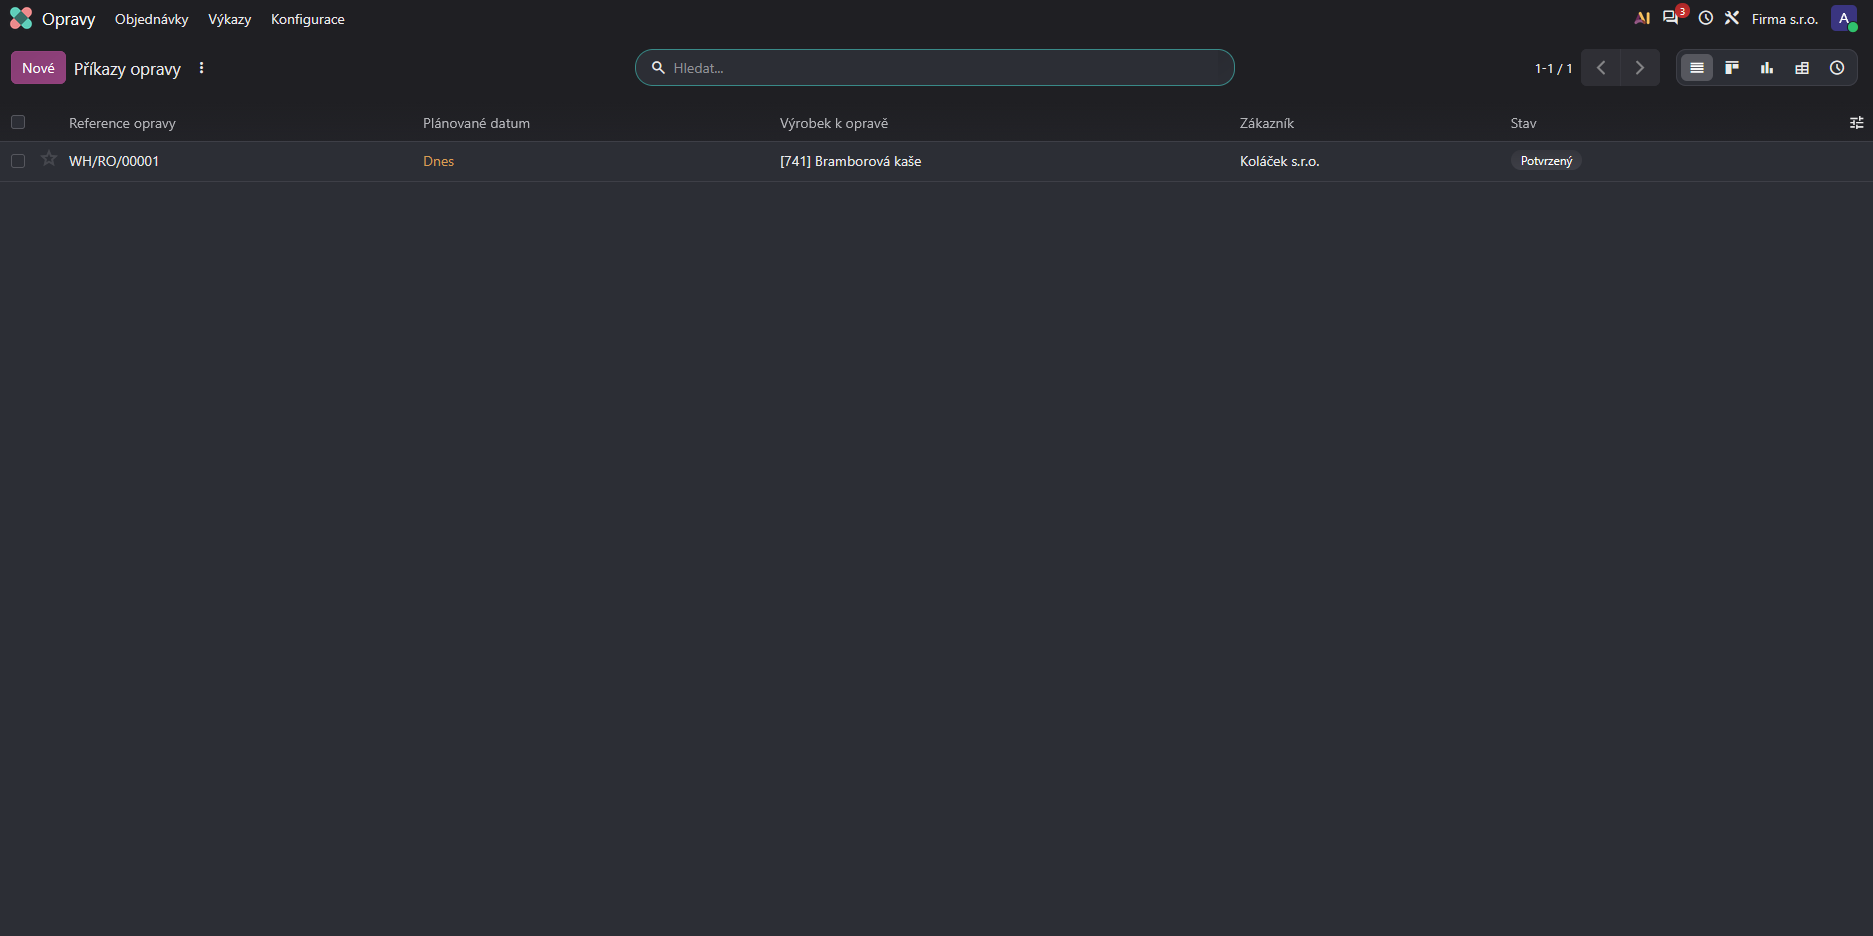
\includegraphics[width=\linewidth]{obrazky/reserse/odoo_strana_opravy.png}
\caption{Seznam oprav v~Odoo s~přepínačem zobrazení vpravo nahoře (seznam, kanban, graf, pivot, aktivity) (zdroj: vlastní snímek obrazovky ze zkušební verze, pořízeno 3.~11.~2026)}\label{obr:odoo-prepinac}
\end{figure}

\begin{figure}[h]
\centering
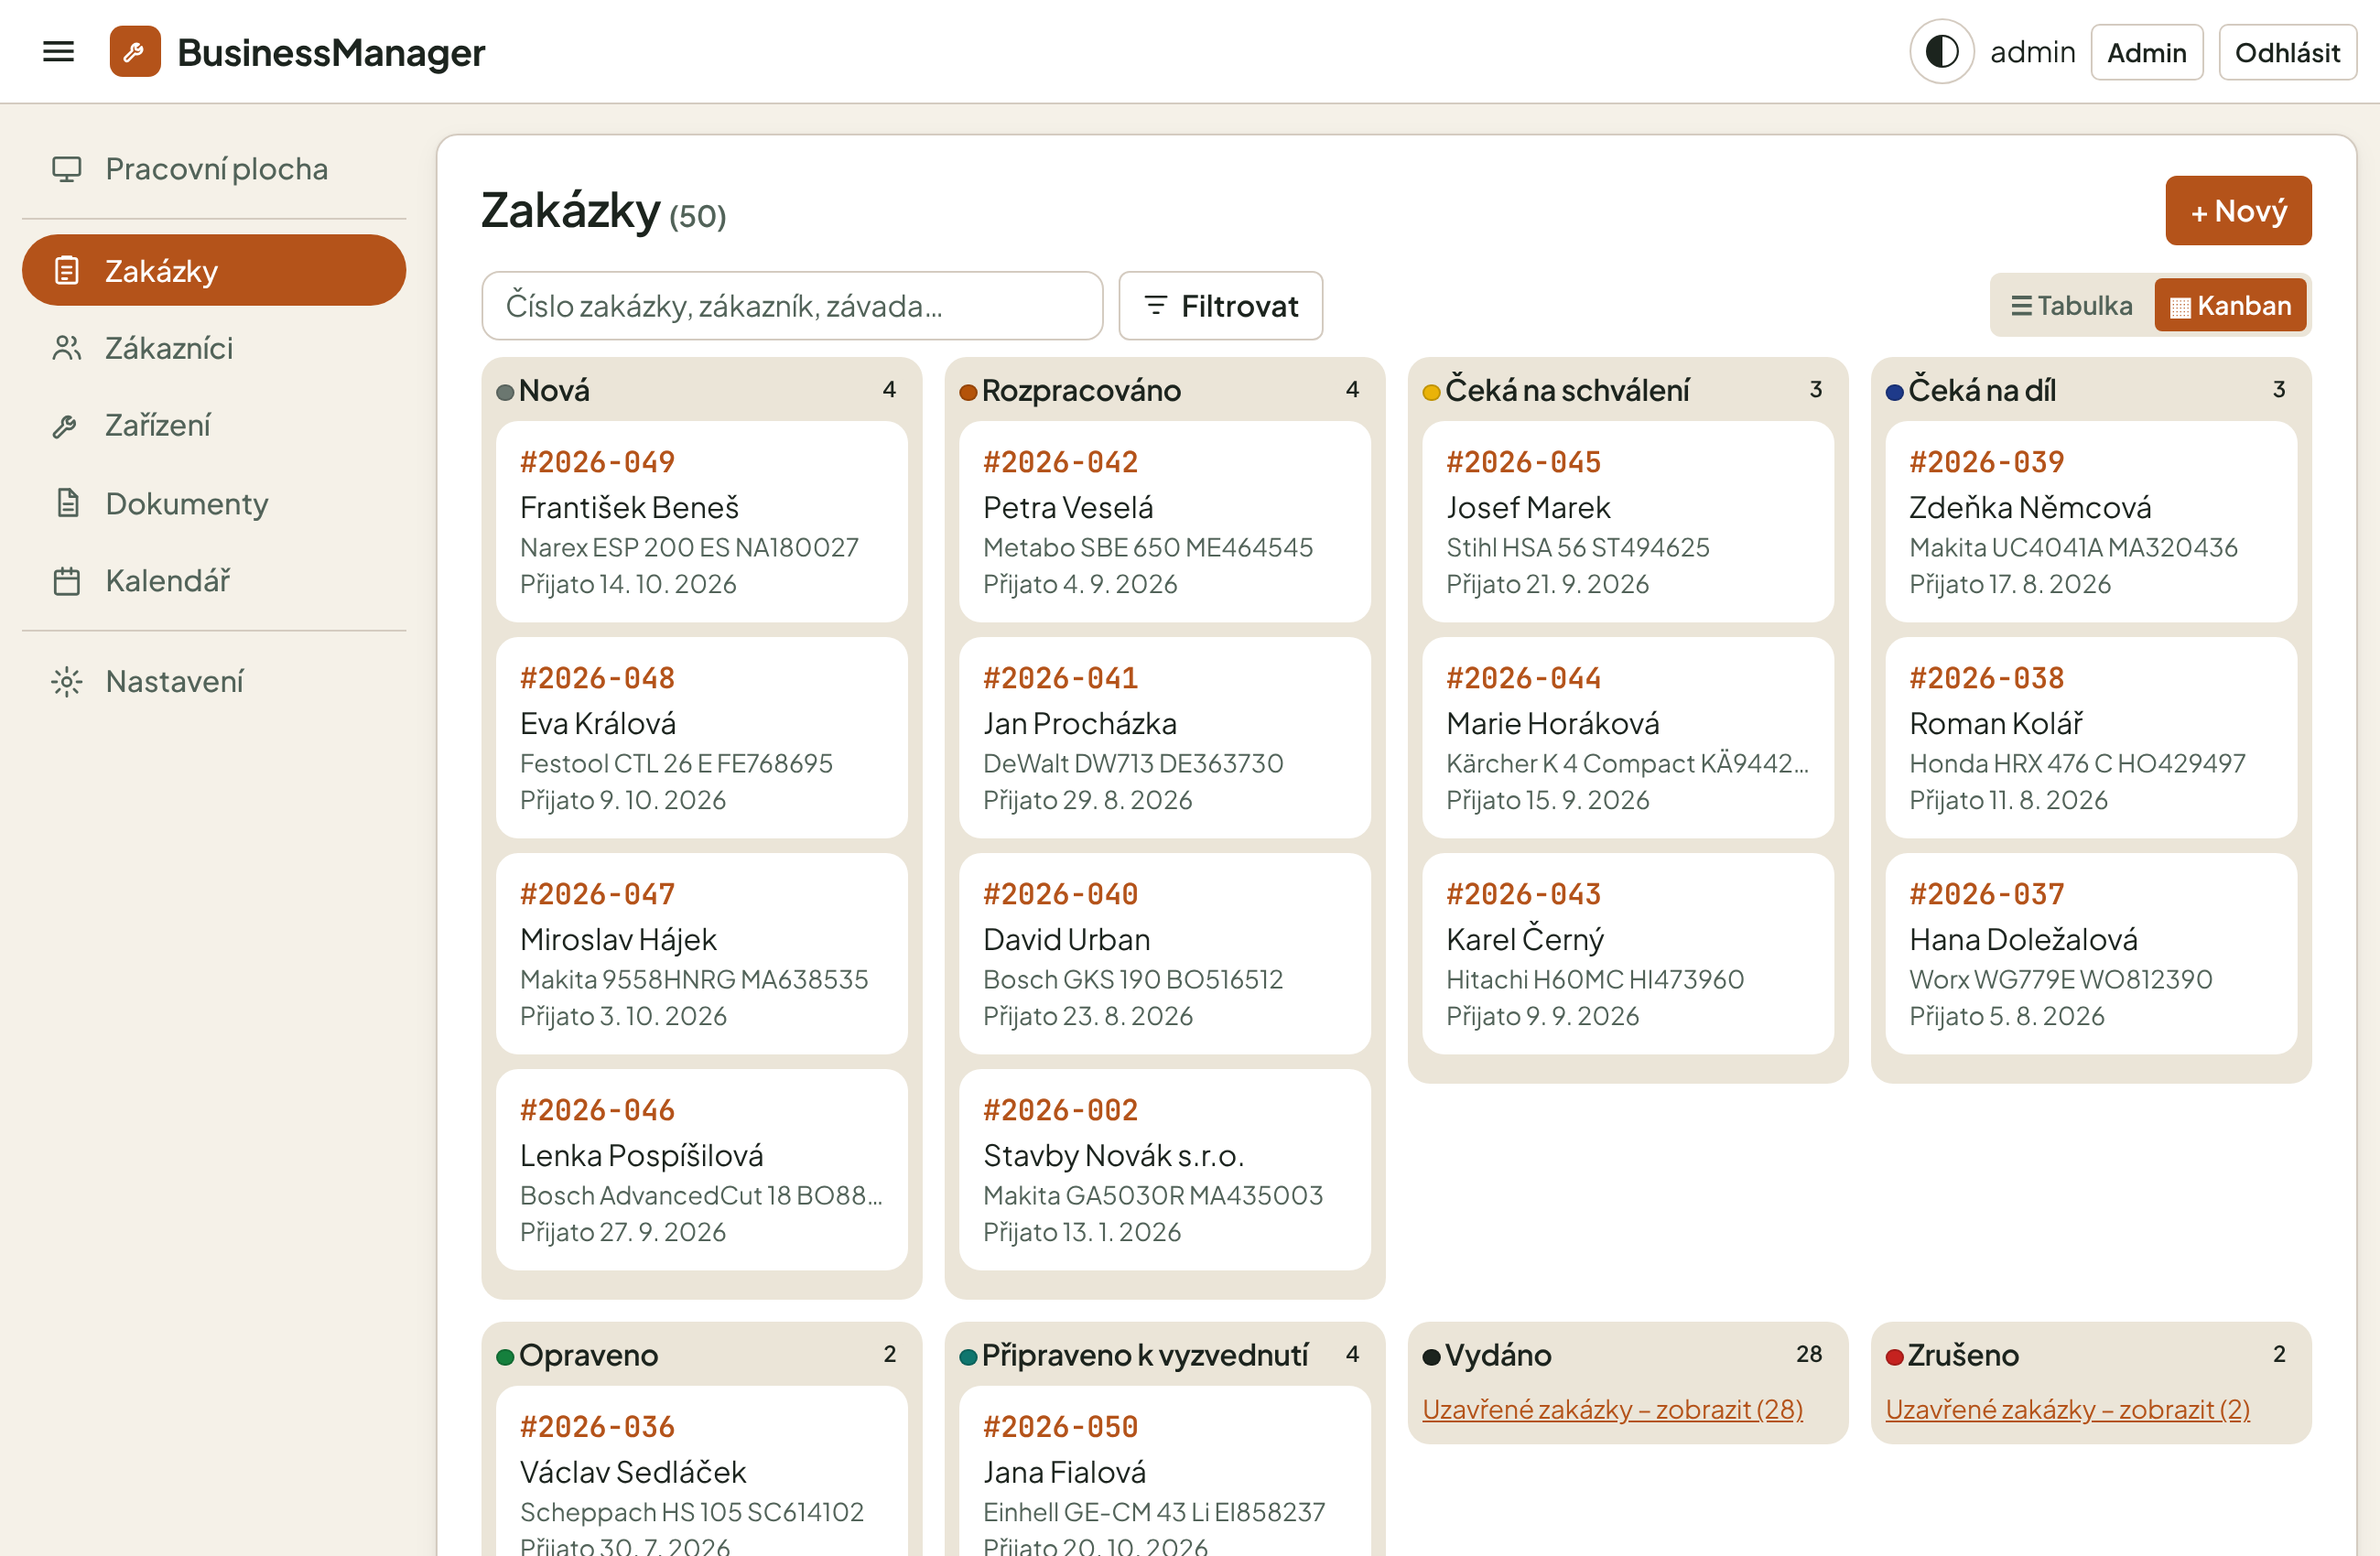
\includegraphics[width=\linewidth]{obrazky/navrh/bm-zakazky-kanban.png}
\caption{Kanbanové zobrazení zakázek v~aplikaci, sloupce odpovídají stavům zakázky, inspirováno Odoo (zdroj: vlastní)}\label{obr:bm-kanban}
\end{figure}

\subsection{Úpravy rozhraní podle doporučení}\label{sec:ui-upravy}

Při porovnání se zásadami vzniklo několik úprav a~všechny byly provedeny:
\begin{itemize}
\item Nastavení (údaje o~firmě, DPH, uživatelé, číselníky, šablony dokumentů, zálohování) bylo skryto a~zamčeno pro běžné zaměstnance. Později se rozdělení rozšířilo na role (Zaměstnanec, Technik, Administrativa, Administrátor): každý uživatel vidí jen tlačítka a~části aplikace, na které má oprávnění \cite{Nielsen-progressive}, \cite[s.~2331]{Sajedi2011}.
\item Styly Bootstrap a~knihovna htmx jsou přibaleny přímo do aplikace. Dříve se načítaly z~internetu a~bez připojení se aplikace zobrazila bez stylů, takže uživatel nevěděl, co se děje \cite{Nielsen-heuristiky}.
\item Při prvním spuštění provede aplikaci průvodce, který založí účet administrátora a~základní údaje o~firmě. Povinný je jen název organizace \cite{Nielsen-heuristiky}.
\item Na stránce zakázky bylo dříve osm stejně vypadajících tlačítek v~jedné řadě. Nyní zůstávají vpravo nahoře jen akce s~dokumenty (zakázkový list, nabídka, faktura, objednávka) a~tlačítka pro úpravu zakázky a~přidání práce, materiálu, fotografií a~příloh jsou v~záložkách, kterých se týkají. Plnou barvou je zvýrazněn jen doporučený další krok podle stavu zakázky, například zakázkový list u~nově přijaté zakázky, přidání práce u~rozpracované zakázky a~vytvoření nabídky a~poté faktury u~opravené zakázky. Je-li doporučeným krokem přidání práce, otevře se rovnou záložka Práce. Uživatel tak hned vidí, co má udělat dál \cite{Kaplan2021}, \cite{Shneiderman-pravidla}.
\item Na stránce zakázky byl dříve vpravo pevný panel prohlížeče dokumentů s~vlastní lištou tlačítek, který zabíral polovinu obrazovky i~tehdy, když uživatel žádný soubor neprohlížel. Nyní mají záložky celou šířku a~vejdou se do jedné řady. Fotografie, přílohy i~doklady se otevírají v~okně přes téměř celou obrazovku, ve kterém zůstalo jen stažení, tisk a~zavření, a~obrázek se přibližuje kolečkem myši. V~okně lze také porovnat dva soubory vedle sebe \cite{Nielsen-heuristiky}, \cite[s.~2332]{Sajedi2011}.
\item Údaje zařízení a~zákazníka se dříve upravovaly na samostatné stránce. Nyní tlačítko \enquote{Upravit} změní údaje přímo v~detailu na políčka a~tlačítka na \enquote{Uložit} a~\enquote{Zrušit}. Vedle údajů zařízení lze zobrazit fotografii nebo dokument z~jeho zakázek, například štítek s~typem a~sériovým číslem, takže je uživatel při přepisování nemusí držet v~paměti \cite{Shneiderman-pravidla}, \cite{Nielsen-heuristiky}.
\item Potvrzení nevratných akcí (například smazání) dříve zobrazoval systémový dialog prohlížeče s~adresou serveru. Nyní se zobrazí okno ve vzhledu aplikace se srozumitelnou otázkou a~tlačítkem, které říká, co se stane \cite{Shneiderman-pravidla}, \cite[s.~2331--2332]{Sajedi2011}.
\item Chybně zadaný e-mail nebo telefon dříve hlásila anglická bublina prohlížeče bez vysvětlení. Nyní formulář kontroluje server a~chybu ukáže česky u~políčka i~s~příkladem správného zápisu. Pole pro výběr souborů jsou také v~češtině \cite{Nielsen-heuristiky}.
\item Formuláře nové zakázky, nabídky a~faktury mají pod poli krátkou nápovědu, například že cena se zadává bez DPH a~DPH se dopočítá nebo že položky nabídky se převezmou ze zakázky \cite[s.~2330]{Sajedi2011}.
\end{itemize}

\endgroup

% ============================================================
% Praktická část, bod 3: Implementace systému pro evidenci zakázek
% ============================================================
\chapter{Implementace systému pro evidenci zakázek}\label{kap:funkce}

Tato kapitola popisuje, jak aplikace realizuje evidenci zakázek podle workflow z~oddílu~\ref{sec:workflow}: od přijetí zařízení přes zápis provedených prací a~materiálu až po vydání zařízení. Tvorbě nabídek a~faktur z~uložených dat se podrobně věnuje kapitola~\ref{kap:dokumenty}.

% delší názvy souborů a identifikátorů v textu se lépe zalomí
\begingroup\sloppy
% ============================================================
% Přehled funkcí (zkrácená verze; všechny funkce včetně toho, co se děje
% na pozadí, popisuje dokumentace aplikace: docs/02-funkce.md v repozitáři)
% ============================================================
\section{Přehled funkcí aplikace}\label{sec:funkce-aplikace}

Tento oddíl popisuje funkce, které plní požadavky z~kapitoly~\ref{kap:analyza-workflow}, tedy průběh zakázky od přijetí zařízení po vystavení dokladu. Přehled všech funkcí a~míst v~aplikaci, kde je uživatel najde, je v~tabulce~\ref{tab:funkce}. Podrobný popis každé funkce (k~čemu slouží, jak ji uživatel používá, co se děje na pozadí a~se kterými tabulkami pracuje) je součástí dokumentace aplikace\footnote{\url{https://github.com/MajkyyQ/BusinessManager/blob/main/docs/02-funkce.md}}.

\begin{longtable}{p{0.30\textwidth}p{0.60\textwidth}}
\caption{Přehled funkcí aplikace}\label{tab:funkce}\\
\hline \textbf{Funkce} & \textbf{Kde v aplikaci} \\ \hline\endfirsthead
\hline \textbf{Funkce} & \textbf{Kde v aplikaci} \\ \hline\endhead
Přijetí zakázky & Zakázky $\rightarrow$ Nová zakázka \\
Řízení stavu zakázky & detail zakázky, seznam zakázek (zobrazení kanban) \\
Evidence zákazníků a zařízení & Zákazníci, Zařízení (včetně historie oprav) \\
Fotografie a přílohy & detail zakázky \\
Práce a materiál & detail zakázky, Nastavení $\rightarrow$ Katalogy \\
Cenová nabídka, faktura a platby & detail zakázky, Dokumenty \\
Přijaté objednávky & detail zakázky, Dokumenty \\
Zakázkový list a výsledné dokumenty & detail zakázky, náhled dokumentu \\
Export faktury do ISDOC & náhled a detail faktury \\
Přijaté faktury & Dokumenty $\rightarrow$ Přijatá faktura z~ISDOC \\
Šablony dokumentů a číslování dokladů & Nastavení $\rightarrow$ Dokumenty \\
Pracovní plocha & úvodní stránka, detail zakázky \\
Kalendář & Kalendář \\
Vyhledávání & všechny formuláře a seznamy \\
Správa záznamů, zaměstnanci a oprávnění & Nastavení, administrace \\
Průvodce prvním spuštěním & po instalaci \\
Zálohování & Nastavení $\rightarrow$ Systém, skript \path{zaloha.bat} \\
První nastavení aplikace & Nastavení $\rightarrow$ První nastavení aplikace, pracovní plocha \\
Tmavý režim & přepínač v~horní liště \\
Historie změn & záložka Historie změn, Nastavení \\
\hline
\end{longtable}

\subsection{Přijetí zakázky}

Formulář \enquote{Nová zakázka} odpovídá dřívějšímu papírovému zakázkovému listu, a~proto jsou všechny údaje na jedné obrazovce v~pořadí, v~jakém je pracovník od zákazníka zjišťuje. Pracovník vyhledá zákazníka zadáním části jména, firmy, telefonu nebo IČO, a~pokud neexistuje, založí ho v~dialogovém okně bez opuštění formuláře. Stejně vybere nebo založí zařízení (nabízí se jen zařízení vybraného zákazníka) a~kontaktní osobu, zapíše popis závady a~nahraje fotografie. Po uložení aplikace v~jedné databázové transakci vytvoří zakázku se stavem \enquote{Nová}, přidělí jí číslo podle číselné řady, uloží navázané záznamy, zapíše událost do kalendáře a~záznam do historie změn.

\subsection{Řízení stavu zakázky}

Stav zakázky ukazuje, v~jaké fázi se oprava nachází, a~umožňuje rychle zjistit, která zařízení jsou ve firmě a~co je připraveno k~vyzvednutí. V~detailu zakázky se zobrazují jen tlačítka akcí, které jsou v~aktuálním stavu dovoleny (obrázek~\ref{fig:stavy}). Povolené přechody jsou v~kódu popsány dvěma slovníky (stav $\rightarrow$ povolené akce, akce $\rightarrow$ cílový stav) a~pohled akci před provedením ověří. Při vydání zařízení se uloží datum vydání a~kdo zařízení vydal. Ruční změnu stavu mimo pracovní postup smí jen administrátor nebo zaměstnanec s~oprávněním. Sám se stav mění jen u~nové zakázky: přidáním první práce přejde do stavu \enquote{Rozpracováno} a~vytvořením nabídky do stavu \enquote{Čeká na schválení}; obě změny se zapíší do historie. Každý stav má barvu, kterou si firma zvolí v~nastavení, a~vedle barvy je vždy uveden i~název stavu.

\begin{figure}[htbp]
\centering
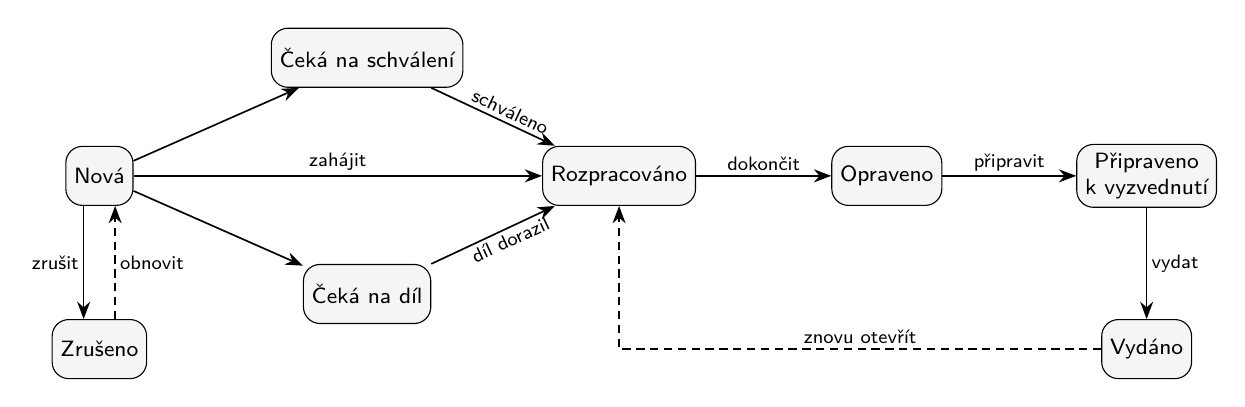
\begin{tikzpicture}[font=\footnotesize\sffamily,
    st/.style={draw, rounded corners=6pt, fill=gray!8, minimum height=0.75cm, inner sep=3pt, align=center},
    akce/.style={font=\scriptsize\sffamily, inner sep=1.5pt}]
  \node[st] (nova) at (0,0) {Nová};
  \node[st] (schv) at (3.4,1.5) {Čeká na schválení};
  \node[st] (dil) at (3.4,-1.5) {Čeká na díl};
  \node[st] (roz) at (6.6,0) {Rozpracováno};
  \node[st] (opr) at (10.0,0) {Opraveno};
  \node[st] (prip) at (13.3,0) {Připraveno\\k vyzvednutí};
  \node[st] (vyd) at (13.3,-2.2) {Vydáno};
  \node[st] (zrus) at (0,-2.2) {Zrušeno};
  \draw[bm sipka] (nova) -- node[akce, above] {zahájit} (roz);
  \draw[bm sipka] (nova) -- (schv);
  \draw[bm sipka] (nova) -- (dil);
  \draw[bm sipka] (schv) -- node[akce, above, sloped, pos=0.6] {schváleno} (roz);
  \draw[bm sipka] (dil) -- node[akce, below, sloped, pos=0.6] {díl dorazil} (roz);
  \draw[bm sipka] (roz) -- node[akce, above] {dokončit} (opr);
  \draw[bm sipka] (opr) -- node[akce, above] {připravit} (prip);
  \draw[bm sipka] (prip) -- node[akce, right] {vydat} (vyd);
  \draw[bm sipka] ([xshift=-2mm]nova.south) -- node[akce, left] {zrušit} ([xshift=-2mm]zrus.north);
  \draw[bm sipka, densely dashed] ([xshift=2mm]zrus.north) -- node[akce, right] {obnovit} ([xshift=2mm]nova.south);
  \draw[bm sipka, densely dashed] (vyd.west) -- node[akce, above] {znovu otevřít} (vyd.west -| roz.south) -- (roz.south);
\end{tikzpicture}
\caption{Hlavní přechody mezi stavy zakázky (zrušit lze i rozpracovanou zakázku a z rozpracované zakázky lze přejít zpět do čekání)}\label{fig:stavy}
\end{figure}

\subsection{Práce a materiál}

Evidence provedených prací a~použitého materiálu je podkladem pro ocenění zakázky a~pro položky dokladů. U~práce uživatel vybere typ úkonu z~katalogu, zadá cenu, sazbu DPH a~pracovníky. Materiál vyhledá v~katalogu a~zadá množství; aplikace sama doplní poslední známou cenu a~při uložení ji k~zakázce \enquote{zamrazí}, takže změna ceníku neovlivní starší zakázky. Tlačítkem \enquote{+ Přidat} lze do jednoho formuláře zapsat více prací nebo položek materiálu a~uložit je najednou. Poznámka k~práci je interní a~do zakázkového listu ani do položek dokladu se nepropisuje.

\subsection{Cenová nabídka, faktura a platby}

Nabídka i~faktura se vytvoří z~pracovní plochy zakázky. Formulář ukáže náhled položek, které budou převzaty, včetně součtů. Každá práce se stane položkou s~množstvím 1, každý materiál položkou s~množstvím, jednotkou a~cenou; chybějící sazbu DPH doplní výchozí sazba firmy. Položky vznikají jen ze zakázky, ručně se do vystaveného dokladu nepřidávají. Doklad dostane číslo podle číselné řady, kterou si firma nastaví podle vzoru (například \texttt{Fa0001} nebo \texttt{001-04-11/2026}), a~uloží si kopii údajů zákazníka. Nabídka přebírá pořadové číslo zakázky, další nabídka ke stejné zakázce dostane příponu (například \texttt{2026-048-2}). Po vytvoření nabídky aplikace nabídne pokračovat do zakázky nebo rovnou na fakturu. Spolu s~fakturou se založí platba ve stavu \enquote{Čeká na zaplacení}, kterou uživatel po úhradě jedním tlačítkem označí jako zaplacenou; obě události se zapíší do kalendáře.

Zákazník může zaplatit i~přímo při vyzvednutí zařízení bez faktury, typicky jen poplatek za diagnostiku, když se zařízení neopravuje. Tlačítko \enquote{Vydat zákazníkovi} proto otevře okno se dvěma volbami (obrázek~\ref{obr:bm-platba-na-miste}). Při volbě \enquote{Zaplaceno na místě bez faktury} uživatel potvrdí částku (předvyplní se součet práce a~materiálu s~DPH), zvolí způsob platby (hotově, QR kódem nebo kartou) a~může doplnit poznámku. Aplikace pak v~jedné databázové transakci založí platbu ve stavu \enquote{Zaplaceno} navázanou jen na zakázku a~zakázku vydá. Platba se zapíše do historie zakázky i~do kalendáře a~na pracovní ploše zakázky se zobrazí u~stavu. Volba \enquote{Bez platby na místě} slouží pro placení fakturou, záruční opravu nebo opravu zdarma. U~vydané zakázky bez faktury lze platbu zapsat i~dodatečně.

\begin{figure}[H]
\centering
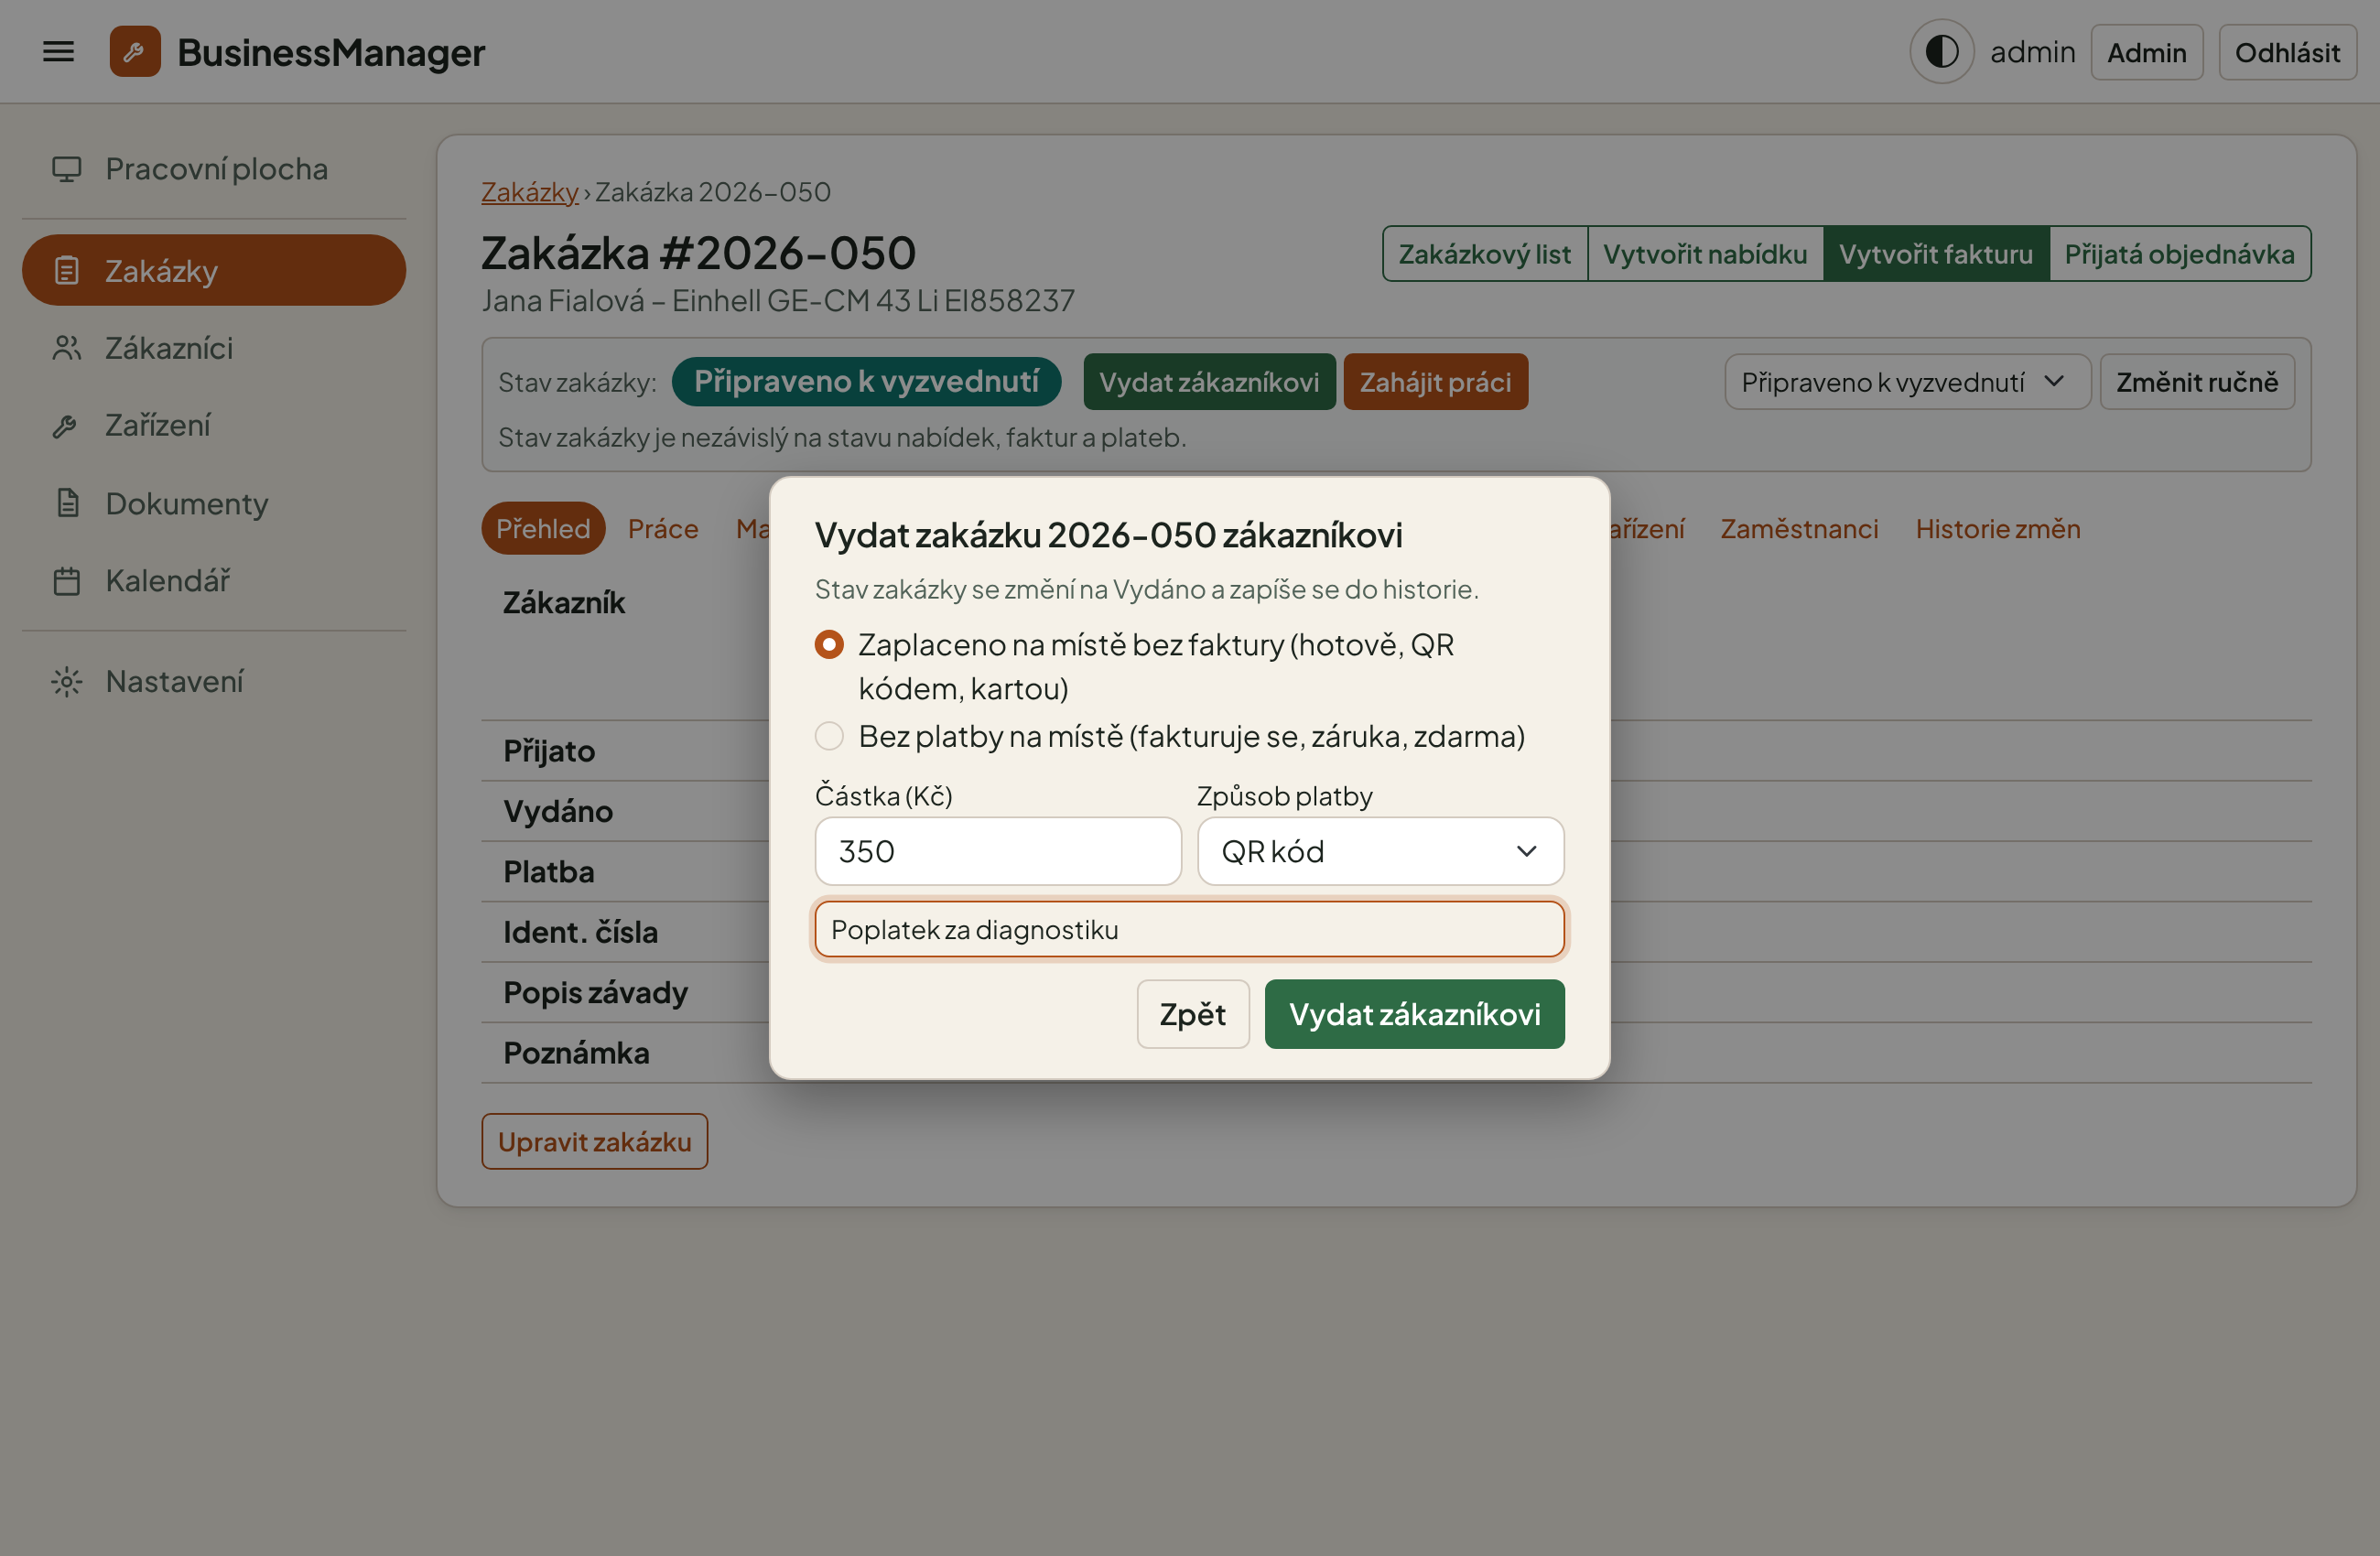
\includegraphics[width=\linewidth]{obrazky/navrh/bm-vydat-zaplaceno-na-miste.png}
\caption{Vydání zakázky se zápisem platby na místě bez faktury (zdroj: vlastní)}\label{obr:bm-platba-na-miste}
\end{figure}

Jak se data zakázky převedou na doklad a~dále na dokument, popisuje oddíl~\ref{sec:tok-dat}.

\subsection{Výsledné dokumenty}

Zakázkový list, nabídku i~fakturu lze zobrazit v~náhledu, vytisknout nebo stáhnout jako PDF s~názvem podle firemních zvyklostí. Volba \enquote{Změnit šablonu} zobrazí miniatury všech šablon daného typu a~kliknutím se dokument zobrazí v~jiné šabloně. Fakturu lze stáhnout i~jako elektronickou fakturu ISDOC. Systém šablon popisuje oddíl~\ref{sec:sablony}.

\subsection{Přijaté faktury a kalendář}\label{sec:prijate-faktury}

Faktury od dodavatelů uživatel nahraje jako soubor ISDOC. Aplikace z~něj přečte údaje faktury a~dodavatele, dodavatele dohledá v~evidenci nebo založí, upozorní na duplicitní fakturu a~uloží záznam s~původním souborem. Do kalendáře se zapíše doručení, splatnost a~po úhradě i~zaplacení. Fakturu, která přišla jen na papíře, lze zadat ručně.

Kalendář sdružuje automatické události (přijetí a~vydání zakázek, vystavení a~zaplacení faktur, splatnost přijatých faktur) s~ručně zadanými termíny. Lze ho zobrazit po měsících, týdnech nebo dnech a~filtrovat podle typu události a~zaměstnance. V~měsíčním zobrazení se u~dne ukážou nejvýše tři události, kliknutím na den se otevře okno se všemi událostmi dne. Vlastní událost lze rychle přidat tlačítkem \enquote{+} přímo u~dne.

\endgroup

% ============================================================
% Praktická část, bod 4: Implementace automatizované tvorby nabídek
% a faktur z uložených dat
% ============================================================
\chapter{Implementace automatizované tvorby nabídek a~faktur z~uložených dat}\label{kap:dokumenty}

Nabídka a~faktura v~aplikaci vznikají z~údajů, které jsou už uložené u~zakázky, stejně jako v~integrovaných systémech popsaných v~oddílu~\ref{sec:zakazka-doklady}. Tato kapitola popisuje systém šablon, podle kterých se doklady tisknou, a~tok dat od zadání zakázky po hotový dokument.

% delší názvy souborů a identifikátorů v textu se lépe zalomí
\begingroup\sloppy
% ============================================================
% Systém šablon dokumentů (zkrácená verze; úplný popis včetně editoru
% šablon, formátu mapování a importu ISDOC je v dokumentaci aplikace:
% docs/08-sablony-dokumentu.md v repozitáři)
% ============================================================
\section{Systém šablon dokumentů}\label{sec:sablony}

Systém šablon určuje, jak se data uložená v~databázi promění ve výsledný dokument: zakázkový list, cenovou nabídku nebo fakturu. Hlavním požadavkem firmy bylo zachovat vzhled dosavadních Excelových formulářů a~umožnit jejich pozdější úpravy bez zásahu do zdrojového kódu. Systém proto stojí na třech principech:

\begin{enumerate}
\item \textbf{Oddělení dat a vzhledu.} Šablona obsahuje pouze vzhled dokumentu a~informaci o~tom, kam se vkládají jednotlivé údaje. Data dokumentu se vždy sestavují z~databáze. Šablona nikdy data nemění a~stejná data lze zobrazit v~libovolné šabloně.
\item \textbf{Šablonou je běžný soubor aplikace Excel.} Firma může vzít svůj stávající formulář, vložit do něj značky a~nahrát ho do aplikace. Formátování, sloučené buňky, vzorce, obrázky i~tvary zůstanou zachovány.
\item \textbf{Rozšiřitelnost.} Typy dokumentů a~formáty šablon jsou v~kódu samostatné třídy, takže nový typ dokumentu nebo nový formát lze přidat bez změny ostatních částí.
\end{enumerate}

Průběh od nahrání šablony po vytvoření PDF ukazuje obrázek~\ref{fig:sablony}. Horní řada znázorňuje přípravu šablony, která proběhne jednou při jejím nahrání nebo úpravě, dolní řada tvorbu dokumentu při každém zobrazení. Podrobný popis jednotlivých kroků, formátu uloženého mapování a~webového editoru šablon je součástí dokumentace aplikace\footnote{\url{https://github.com/MajkyyQ/BusinessManager/blob/main/docs/08-sablony-dokumentu.md}}.

\begin{figure}[H]
\centering
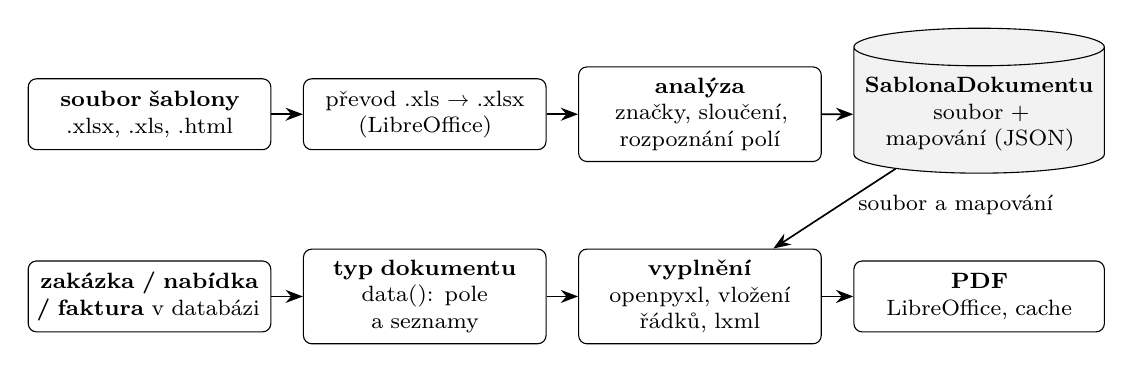
\begin{tikzpicture}[node distance=6mm and 4mm, font=\footnotesize]
  \node[bm blok, text width=2.8cm] (soubor) {\textbf{soubor šablony}\\\texttt{.xlsx}, \texttt{.xls}, \texttt{.html}};
  \node[bm blok, right=of soubor, text width=2.8cm] (prevod) {převod \texttt{.xls} $\rightarrow$ \texttt{.xlsx}\\(LibreOffice)};
  \node[bm blok, right=of prevod, text width=2.8cm] (analyza) {\textbf{analýza}\\značky, sloučení, rozpoznání polí};
  \node[bm uloziste, right=of analyza, text width=2.9cm, font=\footnotesize] (sablona) {\textbf{Sablona\-Dokumentu}\\soubor + mapování (JSON)};
  \node[bm blok, below=14mm of soubor, text width=2.8cm] (objekt) {\textbf{zakázka / nabídka / faktura} v databázi};
  \node[bm blok, right=of objekt, text width=2.8cm] (data) {\textbf{typ dokumentu}\\\texttt{data()}: pole a~seznamy};
  \node[bm blok, right=of data, text width=2.8cm] (vypln) {\textbf{vyplnění}\\openpyxl, vložení řádků, lxml};
  \node[bm blok, right=of vypln, text width=2.9cm] (pdf) {\textbf{PDF}\\LibreOffice, cache};
  \draw[bm sipka] (soubor) -- (prevod);
  \draw[bm sipka] (prevod) -- (analyza);
  \draw[bm sipka] (analyza) -- (sablona);
  \draw[bm sipka] (objekt) -- (data);
  \draw[bm sipka] (data) -- (vypln);
  \draw[bm sipka] (vypln) -- (pdf);
  \draw[bm sipka] (sablona) -- node[pos=0.45, right=1mm, align=left] {soubor a~mapování} (vypln);
\end{tikzpicture}
\caption{Příprava šablony a tvorba dokumentu}\label{fig:sablony}
\end{figure}

\subsection{Typy dokumentů a data dokumentu}

Pro každý typ dokumentu (zakázkový list, nabídka, faktura) definuje modul \path{core/sablony/typy.py} katalog asi osmdesáti polí, která lze do šablony vložit. Pole mají klíč ve tvaru \texttt{skupina.nazev} (například \texttt{zakaznik.ico}), druh hodnoty (text, číslo, peníze, datum, obrázek), podle kterého se hodnota formátuje, a~synonyma, podle kterých je lze najít v~šabloně bez značek. Kromě jednoduchých polí existují tři seznamy opakujících se řádků: položky dokladu, materiál a~práce. Metoda \texttt{data()} typu dokumentu sestaví z~objektu v~databázi data, která mají vždy stejný tvar, nezávislý na typu dokumentu i~na formátu šablony (výpis~\ref{lst:data}).

\begin{lstlisting}[showstringspaces=false, columns=fullflexible, keepspaces=true, basicstyle=\footnotesize\ttfamily, caption={Tvar dat dokumentu (zkráceno)}, label={lst:data}]
{"pole": {"dokument.cislo": "001-27-10/2026",
          "dokument.datum_splatnosti": date(2026, 11, 10),
          "firma.nazev": "...", "zakaznik.ico": "12345678",
          "zakazka.cislo": "2026-048", "zarizeni.typ": "GSR 18V",
          "soucty.s_dph": Decimal("3633.75"), ...},
 "polozky":  [{"polozka.popis": "Diagnostika", "polozka.mnozstvi": Decimal("1"),
               "polozka.cena_bez_dph": Decimal("1500.00"), ...}, ...],
 "material": [{"material.nazev": "Ložisko 6204-2RS", ...}, ...],
 "prace":    [{"prace.popis": "Petr Svoboda: Diagnostika", ...}, ...]}
\end{lstlisting}

\subsection{Značky a rozpoznání šablony}

Místo pro údaj se v~šabloně označí \emph{značkou} ve tvaru \texttt{\{\{skupina.pole\}\}}, například \texttt{\{\{zakaznik.nazev\}\}}. Značka může tvořit celý obsah buňky, nebo být součástí textu, například \texttt{Faktura č. \{\{dokument.cislo\}\}}. Řádek se značkou některého seznamu (\texttt{\{\{polozka.\ldots\}\}}) je vzorovým řádkem tabulky, který se zopakuje pro každou položku. Při nahrání šablony ji aplikace analyzuje, značky uloží jako \emph{mapování} ve formátu JSON a~upozorní na neznámé značky, typicky překlepy. Pokud šablona značky neobsahuje, pokusí se aplikace najít místa pro údaje podle popisků formuláře (například \enquote{IČO:} nebo hlavičky tabulky \enquote{Popis}, \enquote{Množství}, \enquote{Celkem}). Výsledek je jen návrh, který uživatel může opravit ve webovém editoru šablon. Ten zobrazí list šablony jako mřížku buněk a~pole do ní uživatel přetahuje myší, takže k~úpravě šablony nepotřebuje Excel.

\subsection{Vyplnění šablony}

Šablonu vyplňuje funkce \texttt{vypln} vždy v~kopii sešitu, původní soubor se nemění. Je-li v~buňce jen značka, zapíše se skutečná hodnota odpovídajícího typu (číslo jako číslo, datum jako datum), aby s~ní mohly počítat vzorce šablony; pokud buňka nemá vlastní formát, nastaví se český formát. Značka uvnitř textu se nahradí naformátovaným textem. Logo firmy se vloží jako obrázek zmenšený do vyhrazené oblasti. Firemní formuláře intenzivně využívají sloučené buňky, proto aplikace nepracuje s~jednotlivými buňkami, ale s~oblastmi.

Nejsložitější částí je \textbf{rozšíření tabulky položek}. Faktura může mít jednu položku i~dvacet, šablona ale obsahuje jen jeden vzorový řádek a~pod tabulkou často pokračuje dalším obsahem (součty, platební údaje, podpisy). Aplikace nejprve využije předkreslené prázdné řádky tabulky. Pokud nestačí, vloží chybějící řádky a~přitom posune sloučené oblasti, výšky řádků, obrázky a~tiskovou oblast, zkopíruje styly vzorového řádku a~upraví odkazy ve vzorcích, takže například \texttt{=SUM(H21:H21)} se změní na \texttt{=SUM(H21:H25)}. Tabulky se vyplňují odspodu nahoru, aby vložení řádků do spodní tabulky neposunulo tabulky nad ní. Grafické tvary (rámečky, čáry, textová pole), které knihovna openpyxl při uložení ztrácí, přenese aplikace pomocí knihovny lxml z~původního souboru a~posune je o~vložené řádky.

Kromě Excelových šablon podporuje aplikace i~šablony HTML v~šablonovacím jazyce Django. Jejich náhled se zobrazí i~bez LibreOffice, a~proto slouží jako záložní řešení.

\subsection{Export do PDF}

Vyplněný sešit převede do PDF LibreOffice spuštěný bez grafického rozhraní s~vlastním profilem s~českým národním prostředím, aby se čísla a~data formátovala česky. LibreOffice při převodu přepočítá vzorce a~respektuje tiskovou oblast, sloučené buňky, ohraničení, obrázky i~tvary. Převody probíhají postupně, protože LibreOffice nesmí běžet se stejným profilem dvakrát současně. Hotové PDF se uloží do vyrovnávací paměti pod klíčem, který je hašem verze šablony, mapování a~kompletních dat dokumentu. Opakované zobrazení stejného dokumentu je proto okamžité a~jakákoli změna dat nebo šablony vytvoří nové PDF.

\subsection{Export do formátu ISDOC}\label{sec:isdoc}

ISDOC je český standard pro výměnu elektronických faktur ve formátu XML, který podporuje většina tuzemských účetních programů. Faktura ISDOC obsahuje strukturovaná data (dodavatel, odběratel, data, položky, sazby a~částky DPH, platební údaje), takže ji příjemce načte do účetnictví bez přepisování. ISDOC nepopisuje vzhled, ale jen data, proto nevzniká ze šablony, ale přímo z~výsledku metody \texttt{data()} typu dokumentu Faktura. Tištěná faktura a~faktura ISDOC tak vždy obsahují stejné položky a~částky. Přiřazení údajů k~prvkům formátu ukazuje tabulka~\ref{tab:isdoc}.

\begin{longtable}{p{0.40\textwidth}p{0.52\textwidth}}
\caption{Přiřazení údajů faktury k~prvkům formátu ISDOC}\label{tab:isdoc}\\
\hline \textbf{Prvek ISDOC} & \textbf{Zdroj v aplikaci} \\ \hline\endfirsthead
\hline \textbf{Prvek ISDOC} & \textbf{Zdroj v aplikaci} \\ \hline\endhead
\texttt{ID}, \texttt{UUID} & \texttt{dokument.cislo}; UUID odvozené z~identifikace faktury \\
\texttt{IssueDate}, \texttt{TaxPointDate} & \texttt{dokument.datum\_vystaveni}, \texttt{dokument.duzp} \\
\texttt{AccountingSupplierParty} & údaje firmy z~nastavení (\texttt{firma.*}) \\
\texttt{AccountingCustomerParty} & údaje zákazníka (\texttt{zakaznik.*}) \\
\texttt{InvoiceLines} & seznam \texttt{polozky} \\
\texttt{TaxTotal} & rekapitulace DPH vypočtená z~položek podle sazeb \\
\texttt{LegalMonetaryTotal} & součty bez DPH, s~DPH a~částka k~úhradě \\
\texttt{PaymentMeans} & číslo účtu firmy, datum splatnosti, variabilní symbol \\
\hline
\end{longtable}

Při převodu aplikace rozdělí adresu uloženou jako jeden text na ulici, číslo, PSČ a~město, rozdělí číslo účtu na účet a~kód banky, spočítá rekapitulaci DPH zvlášť pro každou sazbu a~odvodí stálý identifikátor UUID z~identifikace faktury. Hotový dokument se před odesláním ověří proti oficiálnímu schématu XSD formátu ISDOC~6.0.2, takže aplikace nikdy nevydá neplatnou fakturu. Správnost převodu ověřují automatické testy (oddíl~\ref{sec:testovani-automaticke}).

Stejný modul čte i~faktury ISDOC od dodavatelů (oddíl~\ref{sec:prijate-faktury}). Načítá je s~vypnutým rozbalováním entit a~přístupem k~síti, aby nahraný soubor nemohl číst jiné soubory serveru (ochrana proti útoku XXE), a~zvládá formáty ISDOC~5 i~6 i~zabalený formát ISDOCX.\label{sec:isdoc-import}

% ============================================================
% Tok dat aplikací (zkrácená verze; jednotlivé kroky podrobně popisuje
% dokumentace aplikace: docs/06-tok-dat.md v repozitáři)
% ============================================================
\section{Tok dat aplikací}\label{sec:tok-dat}

Tento oddíl propojuje popsané součásti a~sleduje, jak data procházejí systémem od zadání zakázky po výsledný dokument (obrázek~\ref{fig:tok-dat}). Údaje zakázky se zadávají formulářem a~ukládají v~jedné transakci, během opravy se k~zakázce přidávají práce, materiál a~další záznamy. Při vytvoření nabídky nebo faktury se z~prací a~materiálu stanou položky dokladu. Při zobrazení dokumentu typ dokumentu sestaví data ve standardizovaném tvaru (výpis~\ref{lst:data}), doplní je o~údaje firmy a~odvozené hodnoty, vloží je do zvolené šablony a~LibreOffice výsledek převede na PDF. Elektronická faktura ISDOC vzniká ze stejných dat, jen místo do šablony se data převedou rovnou do XML, takže PDF a~ISDOC si nemohou odporovat. Podrobný popis jednotlivých kroků je součástí dokumentace aplikace\footnote{\url{https://github.com/MajkyyQ/BusinessManager/blob/main/docs/06-tok-dat.md}}.

\begin{figure}[htbp]
\centering
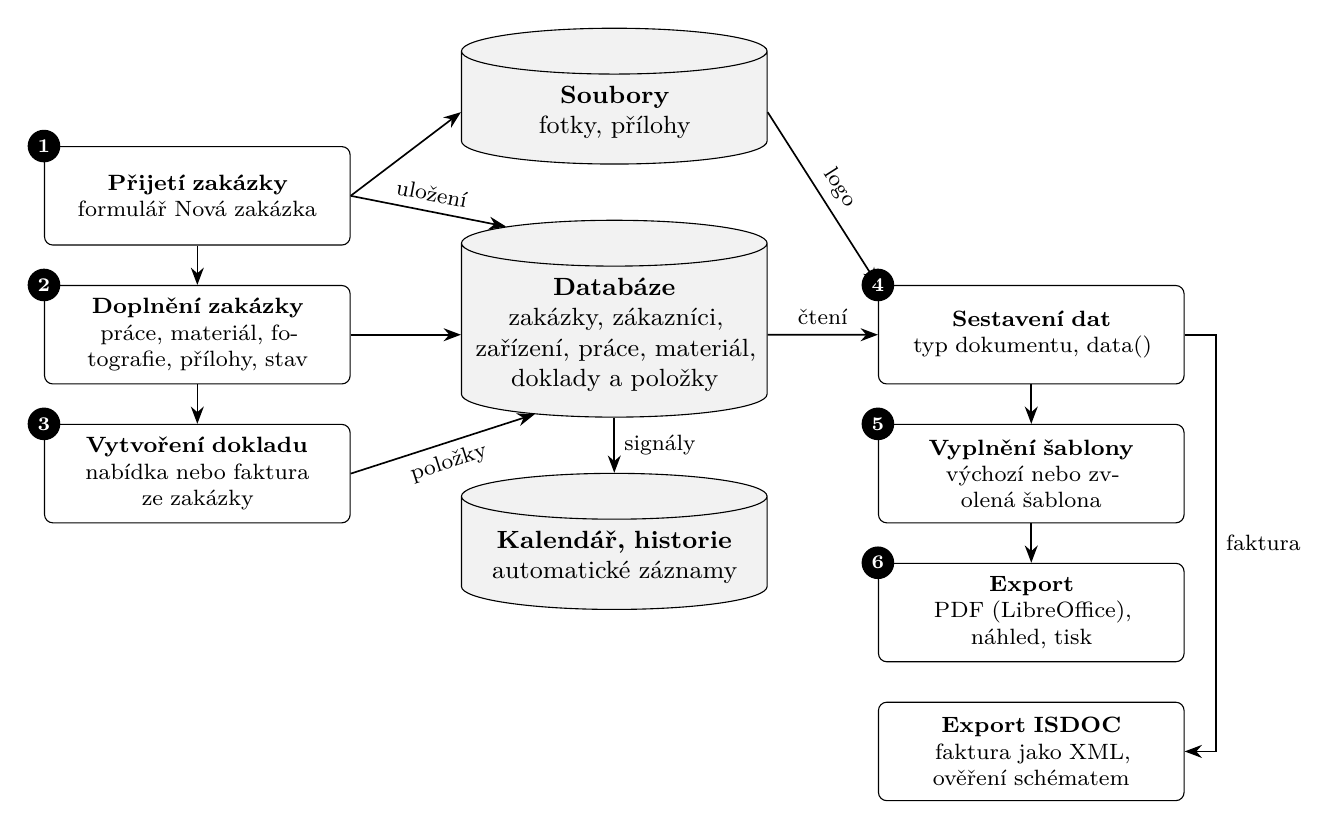
\begin{tikzpicture}[node distance=5mm and 5mm, font=\footnotesize,
    krok/.style={bm blok, text width=3.6cm, minimum height=1.25cm},
    cislo/.style={circle, draw, fill=black, text=white, font=\scriptsize\bfseries, inner sep=1pt, minimum size=4mm}]
  % levý sloupec – zadání dat
  \node[krok] (k1) {\textbf{Přijetí zakázky}\\formulář Nová zakázka};
  \node[krok, below=of k1] (k2) {\textbf{Doplnění zakázky}\\práce, materiál, fotografie, přílohy, stav};
  \node[krok, below=of k2] (k3) {\textbf{Vytvoření dokladu}\\nabídka nebo faktura\\ze zakázky};
  % prostřední sloupec – databáze
  \node[bm uloziste, right=14mm of k2, text width=3.6cm] (db) {\textbf{Databáze}\\zakázky, zákazníci, zařízení, práce, materiál, doklady a~položky};
  \node[bm uloziste, above=7mm of db, text width=3.6cm] (media) {\textbf{Soubory}\\fotky, přílohy};
  \node[bm uloziste, below=7mm of db, text width=3.6cm] (kal) {\textbf{Kalendář, historie}\\automatické záznamy};
  % pravý sloupec – dokument
  \node[krok, right=14mm of db] (k4) {\textbf{Sestavení dat}\\typ dokumentu, \texttt{data()}};
  \node[krok, below=of k4] (k5) {\textbf{Vyplnění šablony}\\výchozí nebo zvolená šablona};
  \node[krok, below=of k5] (k6) {\textbf{Export}\\PDF (LibreOffice),\\náhled, tisk};
  \node[krok, below=of k6] (k7) {\textbf{Export ISDOC}\\faktura jako XML,\\ověření schématem};
  % čísla kroků
  \foreach \n in {1,...,6} \node[cislo] at (k\n.north west) {\n};
  % šipky
  \draw[bm sipka] (k1) -- (k2);
  \draw[bm sipka] (k2) -- (k3);
  \draw[bm sipka] (k1.east) -- node[above, sloped] {uložení} (db.north west);
  \draw[bm sipka] (k2.east) -- (db.west);
  \draw[bm sipka] (k1.east) -- (media.west);
  \draw[bm sipka] (k3.east) -- node[below, sloped] {položky} (db.south west);
  \draw[bm sipka] (db) -- node[right] {signály} (kal);
  \draw[bm sipka] (db) -- node[above] {čtení} (k4);
  \draw[bm sipka] (k4) -- (k5);
  \draw[bm sipka] (k5) -- (k6);
  \draw[bm sipka] (k4.east) -- ++(4mm,0) |- node[right, pos=0.25] {faktura} (k7.east);
  \draw[bm sipka] (media.east) -- node[above, sloped] {logo} (k4.north west);
\end{tikzpicture}
\caption{Tok dat od zadání zakázky po výsledný dokument}\label{fig:tok-dat}
\end{figure}

Z~toku dat vyplývají tři vlastnosti, na kterých stojí návrh celé aplikace:

\begin{itemize}
\item \textbf{Jedno místo zadání.} Každý údaj (zákazník, zařízení, cena materiálu) se zadá jednou a~dále se na něj jen odkazuje. Všechny výstupy z~něj vznikají automaticky.
\item \textbf{Jasný okamžik zamrazení.} Zdrojová data zakázky se mohou měnit až do vytvoření dokladu. Doklad si uloží vlastní kopii položek a~údajů zákazníka, a~zůstává proto ve stavu, v~jakém byl vystaven. Zakázkový list vlastní kopii nemá a~vždy ukazuje aktuální stav zakázky.
\item \textbf{Dokument je pohled na data.} Výsledné dokumenty se neukládají, ale vždy se sestaví z~databáze a~šablony. Změna šablony změní vzhled všech dokumentů, nikoli jejich obsah, a~oprava dat se projeví ve všech dokumentech, které se z~nich znovu vytvoří.
\end{itemize}

\endgroup

% ============================================================
% Praktická část, bod 5: Testování, nasazení aplikace do provozu
% a vyhodnocení zpětné vazby od zaměstnanců
% Oddíly označené [DOPLNIT] dopíše autor.
% ============================================================
\chapter{Testování, nasazení aplikace do provozu a~vyhodnocení zpětné vazby od zaměstnanců}\label{kap:testovani}

\section{Přístup k~testování}\label{sec:testovani-pristup}

Sommerville rozlišuje dvě otázky, na které testování odpovídá. \emph{Verifikace} ověřuje, zda software splňuje stanovené funkční a~nefunkční požadavky. \emph{Validace} ověřuje, zda software dělá to, co zákazník skutečně očekává \cite[s.~228]{Sommerville2016}. Komerční software podle něj prochází třemi fázemi testování: \emph{vývojovým testováním} během vývoje, \emph{testováním vydání}, kdy se ověřuje celá verze před předáním uživatelům, a~\emph{uživatelským testováním} v~prostředí uživatele \cite[s.~231]{Sommerville2016}.

Vývojové testování se dále dělí na testování jednotek (jednotlivých funkcí a~tříd), testování komponent a~testování systému jako celku \cite[s.~232]{Sommerville2016}. Automatizované testy jsou zapsány jako program, který se spustí při každé změně. Jsou rychlejší než ruční testování, zejména u~\emph{regresního testování}, kdy se po změně znovu spustí všechny dřívější testy a~ověří se, že změna nic nerozbila \cite[s.~231]{Sommerville2016}. Automaticky však nelze otestovat, jak rozhraní vypadá, proto se automatické testy doplňují ručním testováním \cite[s.~231]{Sommerville2016}.

Aplikace byla testována ve všech třech fázích. Vývojové testování tvoří automatické testy a~ruční zkoušky v~prohlížeči, testováním vydání je ověření celé verze na čisté instalaci a~uživatelským testováním je pilotní provoz ve firmě (oddíl~\ref{sec:nasazeni}).

\section{Testovací prostředí}\label{sec:testovani-prostredi}

Aplikace byla testována na vývojovém počítači autora. % [DOPLNIT] ověřit a doplnit údaje
\begin{itemize}
\item počítač: Lenovo Legion~7, operační systém Windows~11 Home 24H2, procesor Intel Core i9 14900HX , paměť RAM 32GB,
\item Python~3.13 a~Django~5.2,
\item databáze SQLite (vývojová instalace) a~PostgreSQL (instalace v~Dockeru, která odpovídá provozu ve firmě),
\item webový prohlížeč Mozilla FireFox.
\end{itemize}

Aplikace se vyvíjí a~průběžně testuje nad databází SQLite. Ta je uložena v~jednom souboru a~nevyžaduje instalaci databázového serveru, takže vývoj a~spouštění testů jsou jednoduché a~rychlé. Ve firmě však aplikace poběží nad databází PostgreSQL v~Dockeru, která lépe zvládá souběžnou práci více uživatelů. Oba systémy se v~některých podrobnostech liší, například v~kontrole integritních omezení nebo v~porovnávání textu. Aplikace k~databázi přistupuje jen přes ORM frameworku Django (oddíl~\ref{sec:principy-orm}), takže stejný kód funguje nad oběma systémy. Aby se ověřilo, že se aplikace chová stejně i~v~reálném provozu, byly všechny automatické testy spuštěny nad SQLite i~nad PostgreSQL.

\section{Automatické testy}\label{sec:testovani-automaticke}

Automatické testy jsou napsány pomocí testovacího nástroje frameworku Django a~jsou uloženy v~souboru \path{core/tests.py}. Spouští se příkazem \texttt{python manage.py test core}. Každý test si vytvoří vlastní prázdnou databázi, takže výsledek nezávisí na datech uložených v~aplikaci. Testy pokrývají části aplikace, ve kterých by chyba měla největší následky: správnost dokladů, integritu dat, oprávnění a~bezpečnost. Přehled všech testů s~popisem toho, co ověřují, a~výsledky jejich spuštění nad databázemi SQLite a~PostgreSQL jsou v~dokumentaci aplikace\footnote{\url{https://github.com/MajkyyQ/BusinessManager/blob/main/docs/09-vyvoj-a-testovani.md}}.

\subsection{Testy bezpečnosti}

Zvláštní pozornost byla věnována útoku SQL injection, který popisuje oddíl~\ref{sec:principy-sql-injection}. Testy zkoušejí přihlášení s~devíti typickými útočnými řetězci ve jménu, v~hesle i~v~obou polích zároveň a~ověřují, že se žádný pokus nepřihlásí a~tabulka uživatelů zůstane beze změny. Dále ověřují, že útočné řetězce ve vyhledávání a~v~parametru řazení seznamu nevrátí cizí data ani nezpůsobí chybu. Podrobnosti jsou v~oddílu~\ref{sec:db-sql-injection}.

\subsection{Bezpečnostní audit}\label{sec:bezpecnostni-audit}

Před zveřejněním aplikace jako open source prošel zdrojový kód aplikace i~modulu Odesílání e-mailů bezpečnostním auditem. Audit postupoval podle metodiky \emph{security-audit}, která za chybu považuje jen porušení skutečné hranice důvěry. U~každého nálezu proto musí být jasné, kdo chybu může zneužít, co tím získá a~která kontrola v~aplikaci selhala. Obecná doporučení bez konkrétního dopadu se vedou zvlášť jako doporučení pro provoz.

Audit vycházel z~toho, pro jaký provoz je aplikace navržená. Aplikace je navržená pro malou firmu v~uzavřené firemní síti. Chrání data před uživateli bez oprávnění a~před lidmi v~síti bez účtu. Nechrání před tím, kdo má přístup přímo k~serverovému PC, protože to patří k~zabezpečení počítače, ne aplikace. Kdo má přístup k~serverovému počítači fyzicky nebo jako jeho správce, má přístup i~k~databázi a~souborům a~žádné zabezpečení uvnitř aplikace ho nezastaví. Útočník ve stejné síti ale k~databázi přístup nemá, protože se databáze do sítě nepublikuje, a~bez účtu uvidí jen přihlašovací stránku. Aplikace také není určená k~vystavení do internetu.

Audit dále vycházel z~rolí a~oprávnění aplikace a~z~toho, odkud do aplikace přicházejí data. Posuzovaly se tyto hranice důvěry:
\begin{itemize}
	\item nepřihlášený návštěvník ve firemní síti nesmí vidět žádnou stránku ani soubor kromě přihlášení a~průvodce prvním spuštěním,
	\item zaměstnanec se základní rolí nesmí vidět doklady bez oprávnění, měnit nastavení, mazat cizí záznamy ani získat vyšší oprávnění,
	\item technik a~administrativa nesmí překročit oprávnění své role,
	\item uživatel s~oprávněním Nastavení nesmí převzít účet hlavního administrátora,
	\item soubor od zákazníka nebo dodavatele (fotka, objednávka, faktura ISDOC) nesmí po nahrání ohrozit aplikaci ani její uživatele.
\end{itemize}

Audit našel šest chyb, žádná z~nich nebyla zneužitelná bez přihlášení. Nejzávažnější umožňovala zaměstnanci se základní rolí nahrát jako přílohu soubor se skriptem, který by se po otevření administrátorem spustil s~jeho právy. Všechny chyby byly opraveny a~každou opravu ověřuje automatický test. Prověřené oblasti kódu, jednotlivé nálezy, jejich opravy a~testy podrobně popisuje dokumentace aplikace.

Z~doporučení auditu byla s~ohledem na popsaný provoz zapracována jen základní opatření. Aplikace se bez konfiguračního souboru nespouští v~ladicím režimu ani s~tajným klíčem známým z~veřejného repozitáře, což je důležité hlavně pro zveřejnění jako open source. Velikost nahrávaných souborů je omezená na 50~MB pro jeden soubor a~500~MB pro jedno nahrání, aby jeden uživatel nemohl zaplnit disk serverového počítače; limit stačí na běžné fotky z~telefonu i~naskenované dokumenty. Heslo k~e-mailové schránce, které aplikace potřebuje při každém odeslání a~nemůže ho proto uložit jen jako otisk jako hesla k~účtům, se ukládá zašifrované klíčem z~konfiguračního souboru, takže ho nelze přečíst z~databáze ani z~její zálohy. Skript pro zálohování nově kopíruje poslední zálohu na jiný disk nebo počítač (oddíl~\ref{sec:zalohovani}). Složitější ochrany, jako omezení počtu pokusů o~přihlášení nebo provoz přes HTTPS, zůstávají doporučením pro případ, že by se aplikace používala v~otevřenější síti. Přístup zvenku, například z~telefonu na výjezdu, je vhodné řešit soukromou sítí (VPN), ne vystavením aplikace do internetu. Úplný popis auditu je součástí dokumentace aplikace v~souboru \path{docs/12-bezpecnost.md} a~postup pro nahlášení zranitelnosti v~souboru \path{SECURITY.md}.

\section{Ruční testování}\label{sec:testovani-rucni}

Vzhled a~ovládání rozhraní automatické testy neověří \cite[s.~231]{Sommerville2016}. Aplikace proto byla ručně vyzkoušena v~prohlížeči. Postupně byl projit celý workflow zakázky z~oddílu~\ref{sec:workflow}: založení zákazníka a~zařízení, přijetí zakázky a~tisk zakázkového listu, zápis prací a~materiálu, změny stavu zakázky, vytvoření nabídky a~faktury, export do PDF a~ISDOC a~zápis platby. Dále byl vyzkoušen průvodce prvním spuštěním na čisté instalaci, rozdílné zobrazení pro uživatele s~různými rolemi a~zobrazení aplikace bez připojení k~internetu. Kontrast barev a~velikost klikacích prvků byly ověřeny měřicím skriptem v~prohlížeči.
% [DOPLNIT] případné chyby nalezené ručním testováním a jejich oprava

\section{Nasazení aplikace do provozu}\label{sec:nasazeni}

Sommerville zdůrazňuje, že uživatelské testování je nezbytné i~po důkladném testování vývojářem, protože pracovní prostředí uživatele má velký vliv na spolehlivost, výkon a~použitelnost systému a~vývojář ho nedokáže věrně napodobit \cite[s.~249]{Sommerville2016}. Rozlišuje alfa testování, kdy vybraní uživatelé zkoušejí rané verze spolu s~vývojářem, beta testování na širší skupině uživatelů a~akceptační testování, kdy zákazník rozhoduje, zda systém převezme do provozu \cite[s.~249--250]{Sommerville2016}. Pilotní provoz aplikace ve firmě odpovídá alfa testování: aplikaci používají zaměstnanci firmy při skutečné práci a~autor je s~nimi v~přímém kontaktu.

Postup instalace aplikace je součástí její dokumentace na GitHubu. Rychlá instalace na počítači s~Windows (Docker Desktop, stažení aplikace, spuštění skriptu \texttt{instalace.bat} a~průvodce prvním spuštěním) je popsána v~souboru README na úvodní stránce repozitáře \url{https://github.com/MajkyyQ/BusinessManager}. Podrobný návod krok za krokem, včetně přístupu z~ostatních počítačů ve firmě, zálohování a~obnovy dat, je v~souboru \url{https://github.com/MajkyyQ/BusinessManager/blob/main/INSTALACE.md}.

\subsection{Provozní prostředí}

Aplikace se ve firmě nasadila na samostatný firemní počítač, který v~kanceláři nebyl trvale využíván. Hlavní pracovní počítač firmy zůstal záměrně beze změny, aby případné potíže s~instalací nebo během aplikace neomezily běžnou práci. Na zvoleném počítači s~Windows \textbf{[DOPLNIT: verze Windows, případně paměť]} běží Docker Desktop a~aplikace se skládá ze dvou kontejnerů: kontejner \texttt{web} obsahuje aplikaci v~Djangu spuštěnou aplikačním serverem Gunicorn a~kontejner \texttt{db} databázi PostgreSQL~17. Data databáze a~nahrané soubory (fotografie, přílohy, logo) jsou uloženy v~pojmenovaných svazcích Dockeru, takže přežijí restart i~aktualizaci aplikace. Port databáze není zvenku dostupný, databázi používá jen kontejner \texttt{web}.

Aplikace se ovládá ve webovém prohlížeči, přímo na tomto počítači nebo z~ostatních počítačů v~místní síti firmy. Do internetu se nezveřejňuje a~za provozu ho nepotřebuje, protože styly a~skripty jsou součástí aplikace. Docker Desktop se spouští automaticky po přihlášení do Windows a~kontejnery mají nastavený automatický restart, takže aplikace po restartu počítače naběhne bez zásahu uživatele.

\subsection{Instalace a~úvodní nastavení}

Instalace proběhla podle návodu zveřejněného spolu s~aplikací v~repozitáři GitHub (soubor \path{INSTALACE.md}). Zároveň se tím ověřilo, že návod stačí k~instalaci na počítač, na kterém aplikace dosud nikdy neběžela. Postup se skládá z~těchto kroků:
\begin{enumerate}
\item instalace Docker Desktop a~zapnutí potřebných součástí Windows (WSL~2 a~virtualizace procesoru),
\item stažení aplikace z~repozitáře GitHub,
\item spuštění skriptu \texttt{instalace.bat}, který vytvoří konfigurační soubor \texttt{.env} s~náhodně vygenerovaným tajným klíčem a~heslem databáze, sestaví a~spustí kontejnery a~otevře aplikaci v~prohlížeči,
\item průvodce prvním spuštěním, ve kterém se založí účet administrátora a~údaje o~firmě.
\end{enumerate}

Databázové tabulky se vytvoří samy: při každém spuštění kontejneru se provedou migrace databáze, takže instalace ani pozdější aktualizace nevyžadují ruční zásahy do databáze. Provedla se \emph{čistá instalace} s~prázdnou databází, bez testovacích dat z~vývoje.

Po úspěšné instalaci autor jako administrátor vyplnil vše, co aplikace k~práci potřebuje. Podle seznamu \enquote{První nastavení aplikace} doplnil údaje o~firmě (IČ, DIČ, číslo účtu, logo), číselné řady dokladů a~sazby DPH, založil zaměstnancům účty s~příslušnými rolemi, vyplnil typy úkonů a~materiál a~upravil šablony dokladů podle firemních vzorů.

\subsection{Seznámení zaměstnanců s~aplikací}

Jordan et~al.\ řadí zaškolení a~zapojení uživatelů mezi hlavní faktory úspěšného zavedení systému \cite[s.~48]{Jordan2022}. Zaměstnanci se proto s~aplikací seznamovali jednotlivě, vždy jeden zaměstnanec s~autorem. Seznámení probíhalo záměrně v~pracovní době, přímo při skutečné práci, a~ne na vymyšleném příkladu. Zaměstnanec si tak mohl práci v~aplikaci porovnat s~dosavadním postupem ve chvíli, kdy ho úkol skutečně zaměstnával.

Příkladem je práce administrativní pracovnice, která měla rozpracovanou zakázku a~připravovala k~ní nabídku. Autor jí v~té chvíli přistavil počítač s~aplikací a~stejnou nabídku si vypracovala i~v~aplikaci. Tento postup slouží zároveň jako zaškolení i~jako uživatelské testování: zaměstnanec zkouší aplikaci na skutečných datech a~autor hned vidí, kde se zaměstnanec zastaví, co hledá a~jak aplikaci hodnotí ve srovnání s~původním postupem. Poznatky z~těchto ukázek a~z~dalšího zkušebního provozu shrnuje oddíl~\ref{sec:zpetna-vazba}.

\subsection{Zálohování a~aktualizace}\label{sec:zalohovani}

Data se zálohují skriptem \texttt{zaloha.bat}, který uloží výpis databáze, kopii nahraných souborů a~konfigurační soubor \texttt{.env} do složky pojmenované podle data a~času. Na serverovém počítači ponechá posledních sedm záloh. Aby zálohy neohrozila porucha disku, skript po každé záloze zkopíruje poslední zálohu na jiný disk nebo do sdílené složky jiného počítače, pokud je v~konfiguraci uvedena její cesta. Tam drží jen poslední dvě zálohy, takže nezabírají místo, a~předchozí kopii smaže až ve chvíli, kdy je nová celá zkopírovaná. Skript lze spouštět automaticky každý den Plánovačem úloh Windows. Ve firmě je zálohování pro účely zkušebního provozu nastaveno tak, že se poslední záloha kopíruje na druhý disk (D:) téhož serverového počítače. Vytvoření zálohy i~její kopie na druhý disk bylo ověřeno. Kopie na druhém disku chrání před poruchou systémového disku, ne však před poruchou nebo ztrátou celého počítače; pro ostrý provoz je proto vhodné kopírovat zálohu na jiný počítač nebo externí úložiště.

Nová verze aplikace se nasazuje tak, že se nejprve vytvoří záloha, pak se stáhnou nové soubory aplikace a~příkazem \texttt{docker compose up -d --build} se aplikace znovu sestaví a~spustí. Případné změny databáze provedou migrace automaticky a~konfigurační soubor \texttt{.env} i~uložená data zůstanou zachována. Díky tomu lze opravy a~úpravy vzešlé ze zkušebního provozu nasazovat průběžně, bez přeinstalace a~bez ztráty dat.

\section{Zpětná vazba od zaměstnanců}\label{sec:zpetna-vazba}

\textbf{[DOPLNIT]} % Jak byla zpětná vazba získána (rozhovor, krátký dotazník), kolik zaměstnanců
% odpovědělo, co hodnotili dobře a co jim vadilo. Doporučené otázky: jak rychle se v aplikaci
% zorientovali, zda najdou vše potřebné, co je zdržuje, co jim chybí, jak hodnotí tisk dokladů.

\section{Zhodnocení přínosu a~možnosti dalšího rozvoje}\label{sec:zhodnoceni}

\subsection{Zhodnocení přínosu}\label{sec:zhodnoceni-prinos}

\textbf{[DOPLNIT po skončení zkušebního provozu]} % Porovnání s původním stavem (kap. kap:analyza-workflow,
% problémy a požadavky), co se zlepšilo, které požadavky jsou splněné.

\subsection{Možnosti dalšího rozvoje}\label{sec:rozvoj}

Během vývoje a~zkušebního provozu vznikly nápady na další funkce. Ne každá firma je ale potřebuje a~každá další funkce zvětšuje rozsah aplikace, ve které se uživatel musí vyznat. Jednoduché ovládání přitom patří mezi hlavní faktory úspěšného zavedení systému \cite[s.~48]{Jordan2022}. Další rozvoj proto nepočítá s~rozšiřováním základní aplikace, ale s~\emph{volitelnými moduly}, které si firma přidá jen tehdy, když je potřebuje.

\paragraph{Systém volitelných modulů.} Aplikace byla upravena tak, aby uměla načíst modul, který není její součástí. Modul je samostatná aplikace frameworku Django uložená ve vlastní podsložce složky \texttt{moduly}. Při spuštění ji aplikace sama najde a~načte, připojí její stránky a~vytvoří její databázové tabulky. Modul má vlastní tabulky a~vlastní migrace, takže tabulky základní aplikace ani jiných modulů nemění. Základní aplikace na tabulky modulů nikdy neodkazuje, a~bez modulu proto funguje beze změny.

Modul se do aplikace zapojí tím, že při spuštění oznámí, jak se jmenuje, co potřebuje a~kam do rozhraní patří: odkazy do Nastavení, tlačítka na pracovní ploše zakázky a~v~náhledu dokumentu a~oprávnění, která vyžadují jeho stránky. Stránky modulu hlídá stejná kontrola oprávnění jako zbytek aplikace. Přehled nainstalovaných modulů s~jejich verzí je v~části Nastavení $\rightarrow$ Moduly.

Moduly nejsou součástí zdrojového kódu aplikace. Jsou zveřejněny v~samostatném repozitáři \path{github.com/MajkyyQ/BusinessManager-moduly}, každý s~vlastním popisem. Modul se přidá zkopírováním jeho složky do složky \texttt{moduly} aplikace a~novým spuštěním aplikace stejným skriptem jako při aktualizaci. Aktualizace základní aplikace nainstalované moduly nepřepisuje. Odebraný modul nechá svá data v~databázi, takže se po jeho vrácení neztratí. Postup je popsán v~dokumentaci aplikace (\path{docs/11-moduly.md}).

\paragraph{Ukázkový modul: odesílání e-mailů.} Jako ukázka, jak modul funguje, byl vytvořen modul pro odesílání dokumentů e-mailem. Doklady se dosud musely stáhnout a~ručně přiložit v~poštovním programu. S~modulem zaměstnanec na zakázce klikne na tlačítko \enquote{Odeslat e-mailem}, napíše předmět a~text a~zaškrtne, co chce poslat. Aplikace nabídne vše, co k~zakázce patří: zakázkový list, nabídky a~faktury jako PDF, faktury i~ve formátu ISDOC, fotografie (například vadného dílu, aby zákazník viděl, proč byla oprava nutná) a~přílohy. Příjemce se předvyplní podle zákazníka a~ostatní kontakty zakázky lze přidat kliknutím. Doklady se nabídnou jen zaměstnanci, který s~nimi smí pracovat.

Administrátor v~nastavení modulu vyplní údaje e-mailové schránky firmy a~\emph{podpis e-mailu}, tedy text, který se připojí na konec každé zprávy. Podpis obsahuje značky, které aplikace nahradí jménem a~pozicí odesílajícího zaměstnance a~údaji firmy (adresa, telefon, e-mail, web). Odeslaný e-mail se zapíše do historie zakázky a~do přehledu odeslaných e-mailů.

Modul je zároveň příkladem, proč je vhodné takové funkce oddělit: je jedinou částí aplikace, která potřebuje připojení k~internetu. Základní aplikace běží jen v~místní síti firmy a~internet nepotřebuje. Bez vyplněného nastavení nebo bez připojení se nic neodešle, aplikace uživateli srozumitelně vysvětlí proč a~zbytek aplikace funguje dál. Správnou funkci modulu ověřují automatické testy, jejich přehled je uveden v~dokumentaci modulu.
% [DOPLNIT podle potřeby] obrázek formuláře, např. screenshots/modul-email/odeslat-emailem.png

\paragraph{Modul QR platba.} Druhým hotovým modulem je QR platba, která navazuje na zápis platby na místě bez faktury. Když zaměstnanec v~okně \enquote{Vydat zákazníkovi} zvolí platbu QR kódem, modul pod formulářem zobrazí QR kód v~českém standardu QR Platba (formát SPAYD). Zákazník ho naskenuje v~aplikaci své banky a~dostane vyplněný platební příkaz s~účtem firmy, částkou s~DPH a~variabilním symbolem odvozeným z~čísla zakázky. Na zakázce modul navíc nabízí samostatnou stránku s~velkým QR kódem, kterou lze otočit k~zákazníkovi na monitoru nebo tabletu. QR kód vytváří aplikace sama, modul proto nepotřebuje připojení k~internetu ani napojení na banku. Instalace, obsah QR kódu a~oprávnění jsou popsány v~dokumentaci modulu na GitHubu (\path{qr_platba/README.md} v~repozitáři modulů) a~v~dokumentaci aplikace (\path{docs/11-moduly.md}).

\paragraph{Další navržené moduly.} Na stejném principu jsou v~plánu další moduly, které vzešly z~provozu ve firmě:
\begin{itemize}
\item \textbf{Upozornění.} Ikona zvonečku v~horní liště po kliknutí rozbalí přehled se dvěma kartami. První ukáže nejbližší události z~kalendáře na následující dny, druhá poslední důležité změny v~aplikaci: změnu stavu zakázky, vytvoření nabídky nebo faktury a~přijetí objednávky. Zaměstnanec, který přijde druhý den k~počítači, tak rychle zjistí, co mezitím udělali kolegové, a~může navázat. Modul by využil data, která aplikace už eviduje (události kalendáře a~historii změn).
\item \textbf{Docházka.} Pracovnice administrativy by zapisovala příchody a~odchody všech zaměstnanců, protože ve firmě mají všichni stejnou pracovní dobu. Zápis by šel provést najednou pro všechny a~upravit jen výjimky. Aplikace by z~něj počítala odpracované hodiny a~evidovala dovolenou a~nemoc. Zápis by musel jít doplnit i~zpětně, například práci o~víkendu, kdy technici opravují zařízení u~zákazníka mimo jeho běžný provoz.
\item \textbf{Mobilní přístup.} Aplikace je webová, takže ji lze otevřít i~v~prohlížeči telefonu připojeného k~firemní síti Wi-Fi, a~to na stejné adrese jako z~ostatních počítačů. Zaměstnanec se přihlásí svým účtem, takže historie změn ukazuje skutečného autora. Současné rozhraní je ale navržené pro obrazovku počítače. Modul by proto přidal zjednodušené zobrazení pro telefon jen s~činnostmi, které mají smysl mimo kancelář: přehled přijatých zařízení, vytvoření dokumentu ze zakázky (zakázkový list, nabídka, faktura) a~odeslání e-mailem, pokud je nainstalovaný modul E-mail. Návrh zobrazení ukazuje obrázek~\ref{obr:mobilni-navrh}. Mimo firemní síť by se telefon k~aplikaci připojoval přes VPN (například Tailscale), takže by aplikace ani tehdy nebyla zveřejněná do internetu. Právě tato část potřebuje připojení k~internetu, a~proto patří do volitelného modulu. Počítač s~aplikací musí být po celou dobu zapnutý.
\end{itemize}

\begin{figure}[h]
\centering
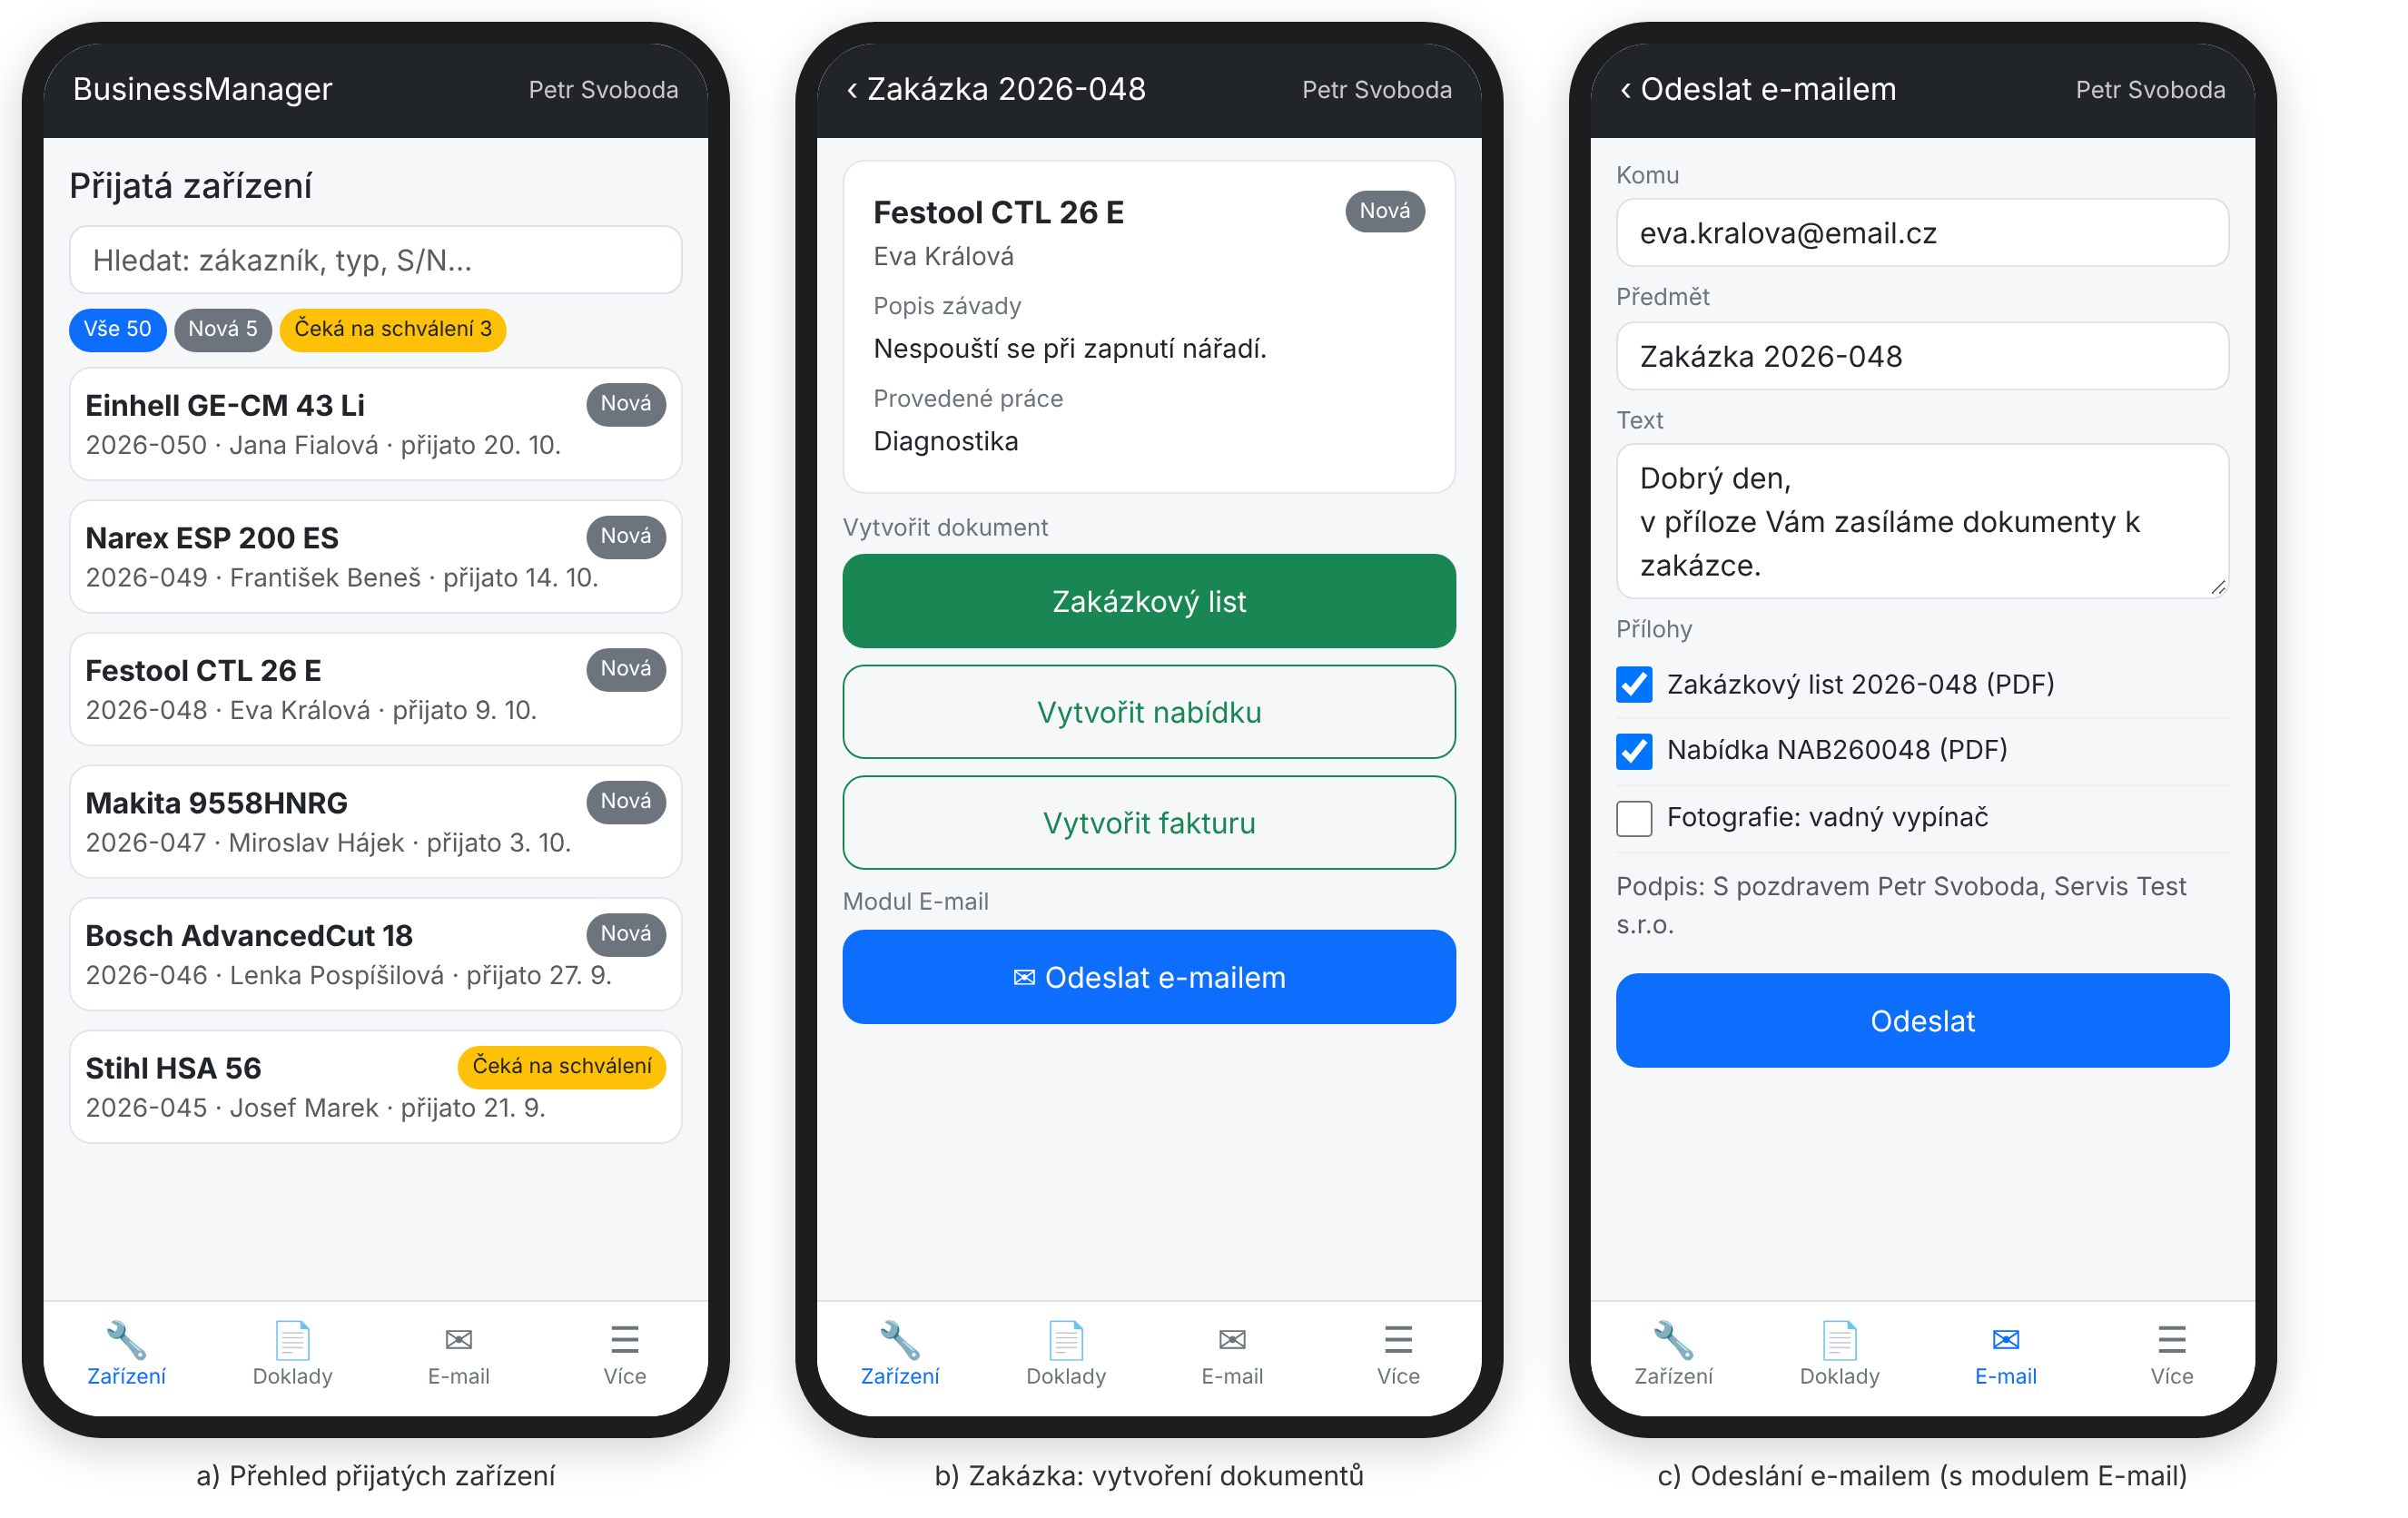
\includegraphics[width=\linewidth]{obrazky/rozvoj/mobilni-navrh.png}
\caption{Návrh zobrazení aplikace na telefonu v~plánovaném modulu Mobilní přístup: a)~přehled přijatých zařízení, b)~vytvoření dokumentů ze zakázky, c)~odeslání e-mailem (zdroj: vlastní návrh, data z~testovací databáze)}\label{obr:mobilni-navrh}
\end{figure}

Mimo moduly zůstávají možností rozvoje úpravy rozhraní podle doporučení z~oddílu~\ref{sec:ui-upravy} a~pohodlnější předávání faktur do účetnictví, pro které aplikace už vytváří elektronickou fakturu ve formátu ISDOC.

\chapter{Závěr}

Závěr je klíčovou kapitolou, která může nejvíce ovlivnit vaši obhajobu. Základní částí závěru je přehledné shrnutí výstupů práce tj. co jste udělali pro dosažení cílů práce. Je nutné se vyhnout hodnocení, zda tím byly splněny cíle práce, či nikoliv (to je úkol posudků a především komise).


\sloppy
\printbibliography[title=Seznam použitých zdrojů]

\appendix

\chapter{Externí přílohy}\label{sec:ep}

Zdrojový kód aplikace BusinessManager a~její dokumentace jsou zveřejněny pod licencí MIT v~repozitáři na GitHubu:\\ \url{https://github.com/MajkyyQ/BusinessManager}.

Dokumentace ve složce \path{docs/} popisuje aplikaci podrobněji, než umožňuje rozsah práce, a~text práce na ni na příslušných místech odkazuje. Na GitHubu se zobrazuje jako formátovaný text včetně diagramů. Strukturu repozitáře shrnuje tabulka~\ref{tab:repozitar}.

\begin{longtable}{p{0.36\textwidth}p{0.56\textwidth}}
\caption{Struktura repozitáře aplikace}\label{tab:repozitar}\\
\hline
\textbf{Soubor nebo složka} & \textbf{Obsah} \\
\hline
\endfirsthead
\hline
\textbf{Soubor nebo složka} & \textbf{Obsah} \\
\hline
\endhead
\path{README.md} & přehled aplikace a rychlá instalace ve Windows \\
\path{INSTALACE.md} & podrobný návod k instalaci, zálohování, obnově a řešení potíží \\
\path{docs/README.md} & rozcestník dokumentace \\
\path{docs/01-popis-aplikace.md} & účel aplikace a typický průběh práce \\
\path{docs/02-funkce.md} & popis všech funkcí z pohledu uživatele i systému \\
\path{docs/03-technologie.md} & použité technologie a důvody jejich volby \\
\path{docs/04-architektura.md} & architektura, zabezpečení, spuštění a nasazení \\
\path{docs/05-struktura-projektu.md} & struktura zdrojového kódu \\
\path{docs/06-tok-dat.md} & tok dat od zadání zakázky po dokument \\
\path{docs/07-databaze.md} & databázový model, diagramy a popis všech tabulek \\
\path{docs/databaze-tabulky.md} & referenční přehled sloupců generovaný z modelů \\
\path{docs/08-sablony-dokumentu.md} & systém šablon, editor šablon, export a import ISDOC \\
\path{docs/09-vyvoj-a-testovani.md} & spuštění pro vývoj a automatické testy \\
\path{docs/10-prvni-nastaveni.md} & co nastavit po instalaci: firma, role, zaměstnanci, typy úkonů \\
\path{config/}, \path{core/} & zdrojový kód aplikace Django \\
\path{Dockerfile}, \path{docker-compose.yml} & zabalení aplikace do kontejnerů \\
\path{instalace.bat}, \path{aktualizace.bat}, \path{zaloha.bat} & instalace, aktualizace a záloha ve Windows dvojklikem \\
\path{LICENSE} & licence MIT \\
\hline
\end{longtable}



\end{document}
